%!TEX program = xelatex

% safe參數解決與\!在內的多個衝突
% \sups命令可能被重定義,xeCJK放在tipa後
\RequirePackage[safe]{tipa}

\documentclass[a4paper, zihao=-4, linespread=1]{ctexrep}
\renewcommand{\CTEXthechapter}{\thechapter}
% 最小行間間距設定
\setlength{\lineskiplimit}{3pt}
\setlength{\lineskip}{3pt}

% 中文支持
\setCJKmainfont[BoldFont=Source Han Serif SC Bold]{Source Han Serif SC}
  \xeCJKsetup{CJKmath=true}
  \setCJKmathfont{KaiTi}  % 數學環境中使用楷體
\newCJKfontfamily[zhxinwei]\xinwei{STXinwei} % 定義新字體

% 顏色
\usepackage[table]{xcolor}
  \newcommand{\scol}[1]{\colorbox{#1}{\rule{0em}{1ex}}\,#1}
  
% 首字下沉
\usepackage{lettrine}

% 分欄
\usepackage{multicol}
  \setlength{\columnsep}{20pt}
  \setlength{\columnseprule}{0.4pt}

% 數學環境
\usepackage{mathdots} % 數學省略號,會重定義 dddot 和 ddddot
\usepackage{amsmath}  
  \newcommand{\ue}{\mathrm{e}}
  \newcommand{\ud}{\mathop{}\negthinspace\mathrm{d}} % 微分號
\usepackage{amssymb}
\usepackage{mathrsfs} % 線性代數字體
% overline的替代命令
\newcommand{\closure}[2][3]{{}\mkern#1mu\overline{\mkern-#1mu#2}}
\usepackage{yhmath} % \wideparen命令:弧AB
\usepackage{mathtools} % dcases環境,prescript命令
\usepackage{amsthm} % 定理環境
  \theoremstyle{definition}\newtheorem{laws}{Law}[section]
  \theoremstyle{plain}\newtheorem{ju}[laws]{Jury}
  \theoremstyle{remark}\newtheorem*{marg}{Margaret}
\usepackage{esint} % 多重積分,需放在amsmath後
% 箭頭與長等號
\usepackage{extarrows}
% 中括號的類二項式命令
\newcommand{\Bfrac}[2]{\genfrac{[}{]}{0pt}{}{#1}{#2}}

% 下劃線宏包
\usepackage[normalem]{ulem}
% LaTeX符號宏包
\usepackage{hologo}
	\newcommand{\xelatex}{\Hologo{XeLaTeX}}
  \newcommand{\bibtex}{\Hologo{BibTeX}}
  \newcommand{\biber}{\Hologo{biber}}
	\newcommand{\tikzz}{Ti\textit{k}Z}
	\newcommand{\bz}{B\'ezier}
% 其他符號
\usepackage{wasysym}
% 帶箱小頁
\usepackage{boxedminipage}
% 繪圖
\usepackage{tikz}
  \usetikzlibrary{calc,intersections,positioning,angles,quotes,decorations.pathmorphing,fit,backgrounds,through,svg.path,topaths,patterns}
  \newcommand{\tikzline}[1]{{#1\tikz{\draw[#1,line width=9](0,0)--(0.5,0);}}, }
% 最後一頁
\usepackage{lastpage}

% 奇怪的小定義
\newcommand{\dpar}{\\ \mbox{}}  % 空兩行
\newcommand{\qd}[1]{{\bfseries{#1}}}  % 強調
\newcommand{\co}[1]{{\bfseries{#1}}}  % Style of concept
\newcommand{\RED}[1]{{\color{cyan}{#1}}}
\newcommand{\cmmd}[1]{\fbox{\texttt{\char92{}#1}}}
\newcommand{\charef}[1]{第\ref{#1}章}
\newcommand{\secref}[1]{第\ \ref{#1}\ 節}
\newcommand{\pref}[1]{第\pageref{#1}頁}
\newcommand{\fref}[1]{圖\ref{#1}}
\newcommand{\tref}[1]{表\ref{#1}}

% Quote 環境
\newenvironment{QuoteEnv}[2][]
    {\newcommand\Qauthor{#1}\newcommand\Qref{#2}}
    {\medskip\begin{flushright}\small ——~\Qauthor\\
    \emph{\Qref}\end{flushright}}
% 字體調用
\newcommand{\myfont}[2]{{\fontfamily{#1}\selectfont #2}}

% 編號列表宏包,並自定義了三個列表
\usepackage[inline]{enumitem}
	\setlist[enumerate]{font=\bfseries,itemsep=0pt}
	\setlist[itemize]{font=\bfseries,leftmargin=\parindent}
	\setlist[description]{font=\bfseries\uline,labelindent=\parindent,itemsep=0pt,parsep=0pt,topsep=0pt,partopsep=0pt}

\newenvironment{fead}{	
    \begin{description}[font=\bfseries\uline,labelindent=\parindent,itemsep=0pt,parsep=0pt,topsep=0pt,partopsep=0pt]}
	{\end{description}}
% 帶寬度的
\newenvironment{para}{
	\begin{description}[font=\bfseries\ttfamily,itemsep=0pt,parsep=0pt,topsep=0pt,partopsep=0pt]}
	{\end{description}}
\newenvironment{feae}{
	\begin{enumerate}[font=\bfseries,labelindent=0pt,itemsep=0pt,parsep=0pt,topsep=0pt,partopsep=0pt]}
	{\end{enumerate}}
\newenvironment{feai}{
	\begin{itemize}[font=\bfseries,itemsep=0pt,parsep=0pt,topsep=0pt,partopsep=0pt]}
	{\end{itemize}}
\newenvironment{inlinee}
{\begin{enumerate*}[label=(\arabic*), font=\rmfamily, before=\unskip{:},itemjoin={{;}},itemjoin*={{,以及:}}]}
	{\end{enumerate*}。}

% 目錄和章節樣式
\usepackage{titlesec}
\usepackage{titletoc}   % 用於目錄

\titlecontents{chapter}[1.5em]{}{\contentslabel{1.5em}}{\hspace*{-2em}}{\hfill\contentspage}
\titlecontents{section}[3.3em]{}{\contentslabel{1.8em}}
	{\hspace*{-2.3em}}{\titlerule*[8pt]{$\cdot$}\contentspage}
\titlecontents*{subsection}[2.5em]{\small}{\thecontentslabel{} }{}{, \thecontentspage}[;\qquad][.]
% 章節樣式
\setcounter{secnumdepth}{3} % 一直到subsubsection
\newcommand{\chaformat}[1]{%
	\parbox[b]{.5\textwidth}{\hfill\bfseries #1}%
	\quad\rule[-12pt]{2pt}{70pt}\quad
	{\fontsize{60}{60}\selectfont\thechapter}}
\titleformat{\chapter}[block]{\hfill\LARGE\sffamily}{}{0pt}{\chaformat}[\vspace{2.5pc}\normalsize
	\startcontents\setlength{\lineskiplimit}{0pt}\printcontents{}{1}{\setcounter{tocdepth}{2}\songti}]
\titleformat*{\section}{\centering\Large\bfseries}
\titleformat{\subsubsection}[hang]{\bfseries\large}{\rule{1.5ex}{1.5ex}}{0.5em}{}
% 擴展章節
\newcommand{\starsec}{\noindent\fbox{\S\textit{注意:本章節是一個擴展閲讀章節。}}
	\\ \mbox{}}

\renewcommand{\contentsname}{目錄}
	\renewcommand{\tablename}{表}
	\renewcommand\arraystretch{1.2}	% 表格行距
	\renewcommand{\figurename}{圖}
% 設置不需要浮動體的表格和圖像標題
\setlength{\abovecaptionskip}{5pt}
\setlength{\belowcaptionskip}{3pt}
\makeatletter
\newcommand\figcaption{\def\@captype{figure}\caption}
\newcommand\tabcaption{\def\@captype{table}\caption}
\makeatother
% 圖表
\usepackage{array,multirow,makecell}
  \setlength\extrarowheight{2pt} % 行高增加
\usepackage{diagbox}
\usepackage{longtable}
\usepackage{graphicx,wrapfig}
  \graphicspath{{./tikz/}}
\usepackage{animate}
\usepackage{caption,subcaption}
  \captionsetup[sub]{labelformat=simple}
  \renewcommand{\thesubtable}{(\alph{subtable})}
% 三線表
\usepackage{booktabs}  

% 頁面修正宏包
\usepackage{geometry}
  \geometry{vmargin = 1in}

% 代碼環境
\usepackage{listings}
% 複製代碼時不復制行號
\usepackage{accsupp}
  \newcommand{\emptyaccsupp}[1]{\BeginAccSupp{ActualText={}}#1\EndAccSupp{}}
\usepackage{tcolorbox}
  \tcbuselibrary{listings,skins,breakable,xparse}

% global style
\lstset{
  basicstyle=\small\ttfamily,
  % Word styles
  keywordstyle=\color{blue},
  commentstyle=\color{green!50!black},
  columns=fullflexible,  % Avoid too sparse word spaces
  keepspaces=true,
  % Numbering
  numbers=left,
  numberstyle=\tiny\color{red!75!black}\emptyaccsupp,
  % Lines and Skips
  aboveskip=0pt plus 6pt,
  belowskip=0pt plus 6pt,
  breaklines=true,
  breakatwhitespace=true,
  emptylines=1,  % Avoid >1 consecutive empty lines
  escapeinside=``
}

% TikZ Language Hint
\lstdefinelanguage{tikzlang}{
  sensitive=true,
  morecomment=[n]{[}{]}, % nested comment
  morekeywords={
    draw,clip,filldraw,path,node,coordinate,foreach,pic,
    tikzset
  }
}

% 對於 tcolorbox 中 listings 庫的 ''tcblatex'' style 的重現,
% 添加了新的關鍵詞
\lstdefinestyle{latexcn}{
  language=[LaTeX]TeX,
  % More Keywords
  classoffset=0,
  texcsstyle=*\color{blue},
  moretexcs={
    % LaTeX extension
    chapter,section,subsection,setlength,
    thechapter,thesection,thesubsection,theequation,
    chaptermark,chaptername,appendix,
    bibname,refname,bibpreamble,bibfont,citenumfont,bibnumfmt,bibsep,
  },
  classoffset=1,
  texcsstyle=*\color{orange!75!black},
  moretexcs={
    % XeCJK & CTeX
    xeCJKsetup,setCJKmainfont,newCJKfontfamily,CJKfontspec,
    CTEXthechapter,songti,heiti,fangsong,kaishu,yahei,lishu,youyuan,
    % AMSmath / AMSsymb / AMSthm
    middle,text,tag,boldsymbol,mathbb,dddot,ddddot,iint,varoiint,
    dfrac,tfrac,cfrac,leftroot,uproot,underbracket,xleftarrow,xrightarrow,
    overset,underset,sideset,mathring,leqslant,geqslant,because,therefore,
    shortintertext,binom,dbinom,implies,thesubequation,
    impliedby,genfrac,theoremstyle,qedhere,
    % Other math packages
    wideparen,intertext,
    xlongequal,xLeftrightarrow,xleftrightarrow,xLongleftarrow,xLongrightarrow,
    % xcolor
    definecolor,color,textcolor,colorbox,fcolorbox,
    % hyperref
    hyperref,autoref,href,url,nolinkurl,
    % Graph & Table
    includegraphics,graphicspath,scalebox,rotatebox,animategraphics,
    newcolumntype,arraybackslash,multirow,captionsetup,
    thead,multirowcell,makecell,Xhline,Xcline,diagbox,
    toprule,midrule,bottomrule,DeclareFloatingEnvironment,
    % ulem
    uline,uuline,dashuline,dotuline,uwave,sout,xout,
    % fancyhdr
    lhead,chead,rhead,lfoot,cfoot,rfoot,
    fancyhf,fancyhead,fancyfoot,fancypagestyle,
    % fontspec
    newfontfamily,
    % titlesec & titletoc
    titlelabel,titleformat,titlespacing,titleline,titlerule,dottecontents,titlecontents,
    % enumitem
    setlist,
    % Listings & tcolorbox
    lstdefinelanguage,lstdefinestyle,lstset,lstnewenvironment,
    tcbuselibrary,newtcblisting,newtcbox,DeclareTCBListing
    % citation & index: natbib, imakeidx
    setcitestyle,printindex,
    % Other packages
    hologo,lettrine,endfirsthead,endhead,endlastfoot,columncolor,rowcolors,modulolinenumbers,MakeShortVerb,tikz,Hologo
  }
}

% cmd & envi
\newtcbox{\latexline}[1][green]{on line,before upper=\ttfamily\char`\\,
  arc=0pt,outer arc=0pt,colback=#1!10!white,colframe=#1!50!black,
  boxsep=0pt,left=1pt,right=1pt,top=1pt,bottom=1pt,
  boxrule=0pt,bottomrule=1pt,toprule=1pt}
\newtcbox{\envi}[1][violet!70!cyan]{on line,before upper=\ttfamily,
  arc=0pt,outer arc=0pt,colback=#1!10!white,colframe=#1!50!black,
  boxsep=0pt,left=1pt,right=1pt,top=1pt,bottom=1pt,
  boxrule=0pt,bottomrule=1pt,toprule=1pt}
% pkg
\newtcbox{\pkg}[1][orange!70!red]{on line,before upper={\rule[-0.2ex]{0pt}{1ex}\ttfamily},
  arc=0.8ex,colback=#1!30!white,colframe=#1!50!black,
  boxsep=0pt,left=1.5pt,right=1.5pt,top=1pt,bottom=1pt,
  boxrule=1pt}
\newcommand{\tikzkw}[1]{\texttt{#1}}

% tcblisting definitions
\newtcblisting{latex}{breakable,skin=bicolor,colback=gray!30!white,
  colbacklower=white,colframe=cyan!75!black,listing only, 
  left=6mm,top=2pt,bottom=2pt,fontupper=\small,
  listing options={style=latexcn}
}

\NewTCBListing{codeshow}{ !O{listing side text} }{
  skin=bicolor,colback=gray!30!white,
  colbacklower=pink!50!yellow,colframe=cyan!75!black,
  valign lower=center,
  left=6mm,righthand width=0.4\linewidth,fontupper=\small,
  % listing style
  listing options={style=latexcn},#1,
}

% Fix solution from the tcolorbox package author
\makeatletter
\tcbset{
  tikz upper/.style={before upper=\centering\tcb@shield@externalize\begin{tikzpicture}[{#1}],after upper=\end{tikzpicture}},%
  tikz lower/.style={before lower=\centering\tcb@shield@externalize\begin{tikzpicture}[{#1}],after lower=\end{tikzpicture}},%
}
\makeatother

% xparse library required
\NewTCBListing{tikzshow}{ O{} }{
  tikz lower={#1},
  halign lower=center,valign lower=center,
  skin=bicolor,colback=gray!30!white,
  colbacklower=white,colframe=cyan!75!black, 
  left=6mm,righthand width=3.5cm,listing outside text,
  listing options={language=tikzlang}
}

\NewTCBListing{tikzshowenvi}{ O{} }{
  halign lower=center,valign lower=center,
  skin=bicolor,colback=gray!30!white,
  colbacklower=white,colframe=cyan!75!black, 
  left=6mm,righthand width=3.5cm,listing outside text,
  listing options={language=tikzlang},#1
}
% inline tikz draw
%\newcommand{\tikzline}{def}

% 附錄
% \usepackage{appendix}
\renewcommand{\appendixname}{App.}

% 行號
\usepackage{lineno}

% 索引與參考文獻
\usepackage{imakeidx}
  \newcommand{\tikzidx}[1]{\index{\char`\\ #1}}
  \newcommand{\tikzoptstyle}[1]{\texttt{#1}}
  \newcommand{\tikzopt}[2][draw]{\tikzoptstyle{#2}\index{\char`\\ #1!#2}\ }
  \renewcommand{\indexname}{\tikzz 命令索引}
\makeindex[intoc]

\bibliographystyle{plain}
\renewcommand{\bibname}{參考文獻}
\usepackage[numindex,numbib]{tocbibind}
\usepackage[square,super,sort&compress]{natbib}

% 引用
\usepackage{hyperref}
\hypersetup{colorlinks, bookmarksopen = true, bookmarksnumbered = true, pdftitle=LaTeX-cn, pdfauthor=K.L Wu, pdfstartview=FitH}

\title{簡單粗暴\LaTeX\ }
\author{K.L Wu\\
  {\kaishu 本手冊是\href{https://github.com/wklchris/Note-by-LaTeX}{wklchris-GitHub}的\LaTeX{}-cn項目}
}
\date{當前版本號:v1.6.4-pre\\
  最後更新於:\today}

\begin{document}

\maketitle

\setlength{\lineskiplimit}{0pt}
\tableofcontents
\setlength{\lineskiplimit}{3pt}

\chapter{序}

\noindent{\Huge\xinwei 第一稿序}\dpar\dpar

其實在之前我是有一稿手冊的,開始撰寫的日期大概在2015年4月.但是自己覺得寫得太爛,因此索性推倒重寫了這一版.這一版的主要特徵是:
\begin{feae}
  \item 我希望能夠吸引初學者快速上手,解決手頭的問題.因此去掉了枯燥的講解和無窮無盡的宏包用法介紹,直接使用實例;
  \item 力求突出實用性.當然,也會提點一些可以深入學習的內容,讀者可以自行查閲,或者閲讀本手冊中的擴展閲讀章節(即帶星號*的章節).
  \item 本手冊使用的編輯器為\TeX\ Studio,而非之前的商業軟件WinEdt. 這使得學習\LaTeX\ 的門檻更低.當然了,你有權使用任何編輯器.
\end{feae}

手冊主體分為六大部分\cite{LHY2013latex,lamport1994latex,frank2004latex,partl2016,Casteleyn2016tikz,tikzmanual}:
\begin{fead}
\item[寫給讀者*] 介紹\LaTeX\ 背景、優缺點、適用情形.
\item[基礎] 包括標點、縮進、距離、章節、字體、顏色、註釋、引用、封面、目錄、列表、圖表、頁面等詳細內容.
\item[數學排版] 包括數學符號、公式、編號等內容.
\item[進階] 主要是自定義命令,幫助你更高效、更簡潔地書寫你的文檔.
\item[\tikzz\  繪圖*] 附加章節,需要讀者取消註釋後重編譯.
\item[附錄] 幫助你快速查找一些你想要的東西.
\end{fead}

由於工作全部由我一人完成,限於視野,難免存在錯漏之處.懇請讀者指正.如遇到的手冊中無法解決的問題,歡迎向我提出.推薦書目可參考本手冊附錄.

最後,還要感謝在\LaTeX\ 學習中為我解答疑惑的同學,特別是來自\LaTeX\ 度吧的吧友;本手冊中許多的解決方案都是由他們提供的.我謹在此記錄.

\vfill

\begin{flushright}
Mail: wklchris@hotmail.com\dpar

Chris Wu

September 17, 2016 於Davis, CA
\end{flushright}
\clearpage
\noindent{\Huge\xinwei 更新日誌:}\dpar\dpar

版本號以 $x.y.z$ 的形式公示.當$z=0$時,為決定正式 release 的版本.

v1.6.0 更新 --- 2017年6月15日:

v1.6.1 更新 --- 2017年8月9日;

v1.6.2 更新 --- 2017年10月5-15日.

v1.6.3 更新 --- 2018年3月22日.\dpar

以下內容中,未以括號註明的項是在v1.6.0中更新的.

\begin{feai}
\item 重要更新:
  \begin{feai}
  \item \textbf{\sout{\tikzz\  相關的內容停止更新}.原因是現有的其他軟件繪圖功能強大,導出為 pdf 格式的矢量圖後也易於調用;\tikzz\  相比之下學習成本過高.}\textcolor{red}{\textbf{筆者又決定重啓\tikzz\ 章節}}.(v1.6.3)
  \item \textbf{重新添加了 \tikzz\  章節} —— 不過仍是之前棄筆時的版本,預計將於 v1.7 更新.
  \item \textbf{增加了加快\xelatex 調用字體速度的方式}.參考“中文支持與CJK字體”一節\texttt{fc-cache}相關內容.(v1.6.1)
  \end{feai}
\item 字體更換:思源宋體.
\item 編輯了 Head.tex 文件,使之更易閲讀.
\item [添加]宏包\pkg{animate}:在 PDF 中展示動態圖.(v1.6.1)
\item [添加]宏包\pkg{tocbibind}:
  \begin{feai}
  \item 將目錄本身編入目錄項.
  \item 將參考文獻章節編號、編入目錄項.
  \item 將索引章節編號、編入目錄項.
  \end{feai}
\item [更新]宏包\pkg{dcolumn},更詳細説明了如何在表格中使用小數點對齊.(v1.6.2)
\item [更新]宏包\pkg{fancyvbr}:更詳細説明了抄錄環境\envi{BVerbatim},如何提供居中支持.(v1.6.2)
\item [更新]宏包\pkg{xeCJK}:
  \begin{feai}
  \item 參數 CJKspace.該功能在新版宏包中已修復.
  \item 命令 \latexline{setCJKmainfont},可指定字體文件名.
  \end{feai}
\item 數學內容:
  \begin{feai}
  \item [添加]宏包\pkg{extarrows}:長等號命令.
  \item [添加]命令\latexline{numberthis},用於給多行公式中的某行編號.(v1.6.2)
  \item [添加]命令\latexline{allowdisplaybreaks},用於支持多行公式環境換頁.
  \end{feai}
\item 拆分了文檔,並修改了“文檔拆分”一節的內容.(v1.6.3)
\item 修復了一些錯別字與無效的文檔內跳轉鏈接.
\end{feai}

\mbox{}

更早版本的更新細節,請到\href{https://github.com/wklchris/Note-by-LaTeX/releases}{Project Release Webpage}瀏覽.

% Main Contents

%!TEX root = ../LaTeX-cn.tex
\chapter{\mbox{寫給讀者}*}

我見過許多朋友初試\LaTeX\ ,他們都感到非常不能理解。主要有以下幾個疑問:
\begin{feae}
\item “我平常使用MS Word,似乎也能完成科技排版工作,那麼為什麼我還需要\LaTeX\ ?”\hfill \textit{——見“為什麼需要\LaTeX\ ?”一節。}
\item “\LaTeX\ 看上去不像是排版工具,更像是編程語言。我討厭用寫代碼一樣的方式來寫文章。”\hfill \textit{——文本文件使你更專注於內容而不是排版細節。}
\item “\LaTeX\ 能生成doc文件嗎?我平時上交作業/提交匯報時難道使用不便修改pdf文件麼?”\hfill \textit{——見“\LaTeX\ 生成的文件格式?”一節。}
\end{feae}

本章希望能解決讀者的這些疑問,讓讀者對於\LaTeX\ 有基礎的瞭解,再決定是否需要學習。當然,如果你是被迫進入了\LaTeX\ 這個坑,你也可以閲讀本章,或許本章能讓你喜歡上\LaTeX\ 呢。

\section{什麼是\LaTeX\ ?}
先講\TeX\ (讀音類似於“泰赫”)。

\TeX\ 是Knuth\footnote{Donald Ervin Knuth(高德納,1938--),現代計算機科學的先驅者,斯坦福大學計算機系的終身榮譽教授,圖靈獎和馮諾依曼獎得主,\TeX\ 和 \hologo{METAFONT} 的發明人。同時也是業內經久不衰的著作\emph{The Art of Computer Programming}的作者。}研發的免費、開源的排版系統,其初衷是為了“改變排版界糟糕的排版技術”,並用於排版他的著作《計算機程序設計藝術》。

\TeX\ 對於讀者來説應該是底層的內容,如果你有興趣,可以閲讀Knuth著的\emph{The \TeX\ book},這本書是學習\TeX\ 最權威的材料,沒有之一。在本手冊的參考文獻中也給出了其他\TeX\ 學習的資料。\dpar

再講\LaTeX\ (讀音類似於“拉泰赫”)。

\LaTeX\ 是基於\TeX\ 的宏\footnote{“宏(Macro)”是一個計算機概念,指用單個命令或操作完成一系列底層命令或操作的組合。}集,其作者是Dr.~Lamport\footnote{Leslie Lamport(1941--),美國計算機科學家,圖靈獎和馮諾依曼獎得主。};其姓氏開頭兩個字母La與底層排版系統\TeX\ 相結合,就組成了名稱\LaTeX\ 。\LaTeX\ 在\TeX\ 基礎上定義了眾多的宏命令,使得用户可以更方便地進行排版。本手冊的參考文獻中就有他的作品。

\LaTeX\ 現在的版本是\LaTeXe ,意思是2.x版而沒到3.0版。錯位排版的字母E和字母A暗示了它是排版系統。在無法這樣輸出的場合,請寫作LaTeX和LaTeX~2e。

\section{\TeX\ 與\LaTeX\ 的優缺點}
\TeX\ 的優點:\qd{穩定、精確、美觀}。底層的\TeX\ 系統已經很多年沒有進行大的變動了,因為它注重\uline{穩定};\TeX\ 系統可以讓你把排版內容通過數字參數的方式寫到任意的位置,量化的參數意味着\uline{精確};\TeX\ 底層的空距調整機制,以及對於數學公式近乎完美的支持,則確保了排版效果的\uline{美觀}。

\LaTeX\ 是基於\TeX\ 的,自然不會拋棄上述\TeX\ 的優點。具體包括:
\begin{feai}
\item 排版出來就是印刷品。專業而美觀。
\item 易用、全面的數學排版支持,無出其右。
\item 撰寫文檔時不會被文檔排版細節干擾精力。你可以使用之前自定義的模板,或者方便地在文字組織完畢後調整你的模板,以輕鬆達到滿意的效果。
\item 複雜的排版功能支持,比如圖表目錄、索引、參考文獻管理、高度自定義的目錄樣式、雙欄甚至多欄排版。
\item 豐富的功能以及易尋的幫助文檔。眾多的\LaTeX\ 宏包賦予了\LaTeX\ 強大的擴展功能,它們都自帶文檔供你學習。
\item 源文件是\RED{文本文件}\footnote{文本文件的另一個優點是易於進行版本控制,比如利用git. 你可以方便地比較你相比上次修改了什麼內容,也可以方便地恢復到之前某個時刻的版本。}。你可以在任何設備、任何文本編輯器中書寫文檔內容,無須擔心複製時格式的變化;最後粘貼到同一個tex文件中編譯即可。
\item 跨平台,免費,開源。
\end{feai}

那缺點呢?我認為主要有:
\begin{feai}
\item 入門門檻高。想要熟練地使用\LaTeX\ 並輕鬆地編寫有自己的風格的文檔,不是一兩天就能夠達到的。
\item 並非“所見即所得”,需要編譯才能看到效果。編譯查錯有時令人惱火。
\item 完善一個自己的模板可能需要很長的時間。儘管\LaTeX\ 原生定義的模板能夠滿足絕大多數場合的需要。
\item 排版長表格有些複雜。但作為補充,在表格內插入數學公式是非常簡單的。
\end{feai}

\section{為什麼需要\LaTeX\ ?}
你可能基於以下原因學習\LaTeX\ :
\begin{feae}
\item 你的投稿對象要求你使用\LaTeX\ 排版,而不是MS Word——這種情況對沒聽説過\LaTeX\ 的你來説,真是糟糕透了。
\item 你需要在多個設備上撰寫同一份文檔。但你發現把內容在多個文檔間複製粘貼時,格式總是會出現問題。
\item 你受夠了MS Word自帶的公式編輯器,或者你覺得購買的插件MathType的效果也不盡如人意。但你經常需要排版公式。
\item 你想參加某個科學競賽,比如MCM,然後你發現你的朋友用的一個叫\LaTeX\ 的東西似乎還不錯。
\item 你想出版一本書,或者投稿你的作品——結果他們告知你如果你使用\LaTeX\ 而不是MS Word攥寫原稿件,他們會更快地把作品印刷出來。
\item 呃……也許,你只是喜歡學習新事物?
\end{feae}

對於科研工作者或者在校研究生,我認為\LaTeX\ 是非常優秀的工具。如果你是本科生,或者更年輕的羣體,你也可以先學習\LaTeX\ ,因為到了研究生和工作中,學習這類基礎工具的時間可能就非常有限了。

\section{MS Word難道不優秀嗎?}
我想説的是,\qd{MS Word當然是優秀的軟件}。但是它與\LaTeX\ 的定位不同,所以它們分別適用於不同場合。前者注重簡單組織內容,後者注重排版效果。

在\uline{排版書籍、科學文檔}方面,\LaTeX\ 非常專業、美觀,公式支持性極佳,幾乎所有參數你都可以量化調整。如果你想\uline{高度自定義一份文件},比如擁有特殊幾何、顏色元素,且易於更改模板的簡歷,\LaTeX\ 可以完全獨當一面。在這些這方面,MS Word是無法匹敵\LaTeX\ 的。

但是如果你只是為了生成\uline{非正式的文檔},比如1--2頁的作業稿;或者只是一份\uline{易於別人修改的非科學稿件},比如一份需要同事修改的演講稿……那你無須使用\LaTeX\ 。這些方面,\LaTeX\ 無疑是比不上MS Word的。

\section{\LaTeX\ 生成的文件格式?}
一般廣為使用的是pdf,以及dvi的格式。\LaTeX\ 無法生成doc或者docx擴展名文件,因為那是屬於MS的商用格式,兩者的工作機理也完全不同。

所以很遺憾,如果你身處一個要求你“必須提交docx”的環境中,那麼\LaTeX\ 對你並不是一個好選擇。但我想指出的是,這是穩定、優秀的pdf格式沒有得到你身處環境認可的遺憾——pdf也可以方便地添加批註,並在不同設備的顯示上有更好的穩定性。
%!TEX root = ../LaTeX-cn.tex
\chapter{\LaTeX{}基礎}
\section{第一份文稿}

編輯器的配置大概是需要講解一下的,畢竟對於初學者來説是很頭疼的事情。本手冊就以\TeX\ Studio為例進行配置。首先你應該安裝一個\TeX{} Live,它是完全免費的,網址:\url{http://tug.org/texlive/}.

雖然它體積較大,但是卻是最一勞永逸、最不需要花時間去配置的方法,同時它大概也是功能支持最強的\LaTeX\ 發行版。

打開\TeX\ Studio後,選擇選項$\rightarrow$ 設置\TeX\ Studio $\rightarrow$ 構建$\rightarrow$ 默認編譯器,選擇\xelatex{}. 這主要是基於中文文檔編譯的考慮,同時\xelatex 也能很好地編譯英文文檔。我建議始終使用它作為默認編譯器。\dpar

之後你可以在窗口輸入一篇小文檔,並保存為tex擴展名的文件進行測試:
\begin{latex}
\documentclass{ctexart}
\begin{document}
    Hello, world!
    你好,世界!
\end{document}
\end{latex}

點擊編譯按鈕生成,F7查看。生成的pdf在你的tex文件保存目錄中。具體各行的含義我們會在後文介紹。

\section{認識\LaTeX}
\subsection{命令與環境}
\LaTeX\ 中的\co{命令}通常是由一個反斜槓加上命令名稱,再加上花括號內的參數構成的(有的命令不帶參數,例如:\latexline{TeX})。
\begin{latex}
\documentclass{ctexart}
\end{latex}

如果有一些選項是備選的,那麼通常會在花括號前用方括號標出。比如:
\begin{latex}
\documentclass[a4paper]{ctexart}
\end{latex}

還有一種重要指令叫做\co{環境}。它被定義於控制命令\latexline{begin\{environment\}} 和\latexline{end\{environment\}}間的內容。比如:
\begin{latex}
\begin{document}
...內容...
\end{document}
\end{latex}

環境如果有備選參數,只需要寫在\latexline{begin[...]\{name\}}這裏就行。

注意:不帶花括號的命令後面如果想打印空格,請加上\RED{一對內部為空的花括號}再鍵入空格。否則空格會被忽略。例如:\verb+\LaTeX{} Studio+.

\subsection{保留字符}

\LaTeX\ 中有許多字符有着特殊的含義,在你生成文檔時不會直接打印。例如每個命令的第一個字符:反斜槓。單獨輸入一個反斜槓在你的行文中不會有任何幫助,甚至可能產生錯誤。\LaTeX\ 中的保留字符有:
\begin{center}
\texttt{\# \$ \% \^ \& \_ \{ \} \char92}
\end{center}

它們的作用分別是:
\begin{para}
\item[\#{}:] 自定義命令時,用於標明參數序號。
\item[\${}:] 數學環境命令符。
\item[\%{}:] 註釋符。在其後的該行命令都會視為註釋。如果在回車前輸入這個命令,可以防止行末\LaTeX\ 插入一些奇怪的空白符。
\item[\^{}:] 數學環境中的上標命令符。
\item[\&{}:] 表格環境中的跳列符。
\item[\_{}:] 數學環境中的下標命令符。
\item[\{與\}:] 花括號用於標記命令的必選參數,或者標記某一部分命令成為一個整體。
\item[\char92{}:] 反斜槓用於開始各種\LaTeX\ 命令。
\end{para}

以上除了反斜槓外,均能用前加反斜槓的形式輸出。即你只需要鍵入:
\begin{center}
\verb|\# \$ \% \^ \& \_ \{ \}|
\end{center}

唯獨反斜槓的輸出比較頭痛,你可以嘗試:
\begin{codeshow}
$\backslash$ \textbackslash
\texttt{\char92}
\end{codeshow}

其中命令\latexline{char[num]}是一個特殊的命令,使用環境需要是tt字體環境,用於輸出ASCII碼對應的字符;92對應的即反斜槓。你也可以用\latexline{char`}後加字符的方式輸出你想輸出的命令,但需要包裹在\latexline{texttt}或者\latexline{ttfamily}內。如果想輸出的字符是保留字符,需要再加一個反斜槓。
\begin{verbatim}
\texttt{\char`~} % 輸出一個波浪線
\texttt{\char`\\} % 輸出保留字反斜槓
\texttt{\char`@} % 實際上可直接輸入@
\end{verbatim}

另外需要説明的是,上例提及的波浪線{\texttt{\~}}用來輸出一個禁止在該處斷行的空格,也不能夠直接輸出。嘗試:
\begin{codeshow}
a $\sim$ b
a\~ b
a\~{} b
a\textasciitilde b
\end{codeshow}

\subsection{導言區}
任何一份\LaTeX{}文檔都應當包含以下結構:
\begin{latex}
\documentclass[`\itshape options`]{doc-class}
\begin{document}
    ...
\end{document}
\end{latex}

其中,在語句\latexline{begin\{document\}}之前的內容稱為\co{導言區}。導言區可以留空,以可以進行一些文檔的準備操作。你可以粗淺地理解為:\RED{導言區即模板定義}。\dpar

文檔類的參數doc-class和可選選項{\textit{options}}有\tref{tab:documentclass}取值:
\begin{table}[!htb]
    \centering
	\caption{文檔類和選項}
	\label{tab:documentclass}
	\begin{tabular}{p{5em} @{\ -\ } p{24em}}
		\hline
		\multicolumn{2}{l}{\bfseries doc-class文檔類\footnotemark} \\
		\hline
		article   & 科學期刊,演示文稿,短報告,邀請函。\\
		proc      & 基於article的會議論文集。\\
		report    & 多章節的長報告、博士論文、短篇書。\\
		book      & 書籍。\\
		slides    & 幻燈片,使用了大號Scans Serif字體。\\
		\hline
		\multicolumn{2}{l}{\bfseries\itshape options} \\
		\hline
		字體     & 默認10pt,可選11pt和12pt.\\
		頁面方向 & 默認豎向portrait,可選橫向landscape。\\
		紙張尺寸 & 默認letterpaper,可選用a4paper, b5paper等。\\
		分欄     & 默認onecolumn,還有twocolumn。\\
		雙面打印 & 有oneside/twoside兩個選項,用於排版奇偶頁。article/report默認單面。\\
		章節分頁 & 有openright/openany兩個選項,決定是在奇數頁開啓新頁或是任意頁開啓新頁。注意article是沒有chapter(``章'')命令的,默認任意頁。\\
		公式對齊 & 默認居中,可改為左對齊fleqn;默認編號居右,可改為左對齊leqno。\\
		草稿選項 & 默認final,可改為draft,使行溢出的部分顯示為黑塊。\\
		\hline
	\end{tabular}
\end{table}

在本文中,多數的文檔類提及的均為report/book類。如果有article類將會特別指明。其餘的文檔類不予説明。本手冊排版即使用了report類。\dpar

在導言區最常見的是\co{宏包}的加載工作,命令形如:\latexline{usepackage\{package\}}。通俗地講,宏包是指一系列已經制作好的功能``模塊'',在你需要使用一些原生\LaTeX\ 不帶有的功能時,只需要調用這些宏包就可以了。比如本文的代碼就是利用\pkg{listings}宏包實現的。

宏包的具體使用將參在各部分內容説明中進行講解。如果你想學習一個宏包的使用,按Win+R組合鍵呼出運行對話框,輸入texdoc加上宏包名稱即可打開宏包幫助pdf文檔。例如:\verb|texdoc xeCJK|。

\footnotetext{此外還有\pkg{beamer}宏包定義的beamer文檔類,常用於創建幻燈片。}

\subsection{錯誤的排查}
\label{subsec:debug}
在編輯器界面上,下方的日誌是顯示編譯過程的地方。在你編譯通過後,會出現這樣的字樣:
\begin{feai}
	\item {\qd{Errors錯誤}}:嚴重的錯誤。一般地,編譯若通過了,該項是零。
	\item {\qd{Warnings警告}}:一些不影響生成文檔的瑕疵。
	\item {\qd{Bad Boxes壞箱}\footnote{Box是\LaTeX{}中的一個特殊概念,具體將在\hyperref[sec:box]{這裏}進行講解。}}:指排版中出現的長度問題,比如長度超出(Overfull)等。後面的Badness表示錯誤的嚴重程度,程度越高數值越大。這類問題需要檢查,排除Badness高的選項。
\end{feai}

你可以向上翻閲日誌記錄(即.log文件),來找到Warning開頭的記錄,或者Overfull/ Underfull開頭的記錄。這些記錄會指出你的問題出在哪一行(比如line 1-2) 或者在pdf的哪一頁(比如active [12]。注意,這個12表示計數器計數頁碼,而不是文件打印出來的真實頁數)。此外你還需要了解:
\begin{feai}
	\item 值得指出的是,由於\LaTeX{}的編譯原理(第一次生成aux文件,第二次再引用它),目錄想要合理顯示\qd{需要連續編譯兩次}。在連續編譯兩次後,你會發現一些Warnings會在第二次編譯後消失。在\TeX\ Studio中,你可以只單擊一次“構建並查看”,它會檢測到文章的變化並自動決定是否需要編譯兩次。
	\item 對於大型文檔,尋找行號十分痛苦。你需要學會合理地拆分tex文件,參閲\secref{sec:include}的內容。
\end{feai}

這裏也推薦宏包\pkg{syntonly},在導言區加入它支持的\latexline{syntaxonly}命令,會只排查語法錯誤而不生成任何文檔,這可以使你更快地編譯。不過它似乎不太穩定,例如本文檔可以正常編譯,但是使用該命令時則會出錯。

\subsection{文件輸出}
\LaTeX{}的輸出一般推薦pdf格式,由\LaTeX\ 直接生成dvi的方法並不推薦。

你在tex文檔的文件夾下可能看到的其他文件類型:
\begin{tabbing}
	.sty{\hspace{2em}}\=宏包文件\\
	.cls	\> 文檔類文件。\\
	.aux    \> 用於儲存交叉引用信息的文件。因此,在更新交叉引用(公式編號、\\
	\> 大綱級別)後,需要編譯兩次才能正常顯示。\\
	.log    \> 日誌。記錄上次編譯的信息。\\
	.toc    \> 目錄文件。\\
	.lof    \> 圖形目錄。\\
	.lot    \> 表格目錄。\\
	.idx    \> 如果文檔中包含索引,該文件用於儲存索引信息。\\
	.ind	\> 索引記錄文件。\\
	.ilg	\> 索引日誌文件。\\
	.bib	\> \bibtex 參考文獻數據文件。\\
	.bbl	\> \bibtex 生成的參考文獻記錄。\\
	.bst	\> \bibtex 模板。\\
	.blg	\> \bibtex 日誌。\\
	.out	\> \texttt{hyperref}宏包生成的pdf書籤記錄。
\end{tabbing}

有時\LaTeX\ 的編譯出現異常,你需要刪除文件夾下除了tex以外的文件再編譯。此外,在某些獨佔程序打開了以上的文件時(比如用Acrobat打開了pdf),編譯可能出現錯誤。請在編譯時確保關閉這些獨佔程序。

\section{標點與強調}
英文符號$|<>+=$一般用於數學環境中,如果在文本中使用,請在它們兩側加上“\$”。如果你在\LaTeX\ 中直接輸入大於、小於號而不把它們放在數學環境中,它們並不會被正確地打印。你應該使用\latexline{textgreater}, \latexline{textless}命令。

在部分科技文章中,中文的句號可能使用全角圓點“.”\footnote{這個標點是 U+FF0E,稱為 FULLWIDTH FULL STOP。},而不是平常的“。”,也不是正常的英文句點“.”。這個符號很難正常輸入;你可以先輸入正常句點,最後再替換。

\subsection{引號}
英文單引號並不使用兩個\verb|'|符號組合。左單引號是重音符\verb|`|(鍵盤上數字1左側),而右單引號是常用的引號符。英文中,\RED{左雙引號就是連續兩個重音符}。

英文下的引號嵌套需要藉助\latexline{thinspace}命令分隔,比如:
\begin{codeshow}[listing side text, listing options={escapeinside=++}]
``\thinspace`Max' is here.''
\end{codeshow}
% 這裏臨時修改了listing的escapeinside, 使得這一行代碼也可以被 codeshow 環境表示, 也使得行文風格更加統一
中文下的單引號和雙引號你可以用中文輸入法直接輸入。

\subsection{破折、省略號與短橫}
英文的短橫分為三種:
\begin{feai}
\item 連字符:輸入一個短橫:\verb|-|,效果如daughter-in-law
\item 數字起止符:輸入兩個短橫:\verb|--|,效果如:page 1--2
\item 破折號:輸入三個短橫:\verb|---|,效果如:Listen---I'm serious.
\end{feai}

中文的破折號你也許可以直接使用日常的輸入方式。中文的省略號同樣。但是注意,英文的省略號使用\latexline{ldots}這個命令而不是三個句點。

\subsection{強調:粗與斜}
\LaTeX\ 中專門有個叫做\latexline{emph\{text\}}的命令,可以強調文本。對於通常的西文文本,上述命令的作用就是斜體。如果你對一段已經這樣轉換為斜體的文本再使用這個命令,它就會取消斜體,而成為正體。

西文中一般採用上述的斜體強調方式而不是粗體,例如在説明書名的時候可能就會使用以上命令。關於字體的更多內容參考\hyperref[sec:font]{字體}這一節。

\subsection{下劃線與刪除線}
\LaTeX\ 原生提供的\latexline{underline}命令簡直爛的可以,建議你使用\pkg{ulem}宏包下的\texttt{uline}命令代替,它還支持換行文本。\pkg{ulem}宏包還提供了一些實用命令:

\begin{codeshow}
\uline{下劃線} \\
\uuline{雙下劃線} \\
\dashuline{虛下劃線} \\
\dotuline{點下劃線} \\
\uwave{波浪線} \\
\sout{刪除線} \\
\xout{斜刪除線}
\end{codeshow}

需要注意的是,\pkg{ulem}宏包重定義了\latexline{emph}命令,\RED{使得原來的加斜強調變成了下劃線、原來的兩次強調就取消強調變成了兩次強調就雙下劃線}。通過宏包的normalem選項可以取消這個更改:\verb|\usepackage[normalem]{ulem}|。

\subsection{其他}
角度符號或者温度符號需要藉助數學模式\verb|$...$|輸入:

\begin{codeshow}
$30\,^{\circ}$三角形 \\
$37\,^{\circ}\mathrm{C}$
\end{codeshow}

歐元符可能需要用到\pkg{textcomp}宏包支持的\latexline{texteuro}命令。

其次是千位分隔位,比如\verb|1\,000\,000|。如果你不想它在中間斷行就在外側再加上一個\latexline{mbox}命令:\latexline{mbox\{1\char`\\,000\char`\\,000\}}。也可以使用\pkg{numprint}或者\pkg{siunitx}宏包中的相關命令。

再次是注音符號,比如\^o,也常用於拼音聲調,參考\hyperref[app:phonetic]{注音符號表}部分的附錄內容。如果你想輸入音標,請使用tipa宏包\footnote{tipa會重定義\latexline{!}命令,因此請使用\latexline{negthinspace}代替;或在\pkg{xeCJK}與\pkg{amsmath}宏包前加載,並使用safe選項。具體可以參見本手冊的 Head.tex 文件。},同樣參考附錄A。

最後,介紹\pkg{hologo}宏包,它可以輸出許多\TeX\ 家族標誌。其實\LaTeX\ 原生自帶了\latexline{LaTeX}, \latexline{TeX}等命令。而hologo宏包支持的命令有:

\begin{codeshow}
% 大寫H表示符號的首字母也大寫
\hologo{XeLaTeX} \Hologo{BibTeX}
\end{codeshow}

\section{格式控制}
首先了解一下\hologo{LaTeX}的長度單位:
\begin{fead}
  \item[pt] point,磅。\label{sec:length}
  \item[pc] pica。1pc=12pt,四號字大小
  \item[in] inch,英寸。1in=72.27pt
  \item[bp] bigpoint,大點。1bp=$\frac{1}{72}$in
  \item[cm] centimeter,釐米。1cm=$\frac{1}{2.54}$in
  \item[mm] millimeter,毫米。1mm=$\frac{1}{10}$cm
  \item[sp] scaled point。\Hologo{TeX} 的基本長度單位,1sp=$\frac{1}{65536}$pt
  \item[em] 當前字號下,大寫字母M的寬度。
  \item[ex] 當前字號下,小寫字母x的高度。
\end{fead}

然後是幾個常用的長度宏,更多的長度宏使用會在表格、分欄等章節提到。
\begin{latex}
\textwidth % 頁面上文字的總寬度,即頁寬減去兩側邊距。
\linewidth % 當前行允許的行寬。
\end{latex}

有時候你可以使用可變長度,比如“\texttt{5pt plus 3pt minus 2pt}”,表示一個能收縮到3pt也能伸長到8pt的長度。直接使用倍數也是允許的,例如:1.5\latexline{parindent}等。

我們通常使用\latexline{hspace}和\latexline{vspace}這兩個命令控制特殊的空格,具體的使用方法參考\hyperref[sec:hvspace]{水平和豎直距離}這一節。

\subsection{空格、換行與分段}
在\LaTeX\ 中,多個空格會被視為一個,多個換行也會被視為一個。如果你想要禁止\LaTeX\ 在某個空格處的換行,將空格用\texttt{\char126}命令替代即可,比如“\texttt{Fig.\char126 8}”。

通常的換行方法非常簡單:\hologo{LaTeX}會自動轉行,然後在每一段的末尾,只需要輸入兩個回車即可完成分段。如果需要一個空白段落(實質是一個空白行),先輸入兩個回車,再輸入\latexline{mbox\{\}},最後再輸入兩個回車即可。你可以用\latexline{par}來產生一個帶縮進的新段。

在下劃線一節的例子中已經給出了強制換行的方式,即兩個反斜:\latexline{\char`\\}. 不過這樣做的缺點在於下一行段首縮進會消失,這個命令也的確一般\RED{不用於}正文換行;\textbf{正文中想要換行,請直接使用兩個回車}。

段落之間的距離由\latexline{parskip}控制,默認\texttt{0pt plus 1pt}. 
\begin{latex}
\setlength{\parskip}{0pt}
\end{latex}

宏包\pkg{lettrine}能夠產生首字下沉的效果:
\begin{codeshow}
\lettrine{T}{his} is an example. Hope you like this package, and enjoy your \LaTeX\ trip!
\end{codeshow}

\subsection{分頁}
用\latexline{newpage}命令開始新的一頁。

用\latexline{clearpage}命令清空浮動體隊列\footnote{參見\hyperref[sec:float]{浮動體}這一節的內容。},並開始新的一頁。

用\latexline{cleardoublepage}命令清空浮動體隊列,並在偶數頁上開始新的一頁。

注意:以上命令都是基於\latexline{vfill}的。如果要連續新開兩頁,請在中間加上一個空的箱子(\latexline{mbox\{\}}),如\latexline{newpage\char`\\mbox\{\}\char`\\newpage}。

\subsection{縮進、對齊與行距}
英文的段首不需要縮進。但是對中文而言,段首縮進需要藉助\pkg{indentfirst}宏包來完成。你可能還需要使用\latexline{setlength{\char`\\parindent}\{2em\}}這樣的命令來設置縮進距離。如果在句首強制取消縮進,你可以在段首使用\latexline{noindent}命令。

\LaTeX\ 默認使用兩端對齊的排版方式。你也可以使用\envi{flushleft}, \envi{flushright}, \envi{center}這三種環境來構造居左、居中、居右三種效果。特殊的\latexline{centering}命令常常用在環境內部(或者一對花括號內部),以實現居中的效果。但請儘量用\envi{center}環境代替這個老舊的命令。類似的命令還有\latexline{raggedleft}來實現居右,\latexline{raggedright}來實現居左。更多的空格控制請參考\hyperref[sec:hvspace]{這一節}。

插入製表位、懸掛縮進、行距等複雜的調整參考\hyperref[sec:hvspace]{這部分}的內容。

\section{字體與顏色}
\label{sec:font}
這一節只討論行文中字體使用。數學環境內字體使用請參考\hyperref[sec:mathfont]{這一節}的內容。

\subsection{字族、字系與字形}
字體(typeface)的概念非常令人惱火,在電子化時代,基本上也都以字體(font)作為替代的稱呼。宋體、黑體、楷體,這屬於\co{字族};對應到西文就是羅馬體、等寬體等。加粗、加斜屬於\co{字系和字形}。五號、小四屬於\co{字號}。這三者大概可以並稱\co{字體}\footnote{本文中的字族、字系等稱呼難以找到統一標準,可能並不是準確的名稱。}。

\subsection{中西文“斜體”}
首先需要明確一點:\RED{漢字沒有加斜體}。平常我們看到的加斜漢字,通常是幾何變換得到的結果,非常的粗糙,並不嚴格滿足排版要求;而真正的字形是需要精細的設計的。同時,漢字字體裏面也很少有加粗體的設計。

西文一般設有加斜,但是這與“斜體”並不是同一回事。加斜是指某種字族的Italy字系;而斜體,是指Slant字族。在行文中表強調時使用的是前者;在Microsoft Word等軟件中看到的傾斜的字母\textit{I},也代表前者。

\subsection{原生字體命令}
\LaTeX\ 提供了基本的字體命令,包括\tref{tab:fontcommand}中顯示的內容。
\begin{table}[!ht]
\centering
\caption{\LaTeX\ 字體命令表}
\label{tab:fontcommand}
\begin{tabular}{p{3em}<{\centering} @{\ -\quad} l @{\quad-\quad} p{18em}}
\hline
字族 & \latexline{rmfamily} & 把字體置為{\rmfamily Roman}羅馬字族。\\
     & \latexline{sffamily} & 把字體置為{\sffamily Sans Serif}無襯線字族。\\
     & \latexline{ttfamily} & 把字體置為{\ttfamily Typewriter}等寬字族。\\
\hline
字系 & \latexline{bfseries} & 粗體{\bfseries BoldSeries}字系屬性。\\
     & \latexline{mdseries} & 中粗體{\mdseries MiddleSeries}字系屬性。\\
\hline
字形 & \latexline{upshape}  & 豎直{\upshape Upright}字形。 \\
     & \latexline{slshape}  & 斜體{\slshape Slant}字形。 \\
     & \latexline{itshape}  & 強調體{\itshape Italic}字形。 \\
     & \latexline{scshape}  & 小號大寫體{\scshape Scap}字形。 \\
\hline
\multicolumn{3}{l}{\ttfamily 如果臨時改變字體,使用\latexline{textrm}, \latexline{textbf}這類命令。}\\
\hline
\end{tabular}
\end{table}

字族、字系、字形三種命令是互相獨立的,可以任意組合使用。但這種複合字體的效果有時候無法達到(因為沒有對應的設計),比如\latexline{scshape}字形和\latexline{bfseries}字系。\LaTeX\ 會針對這種情況給出警告,但仍可以編譯,只是效果會不同於預期。

如果在文中多次使用某種字體變換,可以將其自定義成一個命令。這時請使用text系列的命令而不要使用family, series或shape系列的命令。否則需要多加一組花括號防止“泄露”。以下二者等價:
\begin{latex}
\newcommand{\concept}[1]{\textbf{#1}}
\newcommand{\concept}[1]{{\bfseries #1}}
\end{latex}

更多自定義命令的語法請參考\hyperref[sec:newcommand]{這一節}。

然後就是字號的命令。行文會有一個默認的“標準”字號,比如你在documentclass的選項中設置的12pt(如果你設置了的話)。\LaTeX\ 給出了一系列“相對字號命令”,列出如\tref{tab:fontsize}。此外,\pkg{ctex}宏包的\latexline{zihao}命令,參數$0$--$8$以及$-0$--$-8$表示初號到八號、小初到小八\footnote{日常使用的小四為12pt,五號為10.5pt。}。
\begin{table}[!ht]
\centering
\caption{相對字號命令表}
\label{tab:fontsize}
\begin{tabular}{|l|*{3}{l|}}
\hline
命令         & 10pt & 11pt & 12pt \\
\hline
\latexline{tiny}         & 5pt  & 6py  & 6pt  \\
\latexline{scriptsize}   & 7pt  & 8pt  & 8pt  \\
\latexline{footnotesize} & 8pt  & 9pt  & 10pt \\
\latexline{small}        & 9pt  & 10pt & 11pt \\
\latexline{normalsize}   & 10pt & 11pt & 12pt \\
\latexline{large}        & 12pt & 12pt & 14pt \\
\latexline{Large}        & 14pt & 14pt & 17pt \\
\latexline{LARGE}        & 17pt & 17pt & 20pt \\
\latexline{huge}         & 20pt & 20pt & 25pt \\
\latexline{Huge}         & 25pt & 25pt & 25pt \\
\hline
\end{tabular}
\end{table}

如果你想設置特殊的字號,使用:
\begin{latex}
\fontsize{font-size}{line-height}{\selectfont <text>}
\end{latex}

其中font-size填數字,單位pt;一般而言,line-height填\latexline{baselineskip}\footnote{這個命令的意義是行與行之間的基線間距(即行距),默認是1.2倍文字高。}。

默認全文的字體使用\latexline{rmfamily}族的字體。你可以通過重定義的方式更改它,使\latexline{rmfamily, \char`\\textrm}命令都指向新的字體。甚至把默認字體改為sf/tt字族。
\begin{latex}
\renewcommand{\rmdefault}{`\textit{font-name}`}
% 默認字體改為sf字族,也可用\ttdefault
\renewcommand{\familydefault}{\sfdefault}
\renewcommand{\sfdefault}{`\textit{font-name}`}
% 如果你排版CJK文檔,還需要更改CJK的默認字體
\renewcommand{\CJKfamilydefault}{\CJKsfdefault}
\end{latex}

\subsection{西文字體}
\LaTeX\ 預包含字體如\tref{tab:alphafont}(參考\url{http://www.tug.dk/FontCatalogue/}):
\begin{table}[!hbt]
\centering
\caption{部分\LaTeX\ 西文字體}
\label{tab:alphafont}
\begin{tabular}{>{\ttfamily}ll}
\hline
命令 & \texttt{字體名} \\
\hline
cmr & \myfont{cmr}{Computer Modern Roman} (默認) \\
lmr & \myfont{lmr}{Latin Modern Roman} \\
pbk & \myfont{pbk}{Bookman} \\
ppl & \myfont{ppl}{Palatino} \\
lmss & \myfont{lmss}{Latin Modern Roman Serif} \\
phv & \myfont{phv}{Helvetica} \\
lmtt & \myfont{lmtt}{Latin Modern} \\
\hline
\end{tabular}
\end{table}

以上可以這樣使用:
\begin{latex}
\newcommand{\myfont}[2]{{\fontfamily{#1}\selectfont #2}}
\renewcommand{\rmdefault}{ptm} % 可更改默認字體,同理可改sfdefault等
% 以上在導言區定義。在正文中:
Let's change font to \myfont{ppl}{Palatino}!
\end{latex}

在\xelatex 編譯下,一般使用\pkg{fontspec}宏包來選擇\textbf{本地安裝}的字體。注意:該宏包可能會明顯增加編譯所需的時間。
\begin{latex}
\usepackage{fontspec}
  \newfontfamily{\lucida}{Lucida Calligraphy}
  \lucida{This is Lucida Calligraphy}
\end{latex}

該宏包的\latexline{setmathrm/sf/tt}與\latexline{setboldmathrm}命令可以支持你更改數學環境中調用的字體。

另外,你也可以通過簡單地加載\pkg{txtfont}宏包,設置西文字體為Roman體,且同時會為你設置好數學字體。其他的簡單字體宏包還有\pkg{cmbright},提供的CM Bright與\TeX\ 默認字體Computer Modern協調的不錯;以及提供Palatino字體的\pkg{pxfonts}。另外的字體宏包在此不再介紹。

\subsection{中文支持與CJK字體}
中文方面,\pkg{ctex}宏包直接定義了新的中文文檔類ctexart, ctexrep與ctexbook,以及ctexbeamer幻燈文檔類。例如本手冊\texttt{Head.tex}中:
\begin{latex}
\documentclass[a4paper, zihao=-4, linespread=1]{ctexrep}
  \renewcommand{\CTEXthechapter}{\thechapter}
\end{latex}

以上設置字號為小四,行距因子為1(故行距為$1\times 1.2=1.2$倍,其中1.2是\LaTeX\ 默認的基線間距)。而a4paper選項繼承與原生文檔類report,可見ctex文檔類還是很好地保留了原生文檔類的特徵。\RED{值得注意的是,ctex文檔類會用\texttt{\char92 CTEX}開頭的計數器命令代替原有的},除非你使用\texttt{scheme=plain}來讓ctex文檔類\uline{僅支持中文而不做任何文檔細節更改}。具體的使用參考ctex宏包文檔。

\pkg{ctex}宏包支持以下字體命令:
\begin{center}
\tabcaption{\texttt{ctex}宏包支持的字體命令}
\begin{tabular}{*{4}{ll}}
宋體 & \latexline{songti} & 黑體 & \latexline{heiti} & 仿宋 & \latexline{fangsong} & 楷書 & \latexline{kaishu} \\
雅黑 & \latexline{yahei} & 隸書\textsuperscript{\dag} & \latexline{lishu} & 幼圓\textsuperscript{\dag} & \latexline{youyuan} &\multicolumn{2}{l}{} \\
\multicolumn{8}{l}{\quad\dag\ \textit{標註了此符號的字體不受ubuntu字庫支持}。}
\end{tabular}
\end{center}

再者參考\xelatex 編譯下的\pkg{xeCJK}宏包的使用。在使用\xelatex 時,如果你使用ctex文檔類,它會在底層調用\pkg{xeCJK}宏包,所以你無須再顯式地加載它。當然你也可以使用原生文檔類,然後逐一漢化參數內容。

\TeX\ Live 配合\xelatex 時, 調用字體非常慢。Windows下,把xelatex.exe與TeXStudio設為管理員運行,能大幅縮短編譯用時。另外,安裝新字體後,管理員命令行\texttt{fc-cache}能夠刷新字體緩存(很慢),有時也能改善用時\footnote{提供這兩種方式的網頁鏈接:\href{https://tex.stackexchange.com/questions/325278/xelatex-runs-slow-on-windows-machine}{StackExchange頁面}。}。

比如在導言區:
\begin{latex}
\usepackage[slantfont,boldfont]{xeCJK}
  \xeCJKsetup{CJKMath=true}
  \setCJKmainfont[BoldFont=Source Han Serif SC Bold]{SimHei}
% 這裏把SimHei直接寫成中文“黑體”也可以
% 也可以直接通過 otf 等字體名調用
\end{latex}

其中,加載xeCJK宏包時使用了slantfont和boldfont兩個選項,表示允許設置中文的斜體和粗體字形。在setCJKmainfont命令中,把SimSun(宋體)設置為了主要字體,SimHei(黑體)設置為主要字體的粗體字形,即textbf或者bfseries命令的變換結果。你也可以使用SlantFont來設置它的斜體字形。

除了setCJKmainfont,還有setCJKsansfont(對應\latexline{textsf}),setCJKmonofont(對應\latexline{texttt}),以及setCJKmathfont(對應數學環境下的CJK字體,但需要載xeCJKsetup中設置CJKMath=true)。

上面提到的xeCJKsetup有下列可以定製的參數,下劃線為默認值:
\begin{feai}
\item CJKspace=true/\uline{false}:是否保留行文中CJK文字間的空格,默認忽略空格。
\item CJKMath=true/\uline{false}:是否支持數學環境CJK字體。如果想在數學環境中直接輸入漢字,請開啓該選項;否則在數學環境內,需要將漢字寫在\latexline{textrm}、或者\pkg{amsmath}宏包支持的\latexline{text}命令中。
\item CheckSingle=true/\uline{false}:是否檢查CJK標點單獨佔用段落最後一行。此檢查在倒數二、三個字符為命令時可能失效。
\item LongPunct=\verb|{——……}|:設置CJK長標點集,默認的只有中文破折號和中文省略號。長標點不允許在內部產生斷行。你也可以用\texttt{+=}或者\texttt{-=}號來修改CJK長標點集。
\item MiddlePunct=\verb|{——·}|:設置CJK居中標點集,默認的只有中文破折號和中文間隔號(中文輸入狀態下按數字1左側的重音符號鍵)。居中標點保證標點兩端距前字和後字的距離等同,並禁止在其之前斷行。你同樣可以使用\texttt{+=/-=}進行修改。
\item AutoFakeBold=true/\uline{false}:是否啓用全局偽粗體。如果啓用,在setCJKmainfont等命令中,將用AutoFakeBold=2參數代替原有的BoldFont=SimHei這種參數。其中,數字2表示將原字體加粗2倍實現偽粗體。
\item AutoFakeSlant=true/\uline{false}:是否啓用全局偽斜體。仿上。
\end{feai}

如果預定義一種CJK字體,可以在導言區使用如下命令。比如這裏定義了宋體,後文中直接使用\latexline{songti}來調用SimSun字體:
\begin{latex}
% 參數:[family]\font-switch[features]{font-name}
\newCJKfontfamily[song]\songti{SimSun}
\end{latex}

如果要臨時使用一種CJK字體,使用\latexline{CJKfontspec}命令。其中的FakeSlant和FakeBold參數根據全局偽字體的啓用情況決定;如果未啓用則使用BoldFont、SlantFont參數指定具體的字體。
\begin{latex}
{\CJKfontspec[FakeSlant=0.2,FakeBold=3]{SimSun} text}
\end{latex}

對於Windows系統,想要獲知電腦上安裝的中文字體,使用CMD命令:
\begin{verbatim}
fc-list -f "%{family}\n" :lang=zh-cn >d:\list.txt
\end{verbatim}

然後到\verb|d:\list.txt|文件中查看中文字體列表。如果沒有找到想要使用的字體,請:

\begin{feae}
  \item 使用 \texttt{fc-cache} 命令刷新字體緩存後再嘗試。如果你安裝了較多字體,刷新可能較慢。
  \item 如果刷新緩存無效,考慮重新安裝對應的字體。注意在安裝字體時,通過右鍵點擊(而不是雙擊打開)字體文件,然後選擇“為所有用户安裝”。如果雙擊字體文件後安裝,可能會導致 \LaTeX\ 無法找到字體。
\end{feae}

\subsection{顏色}
使用\pkg{xcolor}宏包來方便地調用顏色。比如本文中代碼的藍色:
\begin{latex}
\usepackage{xcolor}
  \definecolor{keywordcolor}{RGB}{34,34,250}
% 指定顏色的text
{\color{`\textit{color-name}`}{text}}
\end{latex}

\pkg{xcolor}宏包預定義的顏色:
\begin{center}
\tabcaption{\texttt{xcolor}宏包預定義顏色}
\begin{tabular}{*{6}{l|}l}
\scol{black} & \scol{darkgray} & \scol{lime} & \scol{pink} & \scol{violet} & \scol{blue} & \scol{gray} \\
\scol{magenta} & \scol{purple} & \scol{white} & \scol{brown} & \scol{green} & \scol{olive} & \scol{red}\\
\scol{yellow} & \scol{cyan} & \scol{lightgray} & \scol{orange} & \multicolumn{3}{|l}{\scol{teal}}
\end{tabular}
\end{center}

還可以通過“調色”做出新的效果:

\begin{codeshow}
\textcolor{red!70}{百分之70紅色}\\
\textcolor{blue!50!black!20!white}
  {50藍20黑30白}
\end{codeshow}

還有一些方便的顏色命令,比如帶背景色的箱子,參考\secref{subsec:colorbox}。

\section{引用與註釋}
電子文檔的最大優越在於能夠使用超鏈接,跳轉標籤、目錄,甚至訪問外部網站。這些功能實現都需要“引用”。
\subsection{標籤和引用}
使用\latexline{label}命令插入標籤(在MS Word中稱為“題注”),然後在其他地方用\latexline{ref}或者\latexline{pageref}命令進行引用,分別引用標籤的序號、標籤所在頁的頁碼。
\begin{latex}
\label{section:this}
\ref{section:this}
\pageref{section:this}
\end{latex}

宏包\pkg{amsmath}提供了\latexline{eqref}命令,默認效果如(3.1),實質上是調用了原生的\latexline{ref}命令。

但是更常用的是\pkg{hyperref}宏包。由於它經常與其他宏包衝突,一般把它放在導言區的最後。比如本手冊:
\begin{latex}
\usepackage[colorlinks,bookmarksopen=true,
    bookmarksnumbered=true]{hyperref}
\end{latex}

宏包選項也可以以\latexline{hypersetup}的形式另起一行書寫,鍵值包括:
\begin{para}
\item[colorlinks] 默認false,即加上帶顏色的邊框,\footnote{這個邊框在打印時並不會打印出來。}而不是更改文字的顏色。默認linkcolor=red, anchorcolor=black, citecolor=green, urlcolor=magenta. 
\item[hidelinks] 無參數,取消鏈接的顏色和邊框。
\item[bookmarks] 默認true,用於生成書籤。
\item[bookmarksopen] 默認false,是否展開書籤。
\item[bookmarksopenlevel] 默認全部展開。設置為secnumdepth對應的值可以指定展開到這一級。比如對report指定2,就是展開到section為止。
\item[bookmarksnumbered] 默認false,書籤是否帶章節編號。
\item[unicode] 無參數,使用UTF-8編碼時可以指定的選項。
\item[pdftitle] pdf元數據:標題。
\item[pdfauthor] pdf元數據:作者。
\item[pdfsuject] pdf元數據:主題。
\item[pdfkeywords] pdf元數據:關鍵詞。
\item[pdfstartview] 默認值Fit,設置打開pdf時的顯示方式。Fit適合頁面,FitH適合寬度,FitV適合高度。
\end{para}

如果章節標題中帶有特殊內容無法正常顯示在pdf書籤中,這樣使用:

\begin{verbatim}
\section{質能公式\texorpdfstring{$E=mc^2$}{E=mc\textasciicircum 2}}
\end{verbatim}

在加載了\pkg{hyperref}宏包後,可以使用的命令有:
\begin{latex}
% 文檔內跳轉
\hyperref[`\textit{label-name}`]{`\textit{print-text}`}
\autoref{`\textit{label-name}`} % 自動識別label上方的命令
% 鏈接網站
\href{URL}{print-text}
\url{URL} %彩色可點擊
\nolinkurl{URL} % 黑色可點擊
\end{latex}

其中\latexline{autoref}命令會先檢查\latexline{label}引用的計數器,再在檢查其\texttt{autref}宏是否存在。比如圖表環境會檢查是否有\latexline{figureautorefname}這個宏,如果有則引用之;而正常的\latexline{ref}命令只會引用\latexline{figurename}。以下列出\pkg{hyperref}宏包支持的計數器宏(請自行插入):
\begin{table}[!hbt]
\centering
\caption{\texttt{autoref}命令支持的計數器宏}
\label{tab:autoref}
\begin{tabular}{|*{2}{>{\ttfamily\char`\\}lc|}}
\hline
\multicolumn{1}{|c}{命令} & 默認值 & \multicolumn{1}{c}{命令} & 默認值 \\
\hline
figurename & Figure & tablename & Table \\
partname & Part & appendixname & Appendix \\
equationname & Equation & Itemname & item \\
chaptername & chapter & sectionname & section \\
subsectionname & subsection & subsubsectionname & subsubsection \\
paragraphname & paragraph & Hfootnotename & footnote \\
AMSname & Equation & theoremname & Theorem \\
page & \multicolumn{3}{l|}{page. 但常使用\latexline{autopageref}命令代替。} \\
\hline 
\end{tabular}
\end{table}

比如,通過重定義\latexline{figureautorefname},就能用“圖3.1”的效果代替默認的“Figure 3.1”:
\begin{latex}
\renewcommand\figureautorefname{圖}
\end{latex}

另一個宏包\pkg{nameref}不滿足於只引用編號,提供了引用對象的標題內容的功能。使用\latexline{nameref}命令可以利用位於標題下方的標籤來引用標題內容。

關於頁碼引用,如果想要生成“第$\times$頁,共$\times$頁”的效果,可能需要藉助\pkg{lastpage}宏包。它提供的標籤LastPage可以保證在輸出頁面的最後(如果你自行添加標籤,可能還會有後續浮動體),因此可以:

\begin{codeshow}
This is page \thepage\ of \pageref{LastPage}
\end{codeshow}

\subsection{腳註、邊注與尾註}
\subsubsection{腳註}
腳註是一種簡單標註,使用方法是:
\begin{latex}
\footnote{This is a footnote.}
\end{latex}

在某些環境內(如表格),腳註無法正常使用,可以先用\latexline{footnotemark}依次插入位置,再在tabular/table環境外用\latexline{footnotetext}依次指明腳註的內容。

minipage環境是支持腳註,在其內部或正文內這樣可以寫表格腳註:

\begin{codeshow}
\begin{minipage}{\linewidth}
\begin{tabular}{l}
This is an exmaple\footnotemark. 
\end{tabular}
\footnotetext{You don't need more.}
\end{minipage}
\end{codeshow}

行文中切忌過多地使用腳註,它會分散讀者的注意力。默認情況下腳註按章編號。腳註相關的命令:
\begin{latex}
% 在大綱或者\caption命令中使用腳註,需要加\protect
\caption{Title\protect\footnote{This is footnote.}}
% 腳註之間的距離:\footnotesep
% 每頁腳註之上橫線:\footnoterule,默認值:
\renewcommand\footnoterule{\rule{0.4\columnwidth}{0.4pt}}
% 調整腳註到正文的間距,例如:
\setlength{\skip\footins}{0.5cm}
\end{latex}

更多的參考\pkg{footmisc}宏包,比如其選項\texttt{perpage}讓腳註編號每頁清零。

\subsubsection{邊注}
\LaTeX\ 的邊注命令\latexline{marginpar}不會進行編號。必選參數表示在頁右顯示邊注;可選參數表示如果邊注在偶數頁,則在頁左顯示。例如右邊這個音符:\marginpar{\twonotes}
\begin{latex}
這一行有邊注\marginpar[左側]{右側}
\end{latex}

如果想要改變邊注的位置,使用\latexline{reversemarginpar}命令。此外,有關邊注的長度命令\latexline{marginparwidth/sep/push}分別控制邊注的寬、邊注到正文的距離、邊注之間的最小距離。可以使用\pkg{geometry}宏包來設置前兩者,參考\secref{sec:geometry}。

\subsubsection{尾註}
尾註用於註釋較長、無法使用腳註的場合,需要\pkg{endnotes}宏包。

\subsection{援引環境}
援引環境有quote和quotation兩個。前者首行不縮進;後者首行縮進,且支持多段文字。

\begin{codeshow}
魯智深其師有偈言曰:
\begin{quote}
逢夏而擒,遇臘而執。
聽潮而圓,見信而寂。
\end{quote}
圓寂之後,其留頌曰:
\begin{quotation}
平生不修善果,只愛殺人放火。
忽地頓開金繩,這裏扯斷玉鎖。

咦!錢塘江上潮信來,今日方知我是我。
\end{quotation}
\end{codeshow}

另外一個詩歌援引環境叫verse,\label{envi:verse}是懸掛縮進的。一般很少用到。

\begin{codeshow}
Rabindranath Tagore wrote this in 
his \emph{The Gardener}: 
\begin{verse}
Constant thrusts from your eyes
keep my pain fresh for ever.
\end{verse}
\end{codeshow}

\subsection{摘要}
article和report文檔類支持摘要,在\latexline{maketitle}命令之後可以使用\envi{abstract}環境。在單欄模式下,其相當於一個帶標題的\envi{quotation}環境,而這個標題可以通過重定義\latexline{abstractname}更改;雙欄下則相當於\latexline{section*}命令定義的一節。

\subsection{參考文獻}
\label{subsec:cite}
參考文獻主要使用的命令是\latexline{cite},與\latexline{label}相似。通過\pkg{natbib}宏包的使用可以定製參考文獻標號在文中的顯示方式等格式,下面\pkg{natbib}宏包的選項含義為:數字編號、排序且壓縮、上標、外側方括號,總體像這樣:\textsuperscript{\ttfamily [1,3-5]}。\footnote{這裏的LaTeX代碼實際為:\latexline{textsuperscript\{\char`\\ttfamily [1,3-5]\}}}
\begin{latex}
\documentclass{ctexart}
% 如果是book類文檔,把\refname改成\bibname
\renewcommand{\refname}{參考文獻}
\usepackage[numbers,sort&compress,super,square]{natbib}
\begin{document}
This is a sample text.\cite{author1.year1,author2.year2}
This is the text following the reference.
% “99”表示以最多兩位數來編號參考文獻,用於對齊
\begin{thebibliography}{99}
    \addtolength{\itemsep}{-2ex} % 用於更改行距
    \bibitem{author1.year1}Au1. ArtName1[J]. JN1. Y1:1--2
    \bibitem{author2.year2}Au2. ArtName2[J]. JN2. Y2:1--2
\end{thebibliography}
\end{document}
\end{latex}

當然以上只是權宜之計的書寫方法。更詳盡的參考文獻使用(\bibtex\ 方法)在\hyperref[sec:bibtex]{\bibtex{}這一節}進行介紹。

如果想要將參考文獻章節正常編號,並加入到目錄中,可以使用 \pkg{tocbibind} 宏包\label{pkg:tocbibind}。注意,此時需要重命名\latexline{tocbibname}(而不是 \latexline{refname} 或 \latexline{bibname})來指定參考文獻章節的標題。例如:
\begin{latex}
\usepackage[nottoc,numbib]{tocbibind}
\renewcommand{\tocbibname}{References}
\end{latex}

該宏包對於將索引、目錄本身、圖表目錄編入目錄頁同樣有效。選項\texttt{nottoc}表示目錄本身不編入,\texttt{notlof/lot}表示圖/表目錄不編入,\texttt{notindex}表示索引不編入,\texttt{notbib}表示參考文獻不編入。而選項\texttt{numindex/bib}表示給索引/參考文獻章節正常編號。選項\texttt{none}表示禁用所有。

\section{正式排版:封面、大綱與目錄}

\subsection{封面}
封面的內容在導言區進行定義,一般寫在所有宏包、自定義命令之後。主要用到的如:
\begin{latex}
\title{Learning LaTeX}
\author{wklchris}
\date{text}
\end{latex}

然後在\envi{document}環境內第一行,寫上:\latexline{maketitle},就能產生一個簡易的封面。其中\latexline{title}和\latexline{author}是必須定義的,\latexline{date}如果省略會自動以編譯當天的日期為準,格式形如:January 1, 1970。 如果你不想顯示日期,可以寫\latexline{date\{\}}。

標題頁的腳註用\latexline{thanks}命令完成。

\subsection{大綱與章節}
\LaTeX\ 中,將文檔分為若干大綱級別。分別是:
\begin{para}
\item[\latexline{part}] 部分。這個大綱不會打斷chapter的編號。
\item[\latexline{chapter}] 章。基於article的文檔類不含該大綱級別。
\item[\latexline{section}] 節。
\item[\latexline{subsection}] 次節。默認report/book文檔類本級別及以下的大綱不進行編號,也不納入目錄。
\item[\latexline{subsubsection}] 小節。默認article文檔類本級別及以下的大綱不進行編號,也不納入目錄。
\item[\latexline{paragraph}] 段。極少使用。
\item[\latexline{subparagraph}] 次段。極少使用。
\end{para}

對應的命令例如:\latexline{section\{第一節\}}。

以上各級別在\LaTeX\ 內部以“深度”參數作為標識。第一級別part的深度是$-1$,以下級別深度分別是$0,1,\ldots$,類推。注意到由於article文檔類缺少chapter大綱,其part深度又是從$0$開始的,故section及以下的深度數值與book/report文檔類是一致的。\dpar

另外的一些使用技巧:
\begin{latex}
% 大綱編號到深度2,並納入目錄
\setcounter{tocdepth}{2}
% 星號命令:插入不編號大綱,也不納入目錄
\chapter*{序}
% 將一個帶星號的大綱插入目錄
\addcontentsline{toc}{chapter}{序}
% 可選參數用於在目錄中顯示短標題
\section[Short]{Loooooooong}
% 自定義章節標題名
\renewcommand{\chaptername}{CHAPTER}
\end{latex}

book文檔類還提供了以下的命令:
\begin{para}
\item[\latexline{frontmatter}] 前言。頁碼為小寫羅馬字母,其後的章節不編號,但生成頁眉頁腳和目錄項。
\item[\latexline{mainmatter}] 正文。頁碼為阿拉伯數字;其後的章節編號,頁眉頁腳和目錄項正常運作。
\item[\latexline{backmatter}] 後記。頁碼格式不變,繼續計數。章節不編號,但生成頁眉頁腳和目錄項。
\end{para}

關於附錄\latexline{appendix}部分的大綱級別問題不在此討論,請參考\hyperref[sec:appendix]{這一節}。在book文檔類中,附錄一般放在正文與後記之間;當然你也可以在非book文檔類中使用附錄。關於章節樣式自定義的問題,則請看\hyperref[sec:titlesec]{這裏}。

\subsection{目錄}
目錄在大綱的基礎上生成,使用命令\latexline{tableofcontents}即可插入目錄。目錄在加載了\pkg{hyperref}宏包後,可以實現點擊跳轉的功能。你可以通過重定義命令更改\latexline{contentsname},即“目錄”的標題名。
\begin{latex}
\renewcommand{\contensname}{目錄}
\end{latex}

你也可以插入圖表目錄,分別是\latexline{listoffigures}, \latexline{listoftables}。通過重定義\latexline{listfigurename}和\latexline{listtablename}可以更改圖表目錄的標題。如果要更改目錄的顯示的大綱級別深度,設置計數器:
\begin{latex}
\setcounter{tocdepth}{2} % 這是到subsection
\end{latex}

想要將目錄本身編入目錄項,使用 \pkg{tocbibind} 宏包,參考\pageref{pkg:tocbibind}。

目錄的高級自定義需要藉助\pkg{titletoc}宏包,參考\secref{sec:titletoc}。

\section{計數器與列表}

\subsection{計數器}
\LaTeX\ 中的自動編號都藉助於內部的計數器來完成。包括:
\begin{fead}
\item[章節] part, chapter, section, subsection, subsubsection, paragraph, subparagraph
\item[編號列表] enumi, enumii, enumiii, enumiv
\item[公式和圖表] equation, figure, table
\item[其他] page, footnote, mpfootnote\footnote{\latexline{mpfootnote}命令用於實現minipage環境的腳註。}
\end{fead}

\RED{用\texttt{\char92 the}接上計數器名稱的方式來調用計數器},比如\latexline{thechapter}。如果只是想輸出計數器的數值,可以指定數值的形式,如阿拉伯數字、大小寫英文字母,或大小寫羅馬數字。常用的命令包括:
\begin{latex}
\arabic{counter-name}
\Alph \alph \Roman \roman
% ctex文檔類還支持\chinese
\end{latex}

比如本文的附錄,對章和節的編號進行了重定義。注意:\textbf{章的計數器包含了節在內}。以下的命令寫在\envi{appendices}環境中(或者\latexline{appendix}命令後),因此對於此外的編號不產生影響;同理你也可以這樣對列表編號進行局部重定義。
\begin{latex}
\renewcommand{\thechapter}{\Alph{chapter}}
\renewcommand{\thesection}
    {\thechapter-\arabic{section}}
\renewcommand{\thefootnote}{[\arabic{footnote}]}
\end{latex}

計數器的命令:
\begin{latex}
% 父級計數器變化,則子級計數器重新開始計數
\newcounter{`\textit{counter-name}`}[`\textit{parent counter-name}`]
\setcounter{`\textit{counter-name}`}{`\textit{number}`}
\addtocounter{`\textit{counter-name}`}{`\textit{number}`}
% 計數器步進1,並歸零所有子級計數器
\stepcounter{`\textit{counter-name}`}
\end{latex}

\subsection{列表}
\LaTeX\ 支持的預定義列表有三種,分別是無序列表\envi{itemize}, 自動編號列表\envi{enumerate}, 還有描述列表\envi{description}.

\subsubsection{\textit{itemize}環境}
例子:

\begin{codeshow}
\begin{itemize}
  \item This is the 1st.
  \item[-] And this is the 2nd.
\end{itemize}
\end{codeshow}

每個\latexline{item}命令都生成一個新的列表項。通過方括號的可選參數,可以定義項目符號。默認的項目符號是圓點(\latexline{textbullet})。更多的方法參考\hyperref[sec:list]{這一節}。

\subsubsection{\textit{enumerate}環境}
例子:

\begin{codeshow}
\begin{enumerate}
  \item First
  \item[Foo] Second
  \item Third
\end{enumerate}
\end{codeshow}

方括號的使用會打斷編號,之後的編號順次推移。更多的方法參考\hyperref[sec:list]{這一節}。

\subsubsection{\textit{description}環境}
例子:

\begin{codeshow}
\begin{description}
  \item[LaTeX] Typesetting System.
  \item[wkl] A Man.
\end{description}
\end{codeshow}

默認的方括號內容會以加粗顯示。更多的方法參考\hyperref[sec:list]{這一節}。

\section{浮動體與圖表}
\label{sec:float}

\subsection{浮動體}
浮動體將圖或表與其標題定義為整體,然後動態排版,以解決圖、表卡在換頁處造成的過長的垂直空白的問題。但有時它也會打亂你的排版意圖,因此使用與否需要根據情況決定。

圖片的浮動體是\envi{figure}環境,而表格的浮動體是\envi{table}環境。一個典型的浮動體例子:
\begin{latex}
\begin{table}[!htb]
    \centering
    \caption{table-cap}
    \label{table-name}
    \begin{tabular}{...}
        ...
    \end{tabular}
\end{table}
\end{latex}

其中,浮動體環境的參數\verb|!htb|含義是:!表示忽略內部參數(比如內部參數對一頁中浮動體數量的限制);h、t、b分別表示插入此處、插入頁面頂部、插入頁面底部,故htb表示優先插入此處,再嘗試插入到某頁頂,最後嘗試插入到頁底。此外還有參數p,表示允許為浮動體單獨開一頁。\LaTeX\ 的默認參數是tbp. 請不要單獨使用htbp中的某個參數,以免造成不穩定。

\latexline{caption}命令給表格一個標題,寫在了表格內容(即\envi{tabular}環境)之前,表示標題會位於表格上方。對於圖片,一般將把此命令寫在圖片插入命令的下方。注意:\RED{label命令請放在caption下方,否則可能出現問題}。\dpar

浮動體的自調整屬性可能導致它“一直找不到合適的插入位置”,然後多個浮動體形成排隊(因為靠前的浮動體插入後,靠後的才能插入)。如果在生成的文檔中發現浮動體丟失的情況,請嘗試更改浮動參數、去掉部分浮動體,或者使用\latexline{clearpage}命令來清空浮動隊列,以正常開始隨後的內容。

如果希望浮動體不要跨過section,使用:
\begin{latex}
\usepackage[section]{placeins}
\end{latex}

其實質是重定義了\latexline{section}命令,在之前加上了\latexline{FloatBarrier}。你也可以自行在每個想要阻止浮動體跨過的位置添加。

\subsection{圖片}
圖片的插入使用\pkg{graphicx}宏包和\latexline{includegraphics}命令,例子:
\begin{latex}
\begin{center}
    \includegraphics[width=0.8\linewidth]{ThisPic}
\end{center}
\end{latex}

可選參數指定了圖片寬度為0.8倍該行文字寬。類似地可以指定height(圖片高),scale(圖片縮放倍數),angle(圖片逆時針旋轉角度),origin(圖片旋轉中心lrctbB\footnote{這六個字母分別代表左、右、中、頂、底,以及基線。})這樣的命令。前三個命令不建議同時使用。旋轉的圖片基線會變化,故一般用totalheight代替height. 

對於\texttt{Thispic}這個參數的寫法,\xelatex 支持pdf, eps, png, jpg圖片擴展名。你可以書寫帶擴展名的圖片名稱ThisPic.png,也可以不帶擴展名。如果不給出擴展名,將按上述四個擴展名的順序依次搜索文件。\dpar

\subsubsection{圖片子文件夾}
如果你不想把圖片放在\LaTeX\ 文檔主文件夾下,可以使用下面的命令加入新的圖片搜索文件夾:
\begin{latex}
\graphicspath{{c:/pics/}{./pic/}}
\end{latex}

用正斜槓代替Windows正常路徑中的反斜槓。你可以加入多組路徑,每組用花括號括起,並確保路徑以正斜槓結束。用\verb|./|指代主文件夾路徑,也可省略。\dpar

\subsubsection{含特殊字符的文件名*}
文件名中含有特殊字符,一般插圖命令中是不需要加入反斜槓進行處理的(也就是按原文件直接輸入)。但是,圖片標題的 \latexline{caption} 命令需要轉義。如果可以直接輸入,那麼需要配合反斜槓進行轉義;在不能顯式輸入的場合, \latexline{detokenize} 命令可以應對。一個例子:
\begin{latex}
%在導言區定義:
%\newcommand{\includegraphicswithcaption}[2][]{
%  \includegraphics[#1]{#2}
%  \caption{\detokenize{#2}}
%}
\includegraphicswithcaption[width=0.6\linewidth]{hello_world.png}
\end{latex}

\subsubsection{圖文混排}
圖文混排可參考\pkg{wrapfig}宏包,後文的\hyperref[sec:box]{箱子}一節即是例子。
\begin{latex}
% \usepackage{wrapfig}
\begin{wrapfigure}[linenum]{place}[overhang]{picwidth}
    \includegraphics ...
    \caption ...
\end{wrapfigure}
\end{latex}

各參數的含義
\begin{inlinee}
\item {\bfseries\itshape linenum:} (可選)圖片所佔行數,一般不指定
\item {\bfseries\itshape place:} 圖片在文字段中的位置——R, L, I, O分別代表右側、左側、近書脊、遠書脊
\item {\bfseries\itshape overhang:} (可選)允許圖片超出頁面文本區的寬度,默認是0pt。在該項可以使用\latexline{width}代替圖片的寬度,填入\latexline{width}將允許把圖片全部放入頁邊區域
\item {\bfseries\itshape picwidth:} 指定圖片的寬度,默認情形下圖片的高度會自動調整。
\end{inlinee}

\subsection{表格}
\LaTeX\ 原生的表格功能非常有限,甚至不支持單元格跨行和表格跨頁。但是這些可以通過宏包\pkg{longtable}, \pkg{supertabular}, \pkg{tabu}等宏包解決。跨行的問題只需要\pkg{multirow}宏包。下面是一個例子(沒有寫在浮動體中):

\begin{codeshow}
\begin{center}
  \begin{tabular}[c]{|l|c||p{3em}
    r@{-}} \hline\hline
    A & B & C & d\\D & E & F & g\\
    \cline{1-2}
    \multicolumn{2}{|c|}{G}&H&i\\
    \hline
  \end{tabular}
\end{center}
\end{codeshow}

各參數的説明如下:
\begin{feai}
\item 可選參數\textbf{對齊方式}:[t] 表示表格上端與所在行的網格線對齊。如果與它同一行的有文字的話,文字是與表格上端同高的。如果使用參數 [b],就是下端同高。[c] 是中央同高。t=top, b=buttom, c=center.
\item 必選參數\textbf{列格式}:用豎線符號“|”來表示豎直表線,連續兩個“|”表示雙豎直表線。最右邊留空了,表示沒有豎直表線。或者你可以使用“@\{\}”表示沒有豎直表線。你也可以用“@\{-\}”這樣的形式把豎直表線替換成“-”,具體效果不再展示。而此處的l、c、r分別表示從左往右一共三列,分別\textbf{左對齊、居中對齊、右對齊}文字。在使用l、c、r時,表格寬度會自動調整。你可以用"p{2em}"這樣的命\textbf{指定某一列的寬度},這時文字自動左對齊。注意:單元格中的文字默認向上水平表線對齊,即豎直居上。
\item 在tabular環境內部,命令\latexline{hline}來繪製水平表線。命令\latexline{cline\{i-j\}}用於繪製橫跨從i到j列的水平表線。兩個連續的\latexline{hline}命令可以畫雙線,但是雙線之間相交時可能存在問題。
\item 在tabular環境內部,命令"\texttt{\&}"用於把光標跳入該行下一列的單元格。每行的最後請使用兩個反斜槓命令跳入下一行。命令\latexline{hline}或\latexline{cline}不能算作一行,因此它們後面沒有附加換行命令。
\item 在tabular環境內部,跨列命令\latexline{multicolumn\{number\}\{format\}\{text\}}用於以format格式合併該行的number個單元格,並在合併後的單元格中寫入文本text。如果一行有了跨列命令,請注意相應地減少"\texttt{\&}"的數量。
\end{feai}

文章中出現了表格,幾乎就一定會加載\pkg{array}宏包。在\pkg{array}宏包支持下,\texttt{cols}參數除了l, c, r, p\{\}, @\{\}以外,還可以使用:
\begin{feai}
\item \texttt{m\{\}, b\{\}}: 指定寬度的豎直居中,居下的列。
\item \verb|>{decl}, <{decl}|: 前者用在lcrpmb參數之前,表示該列的每個單元格都以此decl命令開頭;後者用於結尾。比如\footnote{例中的\latexline{centering}命令後可加入\latexline{arraybackslash}以應對可能的表格換行命令異常。}:
\begin{latex}
\begin{tabular}{|>{\centering\ttfamily}p{5em}
    |>{$}c<{$}|}
...
\end{tabular}
\end{latex}
\item \verb|!{symbol}|:  使用新的豎直表線,類似於原生命令\texttt{@\{\}},不同在於\verb|!{}|命令可以在列間保持合理的空距,而\verb|@{}|會使兩列緊貼。
\end{feai}

你甚至可以自定義lcrpmb之外的列參數,但需要保證是單字母。比如定義某一列為數學環境:
\begin{latex}
\newcolumntype{T}{>{$}c<{$}}
\end{latex}

\subsubsection{\texttt{array, multirow}宏包}
來一個\pkg{array}宏包下的例子:
\begin{codeshow}
% 記得\usepackage{array}
\begin{tabular}{|>{\setlength
  \parindent{5mm}}m{1cm}|
  >{\large\bfseries}m{1.5cm}|
  >{$}c<{$}|}
  \hline A & 2 2 2 2 2 2 & C\\
  \hline 1 1 1 1 1 1  & 10 & \sin x \\ \hline
\end{tabular}
\end{codeshow}

然後一個跨行跨列的例子。\RED{如果同時跨行跨列,必須把multirow命令放在multicolumn內部}。用\latexline{multirow}和\latexline{multicolumn}作用於單獨的1行或1列,能臨時改變某單元格的對齊方式。如果用星號代替列樣式,表示自適應寬度。

\begin{codeshow}
% \usepackage{multirow}
\begin{center}
\begin{tabular}{|c|c|c|}
  \hline
  \multirow{2}{2cm}{A Text!}
    & ABC & DEF \\
  \cline{2-3} & abc & def \\
  \hline
  \multicolumn{2}{|c|}
    {\multirow{2}*{Nothing}} & XYZ \\
  \multicolumn{2}{|c|}{} & xyz \\
  \hline
\end{tabular}
\end{center}
\end{codeshow}

表格的第一個單詞是默認不斷行的,這在單元格很窄而第一個詞較長時會出現問題。可以通過下述方法解決:

\begin{codeshow}
% \usepackage{array}
\newcolumntype{P}[1]{>{#1
  \hspace{0pt}\arraybackslash}
  p{14mm}}
% \arraybackslash用於修復換行符
\begin{center}
\begin{tabular}{|P{\raggedleft}|}
  \hline Superconsciousness \\ \hline
\end{tabular}
\end{center}
\end{codeshow}

此外,\qd{表格還可以嵌套},以方便地“拆分單元格”。注意下例中如何確保嵌套單元格表線顯示正常:

\begin{codeshow}
\begin{tabular}{|c|l|c|}
\hline
a & bbb & c \\ \hline
a & \multicolumn{1}{@{}l@{}|}
{\begin{tabular}{c|c}
a & b \\ \hline
aa & bb \\
\end{tabular}}
& c \\ \hline
a & b & c \\ \hline
\end{tabular}
\end{codeshow}

用\latexline{firsthline}和\latexline{lasthline}能夠解決行內表格豎直方向對齊問題。

\subsubsection{\texttt{makecell}宏包}
宏包\pkg{makecell}提供了一種方便在單元格內換行的方式,並可以配合參數tblrc;帶星表示有更大的豎直空距。此外,命令\latexline{multirowcell}由\pkg{multirow}宏包與該宏包共同支持。命令\latexline{thead}則有更小的字號,通常用於表頭。
\begin{codeshow}
\begin{tabular}{|c|c|}
\hline
\thead{雙行\\表頭} & \thead{雙行\\表頭}\\
\hline
\multirowcell{2}{簡單\\粗暴} & \makecell[l]{ABCD\\EF} \\
\cline{2-2} & \makecell*{更大的豎直空距} \\
\hline
\end{tabular}
\end{codeshow}

該宏包還提供了\latexline{Xhline}和\latexline{Xcline}命令,可以指定橫線的線寬。例如模仿三線表\footnote{更正規的三線表繪製,參考後文的\pkg{booktabs}宏包。}:
\begin{codeshow}
\begin{tabular}{ccc}
\Xhline{2pt}
\multirow{2}*{X} & 
\multicolumn{2}{c}{Hey}\\
\Xcline{2-3}{0.4pt}
& Left & Right \\
\Xhline{1pt} 
a & A & B \\
b & C & D \\
\Xhline{2pt}
\end{tabular}
\end{codeshow}

\subsubsection{\texttt{diagbox}宏包}
該宏包提供了分割表頭的命令\latexline{diagbox}。雖然斜線表頭並不是規範的科技排版內容,但是在許多場合也可能用到。命令支持兩或三參數。
\begin{codeshow}
\begin{tabular}{c|cc}
\diagbox{左邊}{中間}{右邊} & A & B \\
\hline
1 & A1 & B1 \\
2 & A2 & B2 
\end{tabular}
\end{codeshow}

\subsubsection{其他}
關於表格的間距:
\begin{feai}
\item \latexline{tabcolsep}或者\latexline{arraycolsep}控制列與列之間的間距,取決於你使用\envi{tabular}還是\envi{array}環境。默認\texttt{6pt}。
\item 列格式@能夠去除列間的空距,比如“@\{\}”。而命令\latexline{extracolsep\{1pt\}}於@的參數中,那麼會將其右側的列間隔都增加\texttt{1pt}。
\item 表格內行距用\latexline{arraystretch}控制,默認為1。
\end{feai}

一些其他的使用技巧:
\begin{feae}
\item 輸入同格式的列:例如\envi{tabular}參數\verb+|*{7}{c|}r|+,相當於7個居中和1個居右。
\item 表格重音:原本的重音命令\verb|\`|, \verb|\'|與\verb|\=|,改為\verb|\a`|, \verb|\a'|與\verb|\a=|。
\item 控制整表寬度:\pkg{tabularx}宏包提供\latexline{begin\{tabular*\}\{width\}[pos]\{cols\}},比如你可以把width取值為\latexline{0.8\char`\\linewidth}之類。
\item 如想實現單元格內換行,使用\pkg{makecell}宏包支持的\latexline{makecell}命令。
\item 宏包\pkg{dcolumn}提供了新的列對齊方式D,並調用\pkg{array}宏包。故你可以利用後者支持的命令,這樣定義:
\begin{latex}
% 表示輸入小數點、顯示為小數點、支持小數點後2位
\newcolumntype{d}{D{.}{.}{2}}
% 使用 d{2} 這樣的參數進行控制 
\newcolumntype{d}[1]{D{.}{.}{#1}}
\end{latex}
注意:\begin{itemize}
\item 表頭請用\latexline{multicolumn{1}{c}}類似的語句進行處理。
\item 第三參數不能幫你截取、舍入,只用於預設列寬;小心超寬。
\item 第三參數可以是“-1”,表示小數點居中;可以形如“2.1”,表示在小數點左側預留2位寬、右側預留1位寬。
\end{itemize}
\end{feae}

\subsection{非浮動體圖表和並排圖表}
如果不使用浮動體,又想給圖、表添加標題,請在導言區加上:
\begin{latex}
\makeatletter
\newcommand\figcaption{\def\@captype{figure}\caption}
\newcommand\tabcaption{\def\@captype{table}\caption}
\makeatother
\end{latex}

這部分是底層的\TeX\ 代碼,在此就不多介紹了。在如上定義後,你可以在浮動體外使用\latexline{figcaption}和\latexline{tabcaption}命令。注意:為了防止標題和圖表不在一頁,可以用\envi{minipage}環境把它們包起來。

同樣的,如果排版並排圖片,請用\envi{minipage}把每個圖包起來,指定寬度,然後放在浮動體內。注意靈活運用\verb|\\[10ex]|這樣的命令來排版$2\times 2$的圖片。

如果需要給每個圖片定義小標題,參考\pkg{subfig}宏包的相關內容。這裏給一個簡單的例子:
\begin{latex}
\begin{figure}
\centering
\subfloat[...]{\label{sub-fig-1}
    \begin{minipage}
    \centering
    \includegraphics[width=...]{...}
    \end{minipage}}
\quad\subfloat[...]
\end{latex}

\section{頁面設置}
\label{sec:geometry}
\subsection{紙張、方向和邊距}
主要藉助\pkg{geometry}宏包。先看一張頁面構成,如\fref{fig:geo-paper}:
\begin{figure}
\centering
\input{./tikz/geometry-paper.tex}
\figcaption{頁面構成示意圖}
\label{fig:geo-paper}
\end{figure}

geometry宏包的具體的選項參數有:
\begin{para}
\item[paper=<papername>]: 其中紙張尺寸有[a0--a6, b0--b6, c0--c6]paper, ansi[a--e]paper, letterpaper, executivepaper, legalpaper.
\item[papersize=\{<width>,<height>\}]: 自定義尺寸。也可以單獨對paperwidth或者paperheigth賦值。
\item[landscape]: 切換到橫向紙張。默認的是portrait.
\end{para}

body部分分為兩個概念:一個是總文本區(total body),另一個是主文本區(body). 總文本區可以由主文本區加上頁眉(head)、頁腳(foot)、側頁邊(marginalpar)組成。默認的選項為includehead,表示總文本區包含頁眉。要包括其他內容,可使用:\texttt{includefoot, includeheadfoot, includemp, includeall},以及以上各個參數將include改為ignore後的參數。

總文本區在默認狀態下佔紙張總尺寸的0.7,由scale=0.7控制,你也可以分別用\texttt{hscale}和\texttt{vscale}指定寬和高的佔比。用具體的長度定義也是可以的,使用\texttt{(total)width}和\texttt{(total)height}定義總文本區尺寸,或者用\texttt{textwidth}和\texttt{textheight}定義主文本區的尺寸\footnote{當totalwidth和textwidth都定義時,優先採用後者的值。}。或者直接用\texttt{total=\{width,height\}, body=\{width,height\}}定義。甚至你可以用\texttt{lines=<num>}行數指定textheight。

頁邊的控制最為常用,分別用\texttt{left/inner, right/outer, top, bottom}來定義四向的頁邊。其中\texttt{inner, outer}參數只在文檔的twoside參數啓用時才有意義。你可以用\texttt{hmarginratio}來給定left(inner)與right(outer)頁邊寬的比例,默認是單頁1:1、雙頁2:3。top和bottom之間的比由\texttt{vmarginratio}給定。你也可以用\texttt{vcentering, hcentering, centering}來指定頁邊比例為1:1. 在文檔的左側(內側),可以指定裝訂線寬度\texttt{bindingoffset},使頁邊不會被侵入。

頁眉和頁腳是位於top和bottom頁邊之內的文檔元素。對於頁眉和頁腳的高度,分別使用\texttt{headheight/head, footskip/foot}參數指定。\texttt{hmargin, vmargin}來指定側兩和頂底的邊距。它們到主文本區的參數分別是\texttt{headsep, footnotesep, marginparsep}. 你可以用\texttt{nohead, nofoot, nomarginpar}參數來清除總文本區中的頁眉,頁腳和側頁邊。

對於在文檔類documentclass命令中能使用的參數,geometry有不少也能做。比如\texttt{twoside, onecolumn, twocolumn}。甚至還能用文檔類中不能用的\texttt{columnsep}(啓用多欄分隔線)。

最後,這是幾個小例子:
\begin{latex}
% 與Microsoft Word的默認樣式相同:
\usepackage[hmargin=1.25in,vmargin=1in]{geometry}
% 書籍中靠書脊一側的邊距較小:
\usepackage[inner=1in,outer=1.25in]{geometry}
\end{latex}

\subsection{頁眉和頁腳}
頁眉和頁腳的控制主要藉助fancyhdr宏包。\LaTeX\ 中的頁眉頁腳定義主要藉助了兩個命令,一個是\latexline{pagestyle},參數有:
\begin{para}
\item[empty] 無頁眉頁腳。
\item[plain] 無頁眉,頁腳只包含一個居中的頁碼。
\item[headings] 無頁眉,頁腳包含章/節名稱與頁碼。
\item[myheadings] 無頁眉,頁腳包含頁碼和用户定義的信息。
\end{para}

另一個命令是\latexline{pagenumbering},與計數器一樣,擁有\texttt{arabic, [Rr]oman, [Aa]lph}五種頁碼形式。

\pkg{fancyhdr}宏包給出了一個叫fancy的\latexline{pagestyle},將頁眉和頁腳分別分為左中右三個部分,分別叫\latexline{lhead}, \latexline{chead}, \latexline{rhead}, 以及類似的[lcr]foot. 頁眉頁腳處的橫線粗細也可以定義,默認頁眉為0.4pt、頁腳為0pt. 下面是一個例子:
\begin{latex}
\usepackage{fancyhdr}
\pagestyle{fancy}
    \lhead{}
    \chead{}
    \rhead{\bfseries wklchris}
    \lfoot{Leftfoot}
    \cfoot{\thepage}
    \rfoot{Rightfoot}
\renewcommand{\headrulewidth}{0.4pt}
\renewcommand{\footrulewidth}{0.4pt}
\end{latex}

加載這個宏包,更多地是為了解決雙頁(twoside)文檔的排版問題。對於雙頁文檔,\pkg{fancyhdr}宏包給出了一套新的指令:用E, O表示單數頁和雙數頁,L, C, R表示左中右,H, F表示頁眉和頁腳。其中H, F需要配合\latexline{fancyhf}命令使用。如果不使用H, F這兩個參數,也可以使用\latexline{fancyhead},  \latexline{fancyfoot}兩個命令代替。一個新的例子:
\begin{latex}
\fancyhead{} % 清空頁眉
    \fancyhead[RO,LE]{\bfseries wklchris}
\fancyfoot{} % 清空頁腳
    \fancyfoot[LE,RO]{Leftfoot}
    \fancyfoot[C]{\thepage}
    \fancyfoot[RE,LO]{Rightfoot}
\end{latex}

該宏包在定義雙頁文檔時,採用瞭如下的默認設置:
\begin{latex}
\fancyhead[LE,RO]{\slshape \rightmark}
\fancyhead[LO,RE]{\slshape \leftmark}
\fancyfoot[C]{\thepage}
\end{latex}

上例中的\latexline{rightmark}表示較低級別的信息,即當前頁所在的section,形式如“1.2 sectionname ”,對於article則是subsection;而\latexline{leftmark}表示較高級別的信息,即對應的chapter,對於article則是section. 命令\latexline{leftmark}包含了頁面上\latexline{markboth}\footnote{\latexline{markboth}是一個會被\latexline{chapter}等命令調用的命令,默認右參數是空。注意,帶星號的大綱不調用這一命令,你需要這樣書寫:\latexline{chapter*\{This\char`\\markboth\{This\}\{\}\}}。}下的最後一條命令的左參數,比如該頁上出現了section 1--2,那麼leftmark就是“Section 2”;命令\latexline{rightmark}則包含了頁面上的第一個\latexline{markboth}命令的右參數或者第一個\latexline{markright}命令的唯一參數,比如可能是“Subsection 1.2”。

這聽起來可能難以理解,但是\latexline{markboth}命令有兩個參數,分別對應顯示在文檔的左頁和右頁(但是默認右參數留空,用\latexline{markright}去指定右頁),故有左右之分;而\latexline{markright}命令只有一個參數。你可以試着再去理解一下雙頁文檔下的宏包的默認設置。利用這一點來重定義chaptermark(book/report), sectionmark, subsectionmark(article)命令,舉個例子:
\begin{latex}
% 這裏的參數#1是指輸入的section/chapter的標題
% 效果:“1.2. The section”
\renewcommand{\sectionmark}[1]{\markright{\thesection.\ #1}}
% 效果:“CHAPTER 2. The chapter”
\renewcommand{\chaptermark}[1]{\markboth{\MakeUppercase{%
    \chaptername}\ \thechapter.\ #1}{}}
\end{latex}

如果你對於默認的\latexline{pagestyle}不滿意,可以用\latexline{fancypagestyle}命令進行更改。例如更改plain頁面類型:
\begin{latex}
\fancypagestyle{plain}{
    \fancyhf{} % 清空頁眉頁腳
    \fancyhead[c]{\thesection}
    \fancyfoot{\thepage}}
\end{latex}

\section{抄錄與代碼環境}
抄錄是指將鍵盤輸入的字符(包括保留字符和空格)不經過\TeX\ 解釋,直接輸出到文檔。默認的字體參數是等寬字族(ttfamily)。用法是\latexline{verb(*)}命令或者\envi{verbatim(*)}環境,區別在於帶星號的會將空格以“\textvisiblespace”(\latexline{textvisiblespace})的形式標記出來。

注意,\latexline{verb}命令是一個特殊的命令,可以用一組花括號括住抄錄內容,也可以任意兩個同樣的符號(但不能是*)。比如:
\begin{latex}
\verb|fooo{}bar|
\verb+fooo{}bar+
\end{latex}

\latexline{verb(*)}以及\envi{verbatim(*)}環境很脆弱,不能隱式地用於自定義環境,也一般不能用作命令的參數。\pkg{verbatim}宏包提供了更多的抄錄支持,\pkg{fancyvrb}宏包提供了\latexline{SaveVerb}, \latexline{UseVerb}命令,以及便於實現居中的\envi{BVerbatim}環境(置於\envi{center}環境內即可),詳情讀者可自行查閲。

宏包\pkg{shortverb}支持以一對符號代替\latexline{verb}命令,比如豎線號:
\begin{latex}
% \usepackage{shortverb}
\MakeShortVerb|
Verbatim between this pair of verts: |#\?*^|
\end{latex}

代碼環境的輸出,比如本文中帶行號的代碼塊,參見\hyperref[sec:coding]{這一節}。

\begin{multicols}{2}[\section{分欄}]
這部分內容使用文檔類的\texttt{two\-column}可選參數就能實現。在\LaTeX\ 的雙欄模式下,\latexline{newpage}命令只能進行換欄操作,而\latexline{clearpage}命令才會換進行換頁操作。同時,文中隨時可以使用\latexline{twocolumn}或者\latexline{onecolumn}命令執行\RED{換頁、清空浮動隊列,並切換分欄模式}。在雙欄上方的跨欄內容,如摘要,可以寫在\latexline{twocolumn[\ldots]}可選參數中。

欄之間的間距由\latexline{columnsep}控制;欄寬為\latexline{columnwidth},但請不要手工修改這個值。它可以被用作參數傳遞給其他命令。欄之間的分隔線寬由長度\latexline{columnseprule}給出,默認值為0pt,一般需要可以將其設置為0.4pt。 

如果在同一頁內需要分欄與單欄並存,或者想要分成多欄,可以嘗試使用\pkg{multicol}宏包。它提供一個支持任意多欄、但是邊注和浮動體\footnote{帶星號的浮動體或許可以使用,如\envi{figure*},但參數\texttt{h}會失效。}無法使用的環境。比如本節:
\begin{latex}
\begin{multicols}{2}
  [\section{分欄}]
  ...
\end{multicols}
\end{latex}

同時,該宏包會對齊每一欄的下邊緣;在該環境下,使用\latexline{columnbreak}來強制切換到新的一欄。還需要指出的是,該宏包並不保證各欄之間每行的網格都是對齊的。如果你需要此功能,可以參考\pkg{grid}宏包。
\end{multicols}

\section{文檔拆分}
\label{sec:include}
文檔拆分只需要在主文件中使用\latexline{input\{filename.tex\}}或\latexline{include\{filename\}}命令,後者不寫擴展名默認為.tex。兩者區別在於\latexline{include}命令將會插入\latexline{clearpage}再讀取文件。

其中 filename 可以是相對路徑,如 \verb|./chapter1|,\verb|../tikz|;也可以是絕對路徑,如 \verb|D:/latex/chapter1|。但是注意,在使用\latexline{include\{filename\}}時,儘量不要選擇在該文檔父目錄中的文件。例如,在 \verb|dir/subdir/main.tex| 中使用\latexline{include\{dir/filename\}},會因安全問題無法在文件夾 \verb|dir/| 中生成輔助文件 \verb|filename.aux|,進而導致編譯失敗。在這時應該嘗試調整文章層級結構,如果有十分必要的理由這麼做的話,在編譯的時候可以使用
\begin{verbatim}
  openout_any=a xelatex(pdflatex) mainfilename
\end{verbatim}
臨時修改 \verb|openout_any| 的值,該選項可以在 \verb|texmf.cnf| 中查看它的説明,但是不推薦在 \verb|texmf.cnf| 中修改,這可能會導致系統安全問題, 而\latexline{input\{filename.tex\}}不受這一點的影響。更多説明可以看\href{https://tex.stackexchange.com/questions/2209/how-can-i-include-the-file-somedir-file-tex-in-the-file-somedir-subdir-another}{\TeX SX 上的回答}以及\href{http://www.texfaq.org/FAQ-includeother}{\TeX faq上的説明}。

拆分的優勢在於可以根據chapter(或其他)分為多個文件,省去了長文檔瀏覽時的一些不便。你也可以把整個導言區做成一個文件,然後在不同的\LaTeX\ 文檔中反覆使用,即充當模板的功能。你還可以把較長的tikz繪圖代碼寫到一個tex中,在需要時\latexline{input}即可。

在導言區定義\latexline{includeonly}加上filename,可以確保只引入列表中的文件。在被引入文件的最後加入\latexline{endinput}命令,其後的內容會被忽略。

一種較規範的拆分文件的文件頭,以本文的章節放在次級目錄中為例:
\begin{latex}
%!TEX root = ../LaTeX-cn.tex
\end{latex}

\section{西文排版及其他}
\subsection{連寫}
\LaTeX\ 排版以及正規排版中,如果你輸入ff, fl, fi, ffi等內容,它們默認會連寫。在字母中間插入空白的箱子以強制不連寫:f~\latexline{mbox\{\}}~l。

\subsection{斷詞}
行末的英文單詞太長,\LaTeX\ 就會以其音節斷詞。如果你想指定某些單詞的斷詞位置,使用如下命令斷詞。例子:
\begin{latex}
\hyphenation{Hy-phen-a-tion FORTRAN}
\end{latex}

這個例子允許Hyphenation, hyphenation在短橫處斷詞,同時\textbf{禁止}FORTRAN, Fortran, fortran斷詞。如果你在行文中加入\verb|\-|命令,則可以實現允許在對應位置斷詞的效果。比如:

\begin{codeshow}
I will show you this:
su\-per\-cal\-i\-frag\-i\-lis\-%
tic\-ex\-pi\-al\-i\-do\-cious
\end{codeshow}

如果你不想斷詞,比如電話號碼,巧妙利用\latexline{mbox}命令吧:
\begin{latex}
My telephone number is: \mbox{012 3456 7890}
\end{latex}

\subsection{硬空格與句末標點}
如果你想在某個不帶參數的命令後輸入空格,請接上一個空的花括號確保空格能夠正常輸出。例如:\latexline{這是\char`\\TeX\{\} Live. }

在\LaTeX\ 中還有一個命令“\texttt{\char92\textvisiblespace}”,用於產生一個硬空格(區別於軟空格\texttt{\char92space}),所以你也可以用\latexline{TeX\char`\\ \textvisiblespace Live}。

西文排版下,\LaTeX\ 會判斷一種\co{句末標點},即小寫字母后的“.”,“?”或者“!”三個英文標點。句末標點後如果鍵入空格,\LaTeX\ 會自動增加空格的距離。如果句子以大寫字母結尾,\LaTeX\ 會認為這是人名而不增加空格,這時候需要手動添加命令\latexline{@}:

\begin{codeshow}
OK. That's fine.\\
OK\@. That's fine.
\end{codeshow}

相反,有些並非句末標點的情況會被識別為句末標點,這時候需要在標點後插入一個\latexline{\textvisiblespace}或者\verb|~|來縮小間距;區別在於前者允許斷行,後者不允許。

\begin{codeshow}
Prof. Smith is a nice man.\\
Prof.~Smith is a nice man.
\end{codeshow}

在標點後使用\latexline{frenchspacing}命令,可以調整為極小的空距。這個命令在排版參考文獻列表時可能被使用。

在\xelatex 編譯模式下的中文字符,與西文或者符號之間會產生默認的空距\footnote{這個問題在ctex文檔類下似乎被已解決。}。如果你不想要這個空距,把中文放在\latexline{mbox}內即可,比如:

\begin{codeshow}
\mbox{例子}-1
\end{codeshow}

\subsection{特殊符號}
符號的總表可以參照symbols-a4文檔,運行texdoc symbols-a4即可調出。包括希臘字母在內的一些數學符號將會在下一章介紹。這裏給出基於\pkg{wasysym}宏包的一些常用符號:
\begin{center}
  \centering
  \tabcaption{wasysym宏包符號}
  \begin{tabular}{*{3}{c >{\ttfamily\char92}p{5.5em}}}
     \permil     & permil   & \male     & male  & \female       & female \\
     \checked    & checked  & \XBox     & XBox  & \CheckedBox   & CheckedBox \\
     \hexstar    & hexstar  & \phone    & phone & \twonotes     & twonotes
  \end{tabular}
\end{center}

%!TEX root = ../LaTeX-cn.tex
\chapter{數學排版}
\section{行間與行內公式}
\co{行內公式}指將公式嵌入到文段的排版方式,主要要求公式垂直距離不能過高,否則影響排版效果。行內公式的書寫方式:
\begin{latex}
$...$ 或者 \(...\) 或者 \begin{math}...\end{math}
\end{latex}

一般推薦第一或第二種方式。例:\verb|$\sum_{i=1}^{n}a_i$|,即:$\sum_{i=1}^{n}a_i$.

另外一種公式排版方式是\co{行間公式},也稱行外公式,使用:
\begin{latex}
\[...\] 或者 \begin{displaymath}...\end{displaymath}
或者 amsmath 提供的 \begin{equation*}...\end{equation*}
\end{latex}

一般也推薦第一種命令\footnote{還有一種\texttt{\$\$...\$\$}的寫法,源自底層\TeX,不建議使用。},例如:\verb|\[\sum_{i=1}^n{a_i}\]|,得到:
\[\sum_{i=1}^{n}a_i\]

從上面的兩個例子可以看出,即使輸出相同的內容,行內和行間的排版也是有區別的,比如累加符號上標是寫在正上方還是寫在右上角。

如果行間公式需要編號,使用\envi{equation}環境\footnote{需要注意有一個\RED{已被放棄}的多行公式編號環境叫\texttt{eqnarray},請不要再使用。},還可以插入標籤:

\begin{codeshow}
\begin{equation}
\label{eq:NoExample}
  |\epsilon|>M
\end{equation}
\end{codeshow}

\section{數學字體、字號與空格}
\label{sec:mathfont}
\subsection{空格}
在數學環境中,行文空格是被忽略的。比如\verb|$x,y$|和\verb|$x, y$|並沒有區別。數學環境有獨有的空格命令,最後一個是$-3/18$的空格:

\begin{codeshow}
  $沒有空格,3/18空\,格$ \\
  $4/18空\:格,5/18空\;格$ \\
  $9/18空\ 格,一個空\quad 格$ \\
  $兩個空\qquad 格,負3/18空\!格$
\end{codeshow}

事實上,以上命令也可以在數學模式外使用,其中使用最廣泛的是\latexline{,},比如上文提到過的千位分隔符。在數學環境中它也應用廣泛(含有隱式的\latexline{,}):

\begin{codeshow}
\[ \int_0^1 x \ud{}x
= \frac{1}{2} \]
\end{codeshow}

其中\verb|\ud|命令是自定義的,這也是微分算子的正常定義\label{cmd:ud}:
\begin{latex}
\newcommand{\ud}{\mathop{}\negthinspace\mathrm{d}}
\end{latex}

\subsection{間距}
命令\latexline{abovedisplayskip}和\latexline{belowdisplayskip}控制了行間公式與上下文之間的間距,並且該值不會隨字號調整而調整。有時你需要自行指定。默認值\texttt{12pt plus 3pt minus 9pt}。多行公式之間的間距用\latexline{jot}來控制,默認\texttt{3pt}。命令\latexline{mathsurround}給出了行內公式與文字間,除了預留空格之外的間距,默認值為\texttt{0pt}。另外一個有趣的命令\latexline{smash},可以忽略參數的全高:
\begin{codeshow}
\[\underline{\smash{\int f(x)\ud x}}=1\]
\end{codeshow}

也能夠通過參數,選擇只忽略高度(t)或只忽略深度(b):
\begin{codeshow}
$\sqrt{A_{n_k}} \qquad
\sqrt{\smash[b]{A_{n_k}}}$
\end{codeshow}

\subsection{字號}
\LaTeX\ 提供四種字號尺寸命令:
\begin{para}
\item[\latexline{displaystyle}] 行間公式尺寸。如$\displaystyle \sum_{i=1}^n a$
\item[\latexline{textstyle}] 行內公式尺寸。如$\textstyle \sum_{i=1}^n a$
\item[\latexline{scriptstyle}] 上下標尺寸。如$\scriptstyle \sum_{i=1}^n a$
\item[\latexline{scriptscriptstyle}] 次上下標尺寸。如$\scriptscriptstyle \sum_{i=1}^n a$
\end{para}

\subsection{數學字體}
將字體轉為正體使用\latexline{mathrm}命令。如需保留空格,使用\latexline{textrm}命令——這與正文一致。但是,\latexline{textrm}命令內的字號可能不會自適應,\latexline{mathrm}則表現起來穩定得多。

例如自然對數的底數$\ue$,在本文中就是這樣定義的:
\begin{latex}
\newcommand{\ue}{\mathrm{e}}
\end{latex}

以下簡單介紹幾種數學字體。數學字體的總表參見\tref{tab:mathfont}。

\subsubsection{數學粗體}
數學粗體使用\pkg{amsmath}宏包支持的\latexline{boldsymbol}命令。命令\latexline{boldmath}的問題在於它只能加粗一個數學環境,其中很可能包括了標點符號,而這是不嚴謹的。命令\latexline{mathbf}就差的更遠,它只能把字體轉為\textbf{正}粗體,而數學字體都是斜體的。

\begin{codeshow}
$\mu,M$\\ $\boldsymbol{\mu},
\boldsymbol{M}$
\end{codeshow}

\subsubsection{空心粗體}
空心粗體使用\pkg{amsfonts}或\pkg{amssymb}宏包的\latexline{mathbb}命令。這裏用\latexline{textrm}而不是\latexline{mathrm},是為了保留空格。

\begin{codeshow}
$x^2 \geq 0 \qquad
\textrm{for all }x\in\mathbb{R}$
\end{codeshow}

\section{基本命令}
基本函數默認用正體書寫,包括:
\begin{verbatim}
\sin \cos \tan \cot \arcsin \arccos \arctan \cot \sec \csc
\sinh \cosh \tanh \coth \log \lg \ln \ker \exp \dim \arg \deg 
\lim \limsup \liminf \sup \inf \min \max \det \Pr \gcd
\end{verbatim}

以上函數,最後一行的10個是可以帶上下限參數的,即在行間公式模式下,上標和下標將在函數正上方和正下方書寫內容。

\pkg{amsmath}宏包允許\latexline{DeclareMathOperator}命令自定義基本函數,用法類似於\latexline{newcommand}命令。如果命令帶星號\latexline{DeclareMathOperator*},則可以帶上下限參數。

此外有一個叫\latexline{mathop}的命令,可以把參數轉換為數學對象,使其能夠堆疊上下標;\latexline{mathbin}與\latexline{mathrel}則分別能把參數轉換為二元運算符、二元關係符,並正確設置兩側的空距。

\subsection{上下標與虛位}
用低劃線和尖角符表示上標和下標,請仔細體會下述例子:

\begin{codeshow}
$a^3_{ij}$ \\
${a_{ij}}^3\text{或}a_{ij}{}^3$\\
$\mathrm{e}^{x^2}\geq 1$
\end{codeshow}

上面的指數3的位置讀者可以多多體會一下。此外,\latexline{phantom}被稱為虛位命令,從下例你也能夠體會到他的作用:

\begin{codeshow}
${}^{12}_{6}\mathrm{C}$ \\
${}^{12}_{\phantom{1}6}
\mathrm{C}$ \\
$a^3_{ij}$ \\
$a^{\phantom{ij}3}_{ij}$
\end{codeshow}

宏包\pkg{mathtools}提供了\latexline{prescript}來避免手工調整:
\begin{codeshow}
$\prescript{12}{6}{\mathrm{C}}$
\end{codeshow}

\subsection{微分與積分}
導數直接使用單引號\verb|'|,積分使用\latexline{int}符號:

\begin{codeshow}
$y'=x \qquad \dot{y}(t)=t$ \\
$\ddot{y}(t)=t+1$
$\dddot{y}+\ddddot{y}=0$ \\
$\iint_{D}f(x)=0$
$\int_{0}^{1}f(x)=1$
\end{codeshow}

有時候需要更高級的微分或積分號,其中\latexline{ud}命令在\hyperref[cmd:ud]{上文這裏}定義過:
\begin{codeshow}
\[\left.\frac{\ud y}{\ud x}\right|_{x=0}\quad
\frac{\partial f}{\partial x}
\quad\oint\;\varoiint_S \]
\end{codeshow}

其中的\latexline{dot}系的導數形式\LaTeX\ 只原生支持到二階導數。後面的三階、四階需要\pkg{amsmath}宏包。\latexline{int}系的積分命令類似。而環形雙重積分命令\latexline{varoiint}需要\pkg{esint}宏包\footnote{該宏包可能與\pkg{amsmath}衝突,即便使用也請其放在\pkg{amsmath}之後加載。}。

\latexline{left.}或\latexline{right.}命令\footnote{參考\hyperref[subsec:delimiter]{定界符}部分的內容。}只用於匹配,本身不輸出任何內容。

\subsection{分式、根式與堆疊}
分式使用\latexline{frac}命令。或者\pkg{amsmath}宏包支持的\latexline{dfrac}、\latexline{tfrac}命令來強制獲得行間公式、行內公式大小的分數。如果想自定義分式樣式,參考\secref{subsec:binom}一節的\latexline{genfrac}命令。
\begin{codeshow}
\[\frac{x}{y}+\dfrac{x}{y}
+\tfrac{a}{b}\]
\end{codeshow}

該宏包還支持另一個命令\latexline{cfrac},用於輸入連分式。
\begin{codeshow}
\[\cfrac{1}{1+\cfrac{2}{1+x}}\]
\end{codeshow}

空根式用\latexline{surd}輸出,更常用的是\latexline{sqrt}:
\begin{codeshow}
$\sqrt{2} \qquad \surd$\\
$\sqrt[\beta]{k}$
\end{codeshow}

開方次數的位置可以用這兩個命令微調,參數是整數:
\begin{codeshow}
$\sqrt[\leftroot{-2}\uproot{2} \beta]{k}$
\end{codeshow}

劃線命令使用\latexline{underline}和\latexline{overline},水平括號使用brace或者bracket代替line,例如\latexline{underbrace}:

\begin{codeshow}
$\overline{m+n}$ \\
$\underbrace{a_1+\cdots+a_n}_{n}$
$\overbrace{a_1+\cdots+a_n}^{n}$
% 可選參數:線寬;豎直空距
$\underbracket[0.4pt][1ex]
  {a_1+\cdots+a_n}_n$
\end{codeshow}

兩個互有重疊的括號需要一個箱子命令\latexline{rlap},會在後面提到。不過在$j$之前的空距有些異常,可能需要\latexline{,}進行修正。
\begin{codeshow}
\[b+\rlap{$\overbrace{\phantom{
  c+d+e+f+g}}^x$}c+d+\underbrace{
  e+f+g+h+i}_y+\,j \]
\end{codeshow}

事實上\latexline{overline}命令也存在問題,請比較:

\begin{codeshow}
$\overline{A}\overline{B}$ \\
$\closure{A}\closure{B}$
$\closure{AB}$
\end{codeshow}

其中\latexline{closure}是在導言區定義的:
\begin{latex}
\newcommand{\closure}[2][3]{{}\mkern#1mu
    \overline{\mkern-#1mu#2}}
\end{latex}

還可以輸出能堆疊到其他對象上的箭頭符,比如向量符號:

\begin{codeshow}
  $\vec a\quad \overrightarrow{PQ}$
  $\overleftarrow{EF}$
\end{codeshow}

你也許還需要能夠添加上下堆疊的箭頭符:

\begin{codeshow}
\[ a\xleftarrow{x+y+z} b \]
\[ c\xrightarrow[x<y]{a*b*c}d \]
\end{codeshow}

尖帽符號、波浪符號,還有\pkg{yhmath}宏包支持的圓弧符號:

\begin{codeshow}
$\hat{A}\quad\widehat{AB}$\\
$\tilde{C}\quad\widetilde{CD}
\qquad\wideparen{APB}$
\end{codeshow}

強制堆疊命\latexline{stackrel},位於上方的符號與上標同等大小。如果有\pkg{amsmath}宏包,可以使用\latexline{overset}或者\latexline{underset} 命令,前者與\latexline{stackrel}命令完全等同:

\begin{codeshow}
$\int f(x) \stackrel{?}{=} 1$\\
$A\overset{abc}{=}B$ \quad $C\underset{def}{=}D$
\end{codeshow}

一個很強大的堆疊放置命令\latexline{sideset},只用於巨算符:

\begin{codeshow}
\[\sideset{_a^b}{_c^d}\sum\]
\[\sideset{}{'}\sum_{n=1}\text{或}
\,{\sum\limits_{n=1}}'\]
\end{codeshow}

去心鄰域\latexline{mathring}大概也屬於堆疊符的一種?這樣輸出:

\begin{codeshow}
$\mathring{U}$
\end{codeshow}

在下一次節:累加與累積中,還介紹了更多的堆疊命令。

\subsection{累加與累積}
使用\latexline{sum}和\latexline{prod}命令,效果如下:

\begin{codeshow}
\[\sum_{i=1}^{n}a_i=1 \qquad
\prod_{j=1}^{n}b_j=1\]
\end{codeshow}

有時需要複雜的堆疊方式,效果如下:

\begin{codeshow}
\[\sum_{\substack{0<i<n \\
  0<j<m}} p_{ij}=
  \prod_{\begin{subarray}{l}
  i\in I \\  1<j<m
  \end{subarray}}q_{ij}\]
\end{codeshow}

有時候需要強制實現堆疊的效果,可以使用\latexline{limits}命令。如果堆積目標不是數學對象,還需要使用\latexline{mathop}命令:

\begin{codeshow}
\[\max\limits_{i>1}^{x}\quad
\mathop{xyz}\limits_{x>0}\quad
\lim\nolimits_{x\to \infty}\]
\end{codeshow}

\subsection{矩陣與省略號}
最樸素的矩陣排版可以通過\envi{array}環境和自適應定界符完成:

\begin{codeshow}
\[\mathbf{A}=
\left(\begin{array}{ccc}
x_{11} & x_{12} & \ldots \\
x_{21} & x_{22} & \ldots \\
\vdots & \vdots & \ddots
\end{array}\right)\]
\end{codeshow}

還有就是\latexline{cdots}命令。\pkg{mathdots}宏包支持省略號縮放,並提供了\latexline{iddots}:$\iddots$. 或許什麼時候需要使用呢?

矩陣排版更多地使用\envi{matrix}環境,以圓括號矩陣\envi{pmatrix}最為常見:
\begin{codeshow}
\centering $\begin{matrix}
0 & 1 \\ 1 & 0 \end{matrix}\qquad
\begin{pmatrix} 0 & 2 \\
2 & 0 \end{pmatrix}$
\end{codeshow}

方括號和花括號使用\envi{[Bb]matrix}環境:
\begin{codeshow}
\centering $\begin{bmatrix}
0 & 3 \\ 3 & 0 \end{bmatrix}\qquad
\begin{Bmatrix} 0 & 4 \\
4 & 0 \end{Bmatrix}$
\end{codeshow}

行列式使用\envi{[Vv]matrix}環境:
\begin{codeshow}
\centering $\begin{vmatrix}
0 & 5 \\ 5 & 0 \end{vmatrix}\qquad
\begin{Vmatrix} 0 & 6 \\
6 & 0 \end{Vmatrix}$
\end{codeshow}

宏包\pkg{mathtools}的帶星\texttt{matrix}命令,可更改列對齊:
\begin{codeshow}
$\begin{pmatrix*}[r]
100 & -200 \\ 20 & 10
\end{pmatrix*}$
\end{codeshow}

在矩陣中排版\latexline{dfrac}分式時,處理行距如下例的 \texttt{\char92\char92 [8pt]}:
\begin{codeshow}
\[\mathbf{H}=\begin{bmatrix}
\dfrac{\partial^2 f}{\partial x^2} &
\dfrac{\partial^2 f}
{\partial x \partial y} \\[8pt]
\dfrac{\partial^2 f}
{\partial x \partial y} &
\dfrac{\partial^2 f}{\partial y^2}
\end{bmatrix}\]
\end{codeshow}

宏包\pkg{amsmath}還支持行內小矩陣\latexline{smallmatrix},需手動加括號。
\begin{codeshow}
矩陣 $\left(\begin{smallmatrix}
x & -y\\ y & x\end{smallmatrix}
\right)$ 可以顯示在行內。
\end{codeshow}

一種帶邊注的矩陣\latexline{bordermatrix},用法有些奇怪:
\begin{codeshow}
\[\bordermatrix{& 1 & 2\cr
1 & A & B \cr
2 & C & D \cr} \]
\end{codeshow}

最後,如果想排出更好看優雅的矩陣,可以參考宏包\pkg{nicematrix}。或者想用簡單的方法輸入一些特殊矩陣, 可以參考宏包\pkg{physics},這裏不過多介紹。

\subsection{分段函數與聯立方程}
用\envi{cases}環境書寫分段函數,它自動生成一個比\latexline{left\{}更緊湊的花括號:

\begin{codeshow}
\[y=\begin{cases}
\int x, & x>0 \\
0,   & x=0 \\
x-1, & x<0
\end{cases},\,x\in\mathbb{R}\]
\end{codeshow}

如果想要生成display樣式的內容(比如上面的積分號只是text樣式的),使用\pkg{mathtools}宏包的\envi{dcases}環境代替\envi{cases}環境。如果\envi{cases}環境的第二列條件不是數學語言而是一般文字,可以考慮使用\envi{dcases*}環境,列中用\&{}隔開。

\begin{codeshow}
\[y=\begin{dcases}
  \int x, & x>0 \\
  x^2, & x\leqslant 0
  \end{dcases}\]
\[z=\begin{dcases*}
  y, & when $y$ is prime\\
  y^2, & otherwise
  \end{dcases*}\]
\end{codeshow}

\subsection{多行公式及其編號}
\label{subsec:multieqnum}
多行公式可以使用\pkg{amsmath}下的\envi{align}環境——因為原生的\envi{eqnarray}環境真的很差!而且\envi{align}環境不需要像\envi{array}環境那樣給出列的數目和參數,能夠根據
\texttt{\&}符號的數量來自調整。\qd{這個環境會自動對齊等號或者不等號,所以必要時請用\&指定對齊位置}。下面是一個例子:

\begin{codeshow}
\begin{align}
  a^2  &= a\cdot a \\
       &= a*a      \\
       &= a^2
\end{align}
\end{codeshow}

\LaTeX\ 中長公式不能自動換行\footnote{不過\pkg{breqn}宏包的\envi{dmath}環境可以實現自動換行,讀者可以自行嘗試效果。},請如上自行指定斷行位置和縮進距離。

至於多行公式換頁,可以在導言區加上\latexline{allowdisplaybreaks}實現(可選參數:1為儘量避免換頁,2至4為傾向於換頁),或在特定位置加上\latexline{displaybreak}(可選參數:0為允許在下個換行符後換頁,但不傾向換頁;2-3介中;4為強制換頁)。兩種的默認可選參數都是4。

上例給出三個編號,如果你只需要一個,可以:

\begin{codeshow}
\begin{align}
  a^2&= a\cdot a& b&=c\nonumber\\
  g  &= a*a & d&>e>f  \nonumber\\
  step&= a^2 & &Z^3
\end{align}
\end{codeshow}

如果你想讓編號顯示在這三行的中間而不是最下面一行,可以嘗試把公式寫在\envi{aligned}或者\envi{gathered}環境中,然後再嵌套到\envi{equation}環境內:

\begin{codeshow}
\begin{equation}
  \begin{aligned}
    a^2  &= a\cdot a \\
         &= a*a      \\
         &= a^2
  \end{aligned}
\end{equation}
\end{codeshow}

如果你根本不想給多行公式編號,嘗試\envi{align*}環境。

另外,\pkg{amsmath}宏包的\envi{multline}環境將自動把編號放在末行。首行左對齊,末行右對齊,中間的行居中。
\begin{codeshow}
\begin{multline}
a>b \\
b>c \\
\therefore a>c
\end{multline}
\end{codeshow}

如果想在環境中插入小段行間文字,使用\latexline{intertext}命令,或者\pkg{mathtools}宏包的\latexline{shortintertext}命令。區別是後者的垂直間距更小一些。

\begin{codeshow}
\begin{align*}
\shortintertext{If}
 y &= 0 \\
 x &< 0\\
\shortintertext{then}
 z &= x+y
\end{align*}
\end{codeshow}

當然,\envi{align}環境用於分列對齊的。如果僅想所有行居中,使用\pkg{amsmath}宏包的\envi{gather}環境即可。這是一個非常實用的環境,你也可以用\envi{gather*}環境排版居中的、非編號的多行公式。

\begin{codeshow}
\begin{gather}
  X=1+2+\cdots+n \\
  Y=1
\end{gather}
\end{codeshow}

\subsection{二項式}
\label{subsec:binom}
二項式可能需要藉助\pkg{amsmath}宏包的\latexline{binom}命令。它也有像分式一樣的行間和行內兩個命令\latexline{tbinom}與\latexline{dbinom}:

\begin{codeshow}
$\mathrm{C}_n^k=\binom{n}{k}
\qquad a_n=\dbinom{n}{k}$
\end{codeshow}

你也可以通過該宏包支持的\latexline{genfrac}自定義類似二項式命令:
\begin{latex}
\genfrac{left-delim}{right-delim}{thickness}{mathstyle}
{numerator}{denominator}
% thickness為分式線線寬,留空空表示默認
% mathstyle從0-3由\displaystyle減至\scriptscriptstyle
\newcommand{\Bfrac}[2]{\genfrac{[}{]}{0pt}{}{#1}{#2}}
\end{latex}

你可以藉此得到新的命令\latexline{Bfrac}:
\begin{codeshow}
\[\text{We define } \Bfrac{n}{k} = \binom{k}{n}\]
\end{codeshow}

\subsection{定理}
在使用下述定理內容時,請加載\pkg{amsthm}宏包。

首先是定理環境格式的自定義。如同定義命令一樣,在導言區加上:
\begin{latex}
\newtheorem{envname}[counter]{text}[section]
\end{latex}

其中\textit{name}表示定理的引用名稱,即下文將其作為一個環境名來識別;\textit{text}表示定理的顯示名稱,即下文中定理將以其作為打印內容。而\textit{counter}參數表示你是否與先前聲明的某定理共同編號。\textit{section}參數表示定理的計數層級,如果是section,表示每節分別計數;chapter表示每章分別計數。

來看一個例子。首先在導言區定義如下三個樣式:
\begin{latex}
\theoremstyle{definition}\newtheorem{laws}{Law}[section]
\theoremstyle{plain}\newtheorem{ju}[laws]{Jury}
\theoremstyle{remark}\newtheorem*{marg}{Margaret}
\end{latex}

以上三個\latexline{theoremstyle}即是它預定義的所有樣式類型。definition標題粗體,內容羅馬體;plain標題粗體,內容斜體;remark標題斜體,內容羅馬體。帶星號表示不進行計數。在環境的使用中可以添加可選參數,用於以括號的形式註釋定理。然後這是示例:

\begin{codeshow}
\begin{laws}
Never believe easily.
\end{laws}
\begin{ju}[The 2nd]
Never suspect too much.
\end{ju}
\begin{marg}
Nothing else.
\end{marg}
\end{codeshow}

\pkg{amsthm}宏包還提供了\envi{proof}環境,並且用\latexline{qedhere}來指定證畢符號的位置。如果不加指定,將會自動另起一行。

\begin{codeshow}
\begin{proof}
For an right triangle, we have:
  \[a^2+b^2=c^2 \qedhere\]
\end{proof}
\end{codeshow}

\section{數學符號與字體}
\subsection{數學字體}
原生的數學字體命令:
\begin{center}
\begin{minipage}{\linewidth}
\centering
\tabcaption{原生數學字體表}
\label{tab:mathfont}
\begin{tabular}{>{\ttfamily\char92}l>{$}l<{$}}
\hline
mathrm\{ABCDabcde 1234\} & \mathrm{ABCDabcde 1234} \\
\hline
mathit\{ABCDabcde 1234\} & \mathit{ABCDabcde 123} \\
\hline
mathnormal\{ABCDabcde 1234\} & \mathnormal{ABCDabcde 1234} \\
\hline
mathcal\{ABCDabcde 1234\} & \mathcal{ABCDabcde 1234} \\
\hline
\end{tabular}
\end{minipage}
\end{center}

需要其他宏包支持的數學字體:
\begin{center}
\begin{minipage}{\linewidth}
\centering
\tabcaption{宏包數學字體表}
\label{tab:mathfont-pk}
\begin{tabular}{>{\ttfamily}ll}
\hline
\char92mathscr\{ABCDabcde 1234\} & mathrsfs\\
$\mathscr{ABCDabcde 1234}$ & \\
\hline
\char92mathfrak\{ABCDabcde 1234\} & amsfonts或者amssymb\\
$\mathfrak{ABCDabcde 1234}$ & \\
\hline
\char92mathbb\{ABCDabcde 1234\} & amsfonts或者amssymb\\
$\mathbb{ABCDabcde 1234}$ & \\
\hline
\end{tabular}
\end{minipage}
\end{center}

\subsection{定界符}
\label{subsec:delimiter}
\tref{tab:delimiter}給出了一些數學環境中使用的定界符。

\begin{table}[!htb]
\centering
\caption{定界符}
\label{tab:delimiter}
\begin{tabular}{@{}*{3}{>{$}p{2em}<{$} @{} >{\ttfamily}p{7em}}}
( & ( & [ & [ or \char92 lbrack & \uparrow & \char92 uparrow \\
) & ) & ] & ] or \char92 rbrack & \downarrow & \char92 downarrow \\
\{ & \{ or \char92 lbrace & \} & \} or \char92 rbrace & \updownarrow & \char92 updownarrow \\
\langle & \char92 langle & \rangle & \char92 rangle & \backslash & \char92 backslash \\
\lfloor & \char92 lfloor & \rfloor & \char92 rfloor & \Updownarrow & \char92 Updownarrow \\
\lceil & \char92 lceil & \rceil & \char92 rceil & \Uparrow & \char92 Uparrow \\
\Vert & \char92 | or \char92 Vert & | & | or \char92 vert & \Downarrow & \char92 Downarrow \\
\hline
\multicolumn{6}{c}{-- 以下需要amssymb宏包 --} \\
\multicolumn{3}{c}{$\ulcorner$ \quad \texttt{\char92 ulcorner}} & \multicolumn{3}{c}{$\urcorner$ \quad \texttt{\char92 urcorner}} \\
\multicolumn{3}{c}{$\llcorner$ \quad \texttt{\char92 llcorner}} & \multicolumn{3}{c}{$\lrcorner$ \quad \texttt{\char92 lrcorner}}
\end{tabular}
\end{table}

使用\latexline{left}, \latexline{right}還有\latexline{middle}能夠使定界符自適應式子的高度:
\begin{codeshow}
\[P\left(X \middle\vert Y=0\right)
=\left.\int_0^1 p(t)\ud t\middle/ N\right.\]
\end{codeshow}

如果希望手動指定定界符的尺寸,這時使用後:
\begin{codeshow}
% 加l, r, m對應上述三種自適應命令
$(\big(\Big(\bigg(\Bigg<\qquad
\bigl[\frac{x+y}{x^2}\bigr]$
\end{codeshow}

有時\latexline{left.}和\latexline{right.}能靈活地用於跨行控制,因為它們並非實際配對:
\begin{codeshow}
\begin{align*}
  x &=\left(\frac{1}{2}x\right.\\
  &\left.\vphantom{\frac{1}{2}}
  +y^2+z_1\right)
\end{align*}
\end{codeshow}

其中\latexline{vphantom}命令用於輸出一個高度虛位,使得第二行的自適應定界符與第一行同等大小。特別地,命令\latexline{mathstrut}表示一個有圓括號總高的虛位:
\begin{codeshow}
$\sqrt{b}\sqrt{y}\qquad
\sqrt{\mathstrut b}\sqrt{\mathstrut y}$
\end{codeshow}

\subsection{希臘字母}
希臘字母表如\tref{tab:greekletter}所示。表中包含了小寫希臘字母、大寫希臘字母,其中部分希臘字母的輸入方式與英文字母一致。
\begin{table}[!htb]
\centering
\caption{希臘字母表}
\label{tab:greekletter}
\renewcommand\arraystretch{1}
\begin{tabular}{*{4}{>{$}c<{$}!{}>{\ttfamily\char`\\}p{6em} @{}}}
\alpha & alpha & \theta & theta & o & \multicolumn{1}{p{6em}}{o} & \upsilon & upsilon \\
\beta & beta & \vartheta & vartheta & \pi & pi & \phi & phi \\
\gamma & gamma & \iota & iota & \varpi & varpi & \varphi & varphi \\
\delta & delta & \kappa & kappa & \rho & rho & \chi & chi \\
\epsilon & epsilon & \lambda & lambda & \varrho & varrho & \psi & psi \\
\varepsilon & varepsilon & \mu & mu & \sigma & sigma & \omega & omega \\
\zeta & zeta & \nu & nu & \varsigma & varsigma & \eta & eta \\
\xi & xi & \tau & tau & \multicolumn{4}{c}{} \\
A & \multicolumn{1}{p{6em}}{A} & B & \multicolumn{1}{p{6em}}{B} & \Gamma & Gamma & \varGamma & varGamma \\
\Delta & Delta & \varDelta & varDelta & E & \multicolumn{1}{p{6em}}{E} & Z & \multicolumn{1}{p{6em}}{Z} \\
H & \multicolumn{1}{p{6em}}{H} & \Theta & Theta & \varTheta & varTheta & I & \multicolumn{1}{p{6em}}{I} \\
\Lambda & Lambda & \varLambda & varLambda & M & \multicolumn{1}{p{6em}}{M} & N & \multicolumn{1}{p{6em}}{N} \\
\Xi & Xi & \varXi & varXi & O & \multicolumn{1}{p{6em}}{O} & \Pi & Pi \\
\varPi & varPi & P & \multicolumn{1}{p{6em}}{P} & \Sigma & Sigma & \varSigma & varSigma \\
T & \multicolumn{1}{p{6em}}{T} & \Upsilon & Upsilon & \varUpsilon & varUpsilon & \Phi & Phi \\
\varPhi & varPhi & X & \multicolumn{1}{p{6em}}{X} & \Psi & Psi & \varPsi & varPsi \\
\Omega & Omega & \varOmega & varOmega & \multicolumn{4}{c}{}
\end{tabular}
\end{table}

\subsection{二元運算符}
二元運算符包括常見的加減乘除,還有集合的交、並、補等運算。\tref{tab:operator}只列出常用的二元運算符,更多的請參考symbols-a4文檔。
\begin{table}[!htb]
\centering
\caption{二元運算符:\latexline{mathbin}}
\label{tab:operator}
\renewcommand\arraystretch{1}
\begin{tabular}{@{}*{2}{>{$}c<{$}!{} >{\ttfamily\char92}p{5em} @{}}*{2}{>{$}p{2em}<{$} @{} >{\ttfamily\char92}p{6em} @{}}}
+ & \multicolumn{1}{p{6em}}{+} & - & \multicolumn{1}{p{6em}}{-} & \times & times & \div & div \\
\pm & pm & \mp & mp & \circ & circ & \triangleright & triangleright \\
\cdot & cdot & \star & star & \ast & ast & \triangleleft & triangleleft \\
\cup & cup & \cap & cap & \setminus & setminus & \bullet & bullet \\
\oplus & oplus &\ominus & ominus & \otimes & otimes & \oslash & oslash \\
\odot & odot & \bigcirc & bigcirc & \vee & vee,lor & \wedge & wedge,land \\
\bigcup & bigcup & \bigcap & bigcap & \bigvee & bigvee & \bigwedge & bigwedge
\end{tabular}
\end{table}

\subsection{二元關係符}
二元關係符常常被用於判斷兩個數的大小關係,或者集合中的從屬關係。\tref{tab:relation-operator}和\tref{tab:amsrelation-operator}只列出常用的二元關係符,更多的請參考symbols-a4文檔。
\begin{table}[!htb]
\centering
\caption{二元關係符:\latexline{mathrel}}
\label{tab:relation-operator}
\renewcommand\arraystretch{1}
\begin{tabular}{@{}*{4}{>{$}c<{$}!{} >{\ttfamily\char92}p{6em} @{}}}
< & \multicolumn{1}{p{6em}}{<} & > & \multicolumn{1}{p{6em}}{>} & \le & le(q) & \ge & ge(q) \\
\ll & ll & \gg & gg & \equiv & equiv & \neq & neq \\
\prec & prec & \succ & succ & \preceq & preceq & \succeq & succeq \\
\sim & sim & \simeq & simeq & \cong & cong & \approx & approx \\
\subset & subset & \supset & supset & \subseteq & subseteq & \supseteq & supseteq \\
\in & in & \ni & ni & \notin & notin & \propto & propto \\
\parallel & parallel & \perp & perp & \smile & smile & \frown & frown \\
\asymp & asymp & \bowtie & bowtie & \vdash & vdash & \dashv & dashv
\end{tabular}
\end{table}

\tref{tab:amsrelation-operator}中的二元關係符需要\pkg{amssymb}宏包。
\begin{table}[!htb]
\centering
\caption{amssymb二元關係符}
\label{tab:amsrelation-operator}
\renewcommand\arraystretch{1}
\begin{tabular}{@{}*{4}{>{$}c<{$}!{} >{\ttfamily\char92}p{6em} @{}}}
\leqslant & leqslant & \geqslant & geqslant & \because & because & \therefore & therefore \\
\nless & nless & \ngtr & ngtr & \lessdot & lessdot & \gtrdot & gtrdot \\
\lessgtr & lessgtr & \gtrless & gtrless & \lesseqqgtr & lesseqqgtr & \gtreqqless & gtreqqless \\
\subseteqq & subseteqq & \supseteqq & supseteqq & \subsetneqq & subsetneqq & \supsetneqq & supsetneqq
\end{tabular}
\end{table}

\subsection{箭頭與長等號}
在\tref{tab:delimiter}中給出了幾個箭頭符號,但是不夠全,這裏給出總表如\tref{tab:arrow}。
\begin{table}[!htb]
\centering
\caption{箭頭}
\label{tab:arrow}
\renewcommand\arraystretch{1}
\begin{tabular}{@{}*{2}{>{$}c<{$}!{} >{\ttfamily\char92}p{10em} @{}}}
\leftarrow & leftarrow & \longleftarrow & longleftarrow \\
\rightarrow & rightarrow & \longrightarrow & longrightarrow \\
\leftrightarrow & leftrightarrow & \longleftrightarrow & longleftrightarrow \\
\Leftarrow & Leftarrow & \Longleftarrow & Longleftarrow \\
\Rightarrow & Rightarrow & \Longrightarrow & Longrightarrow \\
\Leftrightarrow & Leftrightarrow & \Longleftrightarrow & Longleftrightarrow \\
\mapsto & mapsto & \longmapsto & longmapsto \\
\nearrow & nearrow & \searrow & searrow \\
\swarrow & swarrow & \nwarrow & nwarrow \\
\leftharpoonup & leftharpoonup & \rightharpoonup & rightharpoonup \\
\leftharpoondown & leftharpoondown & \rightharpoondown & rightharpoondown \\
\rightleftharpoons & rightleftharpoons & \iff & iff (bigger space)
\end{tabular}
\end{table}

\LaTeX\ 定義了邏輯命令\latexline{iff}, \latexline{implies}, \latexline{impliedby},與箭頭符大小相同但是兩側間距更大:
\begin{codeshow}
$x=y \implies a=b$\\
$x=y \impliedby a=b$\\
$x=y \iff a=b$
\end{codeshow}

依舊另外給出一個基於\pkg{amssymb}宏包的附\tref{tab:amsarrow}。
\begin{table}[!htb]
\centering
\caption{amssymb箭頭}
\label{tab:amsarrow}
\renewcommand\arraystretch{1}
\begin{tabular}{@{}*{2}{>{$}c<{$}!{} >{\ttfamily\char92}p{10em} @{}}}
\dashleftarrow & dashleftarrow & \dashrightarrow & dashrightarrow \\
\circlearrowleft & circlearrowleft & \circlearrowright & circlearrowright \\
\leftrightarrows & leftrightarrows & \rightleftarrows & leftrightarrows \\
\nleftarrow & nleftarrow & \nLeftarrow & nLeftarrow \\
\nrightarrow & nrightarrow & \nRightarrow & nRightarrow \\
\nleftrightarrow & nleftrightarrow & \nLeftrightarrow & nLeftrightarrow
\end{tabular}
\end{table}

最後,宏包\pkg{extarrows}給出了一些實用的長箭頭與長等符號:

\begin{codeshow}
$\xlongequal{\Delta}$\quad
$\xLeftrightarrow{\Delta}$\\
$\xleftrightarrow{x=\tan t}$\\
$\xLongleftarrow{x} \xLongrightarrow{y}$
\end{codeshow}

\subsection{其他符號}
注意冒號如果從鍵盤輸入,會識別為關係符,例如$:=$。在表示比例時也可以借用,或者外加\latexline{mathbin}命令$a\mathbin{:}b$。數學中可能用到的冒號,請使用\latexline{colon}命令,像$x\colon y\to\infty$這樣。

類似西文斷詞的\latexline{-}命令,在數學環境中使用\latexline{*}命令可以提醒\LaTeX\ 斷詞。\LaTeX\ 如果在此處斷詞,會自動補一個$\times$叉乘號。你也可以自定義來讓\LaTeX\ 補點乘號:
\begin{latex}
\renewcommand{\*}{\discretionary{\,\mbox{$\cdot$}}{}{}}
\end{latex}

最後是一些其他的難以歸類的符號,也不全是數學領域會用到的,只不過它們可以在數學環境下輸出出來,以及被\pkg{amssymb}宏包所支持。如\tref{tab:othersym}和\tref{tab:amsothersym}。
\begin{table}[!htb]
\centering
\caption{其他符號}
\label{tab:othersym}
\renewcommand\arraystretch{1}
\begin{tabular}{@{}*{4}{>{$}c<{$}!{} >{\ttfamily\char92}p{5.5em} @{}}}
\dots & dots & \cdots &cdots &
\vdots & vdots & \ddots & ddots \\
\forall & forall & \exists & exists &
\Re & Re & \aleph & aleph \\
\angle & angle & \infty & infty &
\triangle & triangle & \nabla & nabla \\
\hbar & hbar & \imath & imath &
\jmath & jmath & \ell & ell \\
\spadesuit & spadesuit & \heartsuit & heartsuit &
\clubsuit & clubsuit & \diamondsuit & diamondsuit \\
\flat & flat & \natural & natural &
\sharp & sharp & \multicolumn{2}{l}{} \\
\hline
\multicolumn{8}{l}{非數學符號:} \\
\multicolumn{1}{p{2em}}{\pounds} & pounds & \multicolumn{1}{p{2em}}{\S} & S &
\multicolumn{1}{p{2em}}{\copyright} & copyright & \multicolumn{1}{p{2em}}{\P} & P \\
\multicolumn{1}{p{2em}}{\dag} & dag & \multicolumn{1}{p{2em}}{\ddag} & ddag &
\multicolumn{1}{p{2em}}{\textregistered} & \multicolumn{3}{l}{\ttfamily \char`\\ textregistered}
\end{tabular}
\end{table}

\begin{table}[!htb]
\centering
\caption{amssymb其他符號}
\label{tab:amsothersym}
\renewcommand\arraystretch{1}
\begin{tabular}{@{} >{$}c<{$}!{} >{\ttfamily\char92}p{6em} @{}*{2}{>{$}p{2em}<{$} @{} >{\ttfamily\char92}p{8em} @{}}}
\square & square & \blacksquare & blacksquare & \hslash & hslash \\
\bigstar & bigstar & \blacktriangle & blacktriangle & \blacktriangledown & blacktriangledown \\
\lozenge & lozenge & \blacklozenge & blacklozenge & \measuredangle & measuredangle \\
\mho & mho & \varnothing & varnothing & \eth & eth
\end{tabular}
\end{table}

%!TEX root = ../LaTeX-cn.tex
\chapter{\LaTeX\ 進階}

本章的內容多數與宏包的使用相關。記得使用texdoc命令查看宏包的使用手冊,這是學習宏包最好的手段,沒有之一。

\section{自定義命令與環境}
\label{sec:newcommand}
自定義命令是\LaTeX\ 相比於字處理軟件MS Word之流最強大的功能之一。它可以大幅度優化你的文檔體積,用法是:
\begin{latex}
\newcommand{`\textit{cmd}`}[`\textit{args}`][`\textit{default}`]{`\textit{def}`}
\end{latex}

現在來解釋一下各個參數:
\begin{para}
\item[cmd:] 新定義的命令,不能與現有命令重名。
\item[args:] 參數個數。
\item[default:] 首個參數,即\texttt{\#{}1}的默認值。你可以定義只有一個參數、且參數含默認值的命令。
\item[def:] 具體的定義內容。參數1以\texttt{\#{}1}代替,參數2以\texttt{\#{}2}代替,以此類推。
\end{para}

如果重定義一個現有命令,使用\latexline{renewcommand}命令,用法與\latexline{newcommand}一致。簡單的例子:
\begin{latex}
% 加粗:\concept{text}
\newcommand{\concept}[1]{\textbf{#1}}
% 加粗#2並把#1#2加入索引,默認#1為空。
% 比如\cop{Sys}或者\cop[Sec.]{Sys}
\newcommand{\cop}[2][]{\textbf{#2}}\index{#1 #2}}
\end{latex}

如果想定義一個用於數學環境的命令,藉助\latexline{ensuremath}命令。它保證其參數會在數學模式下運轉, 且即使已位於數學模式中也不會報錯。
\begin{latex}
\renewcommand\qedsymbol{\ensuremath{\Box}}
\end{latex}

自定義環境的命令是\latexline{newenvironment},也可以定義多個參數。注意後段定義中不能使用參數,但你可以“先保存後調用”。例子:
\begin{latex}
\newenvironment{QuoteEnv}[2][]
    {\newcommand\Qauthor{#1}\newcommand\Qref{#2}}
    {\medskip\begin{flushright}\small ——~\Qauthor\\
    \emph{\Qref}\end{flushright}}
\end{latex}

下面是效果:
\begin{codeshow}
\begin{QuoteEnv}[William Butler]{When you are old}
But one man loved the pilgrim soul in you.
And loved the sorrows of your changing face.
\end{QuoteEnv}
\end{codeshow}

\section{箱子:排版的基礎}
\label{sec:box}

\begin{wrapfigure}{R}{0.4\textwidth}
\includegraphics{Texcharbox.pdf}
\caption{箱子的參數}
\label{fig:boxpara}
\end{wrapfigure}

\LaTeX\ 排版的基礎單位就是“箱子(box)”,例如整個頁面是一個矩形的箱子,側邊欄、主正文區、頁眉頁腳也都是箱子。在正常排版中,文字應當位於箱子內部;如果單行文字過長、沒能正確斷行,造成文字超出箱子,這便是Overfull的壞箱(bad box);如果內容太少,導致文字不能美觀地填滿箱子,便是Underfull的壞箱。

如\fref{fig:boxpara}所示,箱子的三個參數:高度(height)、寬度(width)和深度(depth)。分隔高度和深度的是基線。

\subsection{無框箱子}
命令\latexline{mbox}產生一個無框的箱子,寬度自適應。有時用它來強制“結合”一系列命令,使之不在中間斷行。比如\TeX\ 這個命令的定義(其中\latexline{raisebox}命令在後面介紹):
\begin{latex}
\mbox{T\hspace{-0.1667em}\raisebox{-0.5ex}{E}\hspace{-0.125em}X}
\end{latex}

或者也可以使用命令\latexline{makebox[width][pos]\{text\}},寬度由width參數指定。pos參數的取值可以是l, s, r即居左、兩端對齊、居右,還有豎直方向的t, b兩個參數。

無框小頁的使用方法是\texttt{minipage}環境,參數類似\latexline{parbox}:
\begin{latex}
\begin{minipage}[pos]{width}
\end{latex}

\subsection{加框箱子}
命令\latexline{fbox}產生加框的箱子,寬度自動調整,但不能跨行。命令\latexline{framebox}類似上面介紹的\latexline{makebox}。如果是想在數學環境下完成加框,使用\latexline{boxed}命令。

width參數中,可以用\latexline{width}, \latexline{height}, \latexline{depth}, \latexline{totalheight}分別表示箱子的自然寬度、自然高度、自然深度和自然高深度之和。

\begin{codeshow}
\fbox{This is a frame box} \\
\framebox[2\width]{double-width}\\
\begin{equation}\boxed{x^2=4}
\end{equation}
\end{codeshow}

加寬盒子的寬度、以及內容到盒子的距離可以自行定義。默認定義是:
\begin{latex}
\setlength{\fboxrule}{0.4pt} \setlength{\fboxsep}{3pt}
\end{latex}

加框小頁使用\envi{boxedminipage}環境(需要\pkg{boxedminipage}宏包)。

\subsection{豎直升降的箱子}
命令\latexline{raisebox}可以把文字提升或降低,它有兩個參數:

\begin{codeshow}
A\raisebox{-0.5ex}{n} example.
\end{codeshow}

\subsection{段落箱子}
段落箱子的強大之處在於它提供自動換行的功能,當然你需要指定寬度。
\begin{latex}
\parbox[pos]{width}{text}
\end{latex}

以及例子:

\begin{codeshow}
This is \parbox[t]{3.5em}{an long
example to show} how \parbox[b]
{4em}{`parbox' works perfectly}.
\end{codeshow}

\subsection{縮放箱子}
宏包\pkg{graphicx}提供了一種可縮放的箱子\latexline{scalebox\{h-sc\}[v-sc]\{pbj\}},注意其中水平縮放因子是必要參數。縮放內容可以是文字也可以是圖片,例子:
\begin{codeshow}
\LaTeX---\scalebox{-1}[1]{\LaTeX}\\
\LaTeX---\scalebox{1}[-1]{\LaTeX}\\
\LaTeX---\scalebox{-1}{\LaTeX}\\
\LaTeX---\scalebox{2}[1]{\LaTeX}
\end{codeshow}

此外還有\latexline{resizebox\{width\}\{heigh\}\{text\}}命令。

\subsection{標尺箱子}
命令\latexline{rule[lift]\{width\}\{height\}}能夠畫出一個黑色的矩形。你可以在單元格中使用width, height其一為0的該命令,作一個隱形的“支撐”來限定單元格的寬或高。而\latexline{strut}命令則用當前字號大小設置高度與深度。例如:

\begin{codeshow}
\begin{tabular}{|c|}
  \hline
  \rule[-1em]{1em}{1ex}text
  \rule{0pt}{38pt} \\
  \hline
  2nd text\strut--- \\
  \hline
\end{tabular}
\end{codeshow}

\subsection{覆蓋箱子}
有時候需要把一段文字覆蓋到另一段上面,使用\latexline{llap}或\latexline{rlap}。什麼?你從沒這麼幹過?但或許有一天你需要呢?

\begin{codeshow}
你看不清這些字\llap{是什麼}\\
\rlap{這些}你也看不清
\end{codeshow}

\subsection{旋轉箱子}
宏包\pkg{graphicx}提供了\latexline{rotatebox}命令,參數與插圖命令相同。
\begin{codeshow}
\rotatebox[origin=c]{90}{專}治頸椎病。
\end{codeshow}

\subsection{顏色箱子}
\label{subsec:colorbox}
\pkg{xcolor}宏包支持的顏色箱子命令有:

\begin{codeshow}
\textcolor{red}{紅色}強調\\
\colorbox[gray]{0.95}{淺灰色背景} \\
\fcolorbox{blue}{cyan}{%
\textcolor{blue}{藍色邊框+文字,
  青色背景}}
\end{codeshow}

命令\latexline{fcolorbox}可以調整\latexline{fboxrule, \char`\\fboxsep}參數,而\latexline{colorbox}只能調整後者。參考前面的加框箱子一節。

強大的\pkg{tcolorbox}宏包專門定義了眾多的箱子命令,參考\secref{subsec:tcolorbox}。

\section{複雜距離}
\label{sec:hvspace}
\subsection{水平和豎直距離}
長度單位參考\hyperref[sec:length]{這裏}介紹過的內容。水平距離命令有兩種,一種禁止在此處斷行,如\tref{tab:nobreak-hspace};另一種允許換行,如\tref{tab:break-hspace}。
\begin{table}[!htb]
\centering
\caption{禁止換行的水平距離}
\label{tab:nobreak-hspace}
\begin{tabular}{p{12em}p{8em}p{6em}}
  \latexline{thinspace}或\latexline{,} & 0.1667em & \rule{8pt}{2pt}\thinspace\rule[4pt]{8pt}{2pt} \\
  \latexline{negthinspace}或\latexline{!} & -0.1667em & \rule{8pt}{2pt}\negthinspace\rule[4pt]{8pt}{2pt} \\
  \latexline{enspace} & 0.5em & \rule{8pt}{2pt}\enspace\rule[4pt]{8pt}{2pt} \\
  \latexline{nobreakspace}或\char`~{} & 空格 & \rule{8pt}{2pt}\nobreakspace\rule[4pt]{8pt}{2pt}
\end{tabular}
\end{table}

\begin{table}[!htb]
\centering
\caption{允許換行的水平距離}
\label{tab:break-hspace}
\begin{tabular}{p{12em}p{8em}p{6em}}
  \latexline{quad}          & 1em           & \rule{8pt}{2pt}\quad\rule[4pt]{8pt}{2pt} \\
  \latexline{qquad}         & 2em           & \rule{8pt}{2pt}\qquad\rule[4pt]{8pt}{2pt} \\
  \latexline{enskip}        & 0.5em         & \rule{8pt}{2pt}\enskip\rule[4pt]{8pt}{2pt} \\
  \latexline{\textvisiblespace} & 空格 & \rule{8pt}{2pt}\ \rule[4pt]{8pt}{2pt}
\end{tabular}
\end{table}

使用\latexline{hspace\{length\}}命令自定義空格的長度,其中\textit{length}的取值例如:\texttt{-1em, 2ex, 5pt plus 3pt minus 1pt, 0.5\char92{}linewidth}等。如果想要這個命令在斷行處也正常輸出空格,使用帶星命令\latexline{hspace*}。

類似地使用\latexline{vspace}和\latexline{vspace*}命令,作為豎直距離的輸出。

要定義新的長度宏,使用\latexline{newlength}命令;要重設現有長度宏的值,可以選擇使用\latexline{setlength}命令;要調整長度宏的值,則使用\latexline{addtolength}命令。
\begin{latex}
\newlength{\mylatexlength}
\setlength{\mylatexlength}{10pt}
\addtolength{\mylatexlength}{-5pt}
\end{latex}

此外,\LaTeX\ 還定義了三個豎直長度\latexline{smallskip}, \latexline{medskip}, 和\latexline{bigskip}:

\begin{codeshow}
\parbox[t]{3em}{TeX\par TeX}
\parbox[t]{3em}{TeX\par\smallskip TeX}
\parbox[t]{3em}{TeX\par\medskip TeX}
\parbox[t]{3em}{TeX\par\bigskip TeX}
\end{codeshow}

\subsection{填充距離與彈性距離}
命令\latexline{fill}用於填充距離,需要作為\latexline{hspace}或\latexline{vspace}的參數使用。另外還有單獨使用的命令\latexline{hfill}與\latexline{vfill},作用相同。

彈性距離指以一定比例計算得到的多個空白,命令是\latexline{stretch}。例子:

\begin{codeshow}
Left\hspace{\fill}Right\\
Left\hspace{\stretch{1}}Center
\hspace{\stretch{2}}Right
\end{codeshow}

你還可以使用類似\latexline{hfill}的\latexline{hrulefill}和\latexline{dotfill}命令:

\begin{codeshow}
L\hfill R\\
L\hrulefill Mid\dotfill R
\end{codeshow}

\subsection{行距}
\LaTeX\ 的行距由基線計算,可以使用命令\latexline{linespread\{num\}},默認的基線距離\latexline{baselineskip}是1.2倍的文字高。所以默認行距是1.2倍;如果更改linespread為1.3,那麼行距變為$1.2\times 1.3=1.56$倍——這也是ctex文檔類的做法。

此外還有\latexline{lineskiplimit}和\latexline{lineskip}命令。有時候在兩行之間,可能包含較高的內容(比如分式$\dfrac{1}{2}$),使得前一行底部與後一行頂部的距離小於limit值,則此時行距會從由\latexline{linespread}改為由\latexline{lineskip}控制。本手冊採用:
\begin{latex}
\setlength{\lineskiplimit}{3pt}
\setlength{\lineskip}{3pt}
\end{latex}

\subsection{製表位*}
製表位使用\envi{tabbing}環境,需要指出,這是一個極其容易造成壞箱的環境。幾個要點:
\begin{para}
\item[\char92{}=] 在此處插入製表位。
\item[\char92{}>] 跳入下一個製表位。
\item[\char92{}\char92{}] 製表環境內必須手動換行和縮進。
\item[\char92{}kill] 若行末用\verb|\kill|代替\verb|\\|,那麼該行並不會被實際輸出到文檔中。
\end{para}

一個醜陋的例子:
\begin{codeshow}[listing and text]
\begin{tabbing}
\hspace{4em}\=\hspace{8em}\=\kill
製表位 \> 就是這樣 \> 使用的 \\
隨時 \> 可以添加 \> 新的: \= 就這樣 \\
也可以 \= 隨時重設 \= 製表位 \\
這是 \> 新的 \> 一行
\end{tabbing}
\end{codeshow}

\subsection{懸掛縮進*}
這種縮進在實際排版中並不常用,經常是列表需要的場合才使用,但那可以藉助列表宏包\pkg{enumitem}進行定義。這裏介紹的是正文中的懸掛縮進使用。

如果需要對單獨一段進行懸掛縮進,例如使用:
\begin{latex}
\hangafter 2
\hangindent 6em
\end{latex}

\hangafter 2
\hangindent 6em
這兩行放在某一段的上方,作用是控制緊隨其後的段落從第2行開始懸掛縮進,並且設置懸掛縮進的長度是\texttt{6em}。

如果需要對連續的多段進行懸掛縮進,可以改造編號列表環境或者\envi{verse}環境\footnote{事實上這是一個排版詩歌的環境,參考前文的\hyperref[envi:verse]{這裏}。}來實現。或者嘗試:

\begin{codeshow}
正文...

{\leftskip=3em\parindent=-1em
\indent 這是第一段。注意整體需要放在
一組花括號內,且花括號前應當有空白行
。第一段前需要加indent命令,最後一段
的末尾需額外空一行,否則可能出現異常。

這是第二段。

\ldots

這是最後一段。別忘了空行。

}
\end{codeshow}

\subsection{整段縮進*}
宏包\pkg{changepage}提供了一個\envi{adjustwidth}環境,它能夠控制段落兩側到文本區(而不是頁邊)兩側的距離。
\begin{latex}
\begin{adjustwidth}{1cm}{3cm}
本段首行縮進需要額外手工輸入。本環境距文本區左側1cm,右側3cm。
\end{adjustwidth}
\end{latex}

也可以嘗試賦值\latexline{leftskip}等命令,對奇偶頁處理更有效。

\section{自定義章節樣式}
\label{sec:titlesec}
這一節主要涉及\pkg{titlesec}宏包的使用。章節樣式調整使用\latexline{titlelabel},\latexline{titleformat*}命令。前者需要配合計數器使用,後者簡單地設置章節標題的字體樣式。例如:
\begin{latex}
\titlelabel{\thetitle.\quad}
\titleformat*{\section}{\itshape}
\end{latex}

章節樣式由標籤和標題文字兩部分構成。標籤一般表明了大綱級別以及編號,比如“第一章”、“Section 3.1”等。標題文字比如“自定義章節樣式”這幾個字。還記得嗎?在report與book類的subsection及以下,article類的paragraph及以下是默認沒有編號的。因此對應的級別也沒有標籤,除非人工進行設置。

對於需要詳細處理標籤、標題文字兩部分的情況,\pkg{titlesec}宏包還提供了一個\latexline{titleformat}命令。調用方式:
\begin{latex}
\titleformat{`\itshape command`}[`\itshape shape`]{`\itshape format`}{`\itshape label`}{`\itshape sep`}
    {`\itshape before-code`}[`\itshape after-code`]
\end{latex}

它們對應的含義如下:
\begin{para}
\item[command:] 大綱級別命令,如\latexline{chapter}等。
\item[shape:] 章節的預定義樣式,分為9種:
  \begin{para}
  \item[hang] 缺省值。標題在右側,緊跟在標籤後。
  \item[block] 標題和標籤封裝排版,不允許額外的格式控制。
  \item[display] 標題另起一段,位於標籤的下方。
  \item[runin] 標題與標籤同行,且正文從標題右側開始。
  \item[leftmargin] 標題和標籤分段,且位於左頁邊。
  \item[rightmargin] 仿上。右頁邊。
  \item[drop] 文本包圍標題。
  \item[wrap] 類似drop,文本會自動調整以適應最長的一行。
  \item[frame] 類似display,但有框線。
  \end{para}
\item[format:] 用於設置標籤和標題文字的字體樣式。這裏可以包含豎直空距,即標題文字到正文的距離。
\item[label:] 用於設置標籤的樣式,比如“第\latexline{chinese\char`\\thechapter}章”大概是ctexbook類的默認樣式設置。
\item[sep:] 標籤和標題文字的水平間距,必須是\LaTeX\ 的長度表達。當shape取display時,表示豎直空距;取frame時表示標題到文本框的距離。
\item[before:] 標題前的內容。
\item[after:] 標題後的內容。對於hang, block, display,此內容取豎向;對於runin, leftmargin, 此內容取橫向;否則此內容被忽略。
\end{para}

宏包還給出了\latexline{titlespacing}與\latexline{titlespacing*}兩個命令。使用方式是:
\begin{latex}
\titlespacing*{`\itshape command`}{`\itshape left`}{`\itshape before-sep`}{`\itshape after-sep`}[`\itshape right-sep`]
\titlespacing{`\itshape command`}{`\itshape left`}{`\itshape *m`}{`\itshape *n`}[`\itshape right-sep`]
\end{latex}

各參數的含義:
\begin{para}
\item[command:] 大綱級別命令,如\latexline{chapter}
\item[label:] 縮進值。在left/right margin下表示標題寬;在wrap中表示最大寬;在runin中表示標題前縮進的空距。
\item[before-sep:] 標題前的垂直空距。
\item[after-sep:] 標題與正文之間的空距。hang, block, display中是垂直空距;runin, wrap, drop, left/right margin中是水平空距。
\item[right-sep:] 可選。僅對hang, block, display適用。
\item[*m/*n:] 在\latexline{titlespacing}命令中的\textit{m, n}分別表示before與after sep的變動範圍倍數,基數是默認值。
\end{para}

宏包中還有一個 \latexline{titleclass} 命令,用來定義新的章節命令(例如 \verb|\subchapter|)或者重申明已有的章節命令:
\begin{latex}
% 使 \part 命令不單獨佔據一頁
\titleclass{\part}{top}
% 新定義一個 \subchapter 命令
\titleclass{\subchapter}{straight}[\chapter]
\newcounter{subchapter}
\renewcommand{\thesubchapter}{\Alph{subchapter}}
\end{latex}
其中,第二參數表示章節類型,可以是 \texttt{page}(獨佔一頁),\texttt{top}(另開新頁),或者 \texttt{straight}(普通)。

最後,宏包還給出了\latexline{titleline}命令,用來繪製填充整行、同時又嵌有其他對象的行。對象可以嵌入到左中右lcr三個位置。如果你只是想填充一行而不嵌入對象,使用\latexline{titlerule}及其帶星號的命令形式。
\begin{latex}
% 嵌入對象的線
\titleline[c]{CHAPTER 1}
% 單純填充一行
\titlerule[`\itshape height`]
\titlerule*[`\itshape width`]{`\itshape text`}
\end{latex}

最後,給出本手冊中的樣式定義,作為例子。這個例子稍微有些複雜,只使用到了\latexline{titleformat}相關的命令。
\begin{latex}
\newcommand{\chaformat}[1]{%
    \parbox[b]{.5\textwidth}{\hfill\bfseries #1}%
    \quad\rule[-12pt]{2pt}{70pt}\quad
    {\fontsize{60}{60}\selectfont\thechapter}}
% chapter樣式定義中的\chaformat以章名作為隱式參數
\titleformat{\chapter}[block]{\hfill\LARGE\sffamily}
    {}{0pt}{\chaformat}[\vspace{2.5pc}\normalsize
    \startcontents\printcontents{}{1}
    {\setcounter{tocdepth}{2}}]
\titleformat*{\section}{\centering\Large\bfseries}
\titleformat{\subsubsection}[hang]
    {\bfseries\large}{\rule{1.5ex}{1.5ex}}{0.5em}{}
\end{latex}

本例沒有定義subsection樣式。如果你想給subsection級別標號(即賦予它標籤),使用:\latexline{setcounter\{secnumdepth\}\{3\}}\footnote{report/book類part級別深度為0,遞增;article類part為-1,無chapter級別。故section及以下深度一致。}。

臨時更改\latexline{secnumdepth}可以生成不編號的章節,但章節名仍會被使用在目錄和\latexline{markboth}中——有時這比帶星號的章節命令更巧妙一些。

\section{自定義目錄樣式}
\label{sec:titletoc}
這一節主要涉及\pkg{titletoc}宏包,它與\pkg{titlesec}宏包的文檔寫在同一個pdf中。上節的例子(即本手冊Chapter)涉及\latexline{startcontents}與\latexline{printcontents}命令,旨在每一章的開始插入本章的一個目錄。

首先是目錄的標題,可以通過renewcommand更改。分別是 \latexline{contentsname}, \latexline{listfigurename}, \latexline{listtablename}三個。

再來看命令\latexline{dottecontents}與命令\latexline{titlecontents}:
\begin{latex}
\dottecontents{`\itshape section`}[`\itshape left`]{`\itshape above-code`}
    {`\itshape label-width`}{`\itshape leader-width`}
\titlecontents{`\itshape section`}[`\itshape left`]{`\itshape above-code`}{`\itshape numbered-entry-format`}
    {`\itshape numberless-entry-format`}{`\itshape filler-page-format`}[`\itshape below-code`]
\end{latex}

各參數的含義:
\begin{para}
\item[section:] 目錄對象。可以填chapter, section, 或者figure, table.
\item[left:] 目錄對象左側到左頁邊區的距離。請作必選使用。
\item[above-code:] 格式調整命令。可以包含垂直對象,也可以用\latexline{contentslabel},即指定本級別目錄標籤箱子的寬度。
\item[label-width:] 標籤寬。
\item[leader-width:] 填充符號寬。默認的填充符號是圓點。
\item[numered-entry-format:] 如果有標籤,則在目錄文本前輸入的格式。
\item[numberless-entry-format:] 如果沒有標籤輸入的格式。
\item[filler-page-format:] 填充格式。一般藉助\pkg{titlesec}中的\latexline{titlerule*}命令。
\item[below-code:] 在entry之後輸入的格式,比如垂直空距。
\end{para}

本手冊目錄樣式定義,其中section級別使用了填充命令\latexline{titlerule*}:
\begin{latex}
\titlecontents{chapter}[1.5em]{}{\contentslabel{1.5em}}
    {\hspace*{-2em}}{\hfill\contentspage}
\titlecontents{section}[3.3em]{}
    {\contentslabel{1.8em}}{\hspace*{-2.3em}}
    {\titlerule*[8pt]{$\cdot$}\contentspage}
\titlecontents*{subsection}[2.5em]{\small}
    {\thecontentslabel{}}{}
    {, \thecontentspage}[;\qquad][.]
\end{latex}

\section{自定義圖表}
\label{sec:figtab}
\subsection{長表格}
包括\pkg{supertabular}, \pkg{longtable}, \pkg{tabu}在內的多個宏包都能完成長表格的排版,大致的功能會包括:
\begin{para}
\item[表頭控制:] 首頁的表頭樣式,以及轉頁後表頭的樣式。
\item[轉頁樣式:] 在表格跨頁時,頁面最下方插入的特殊行,比如to be continued.
\end{para}

這裏主要介紹\pkg{longtable}宏包。主要命令:
\begin{para}
\item[\latexline{endhead}] 定義每頁頂端的表頭。在表頭行用該命令代替\latexline{\char`\\\char`\\}命令來換行即可。
\item[\latexline{endfirsthead}] 如果首頁的表頭與其他頁不同,使用該命令。
\item[\latexline{endfoot}] 定義每頁底端的表尾。
\item[\latexline{endlastfoot}] 另外定義末頁底端的表尾。
\item[\latexline{caption}] 與原生tabular的該命令一致。如果你不想顯示錶格編號,使用帶星的該命令;如果不想讓其加入表格目錄,在可選參數中留空\latexline{caption[]\{...\}}。
\item[\latexline{label}] 注意\verb|\label|命令不能被用在多頁對象中,請在表體中或者firsthead/lastfoot中使用。
\item[\latexline{LTleft}] 表格左側到主文本區邊緣的距離,默認是\latexline{fill}。你可以用:

\latexline{setlength\char`\\LTleft\{0pt\}}來取消這個距離,進行居左。
\item[\latexline{LTright}] 類似。
\item[\latexline{LTpre}] 表格上部到文本的距離,默認是\latexline{bigskipamount}\footnote{這個命令通常是一行左右的豎直距離,12pt$\pm$4pt左右。}。
\item[\latexline{LTpost}] 類似。
\item[\latexline{\char`\\ \char91\ldots\char93}] 在換行後插入豎直空距。
\item[\latexline{\char`\\{*}}] 禁止在該行後立刻進行分頁。
\item[\latexline{kill}] 該行不顯示,但用於計算寬度。
\item[\latexline{footnote(mark/text)}] 命令\latexline{footnote}不能用於表頭或表尾;在表頭和表尾中,使用\latexline{footnotemark}命令,並在表外用\latexline{footnotetext}寫明腳註內容。
\end{para}

\pkg{longtable}宏包支持的表格可選參數是clr,不能使用t或b. 此外,\RED{longtable中的跨列可能需要編譯多次才能正常顯示。}最後給出一個例子:

\begin{longtable}{@{*}r||p{3cm}@{*}}
KILLED & LINE! \kill

\caption[\texttt{longtable} Example]{This is an example}\\
\hline
\multicolumn{2}{@{}c@{}}{This is the headfirst\footnotemark}\\
First Col & Second Col \\
\hline\hline
\endfirsthead

\caption*{--Continued Longtable--}\\
\hline\hline
\multicolumn{2}{@{}c@{}}{This is the head of other page}\\
First Here & Second Here \\
\hline
\endhead

\hline\hline
This is the & bottom. \\
\hline
\endfoot

\hline
\textbf{That's all} & \textbf{and thanks}. \\
\hline
\endlastfoot

\footnotetext{Footnotemark: first footnote in table head.}
This is an example & and you can \\
see how longtable will & work. \\
Space after line are & allowed. \\[25ex]
You can adjust LTright and & LTleft \\
if you want to. I'd like & to set \\
LTleft as ``0pt'', but it all & depends on\\
you. And maybe you can try & footnote \\
like this\footnote{Footnote example.} and also
& footnotetext\footnotemark\footnotetext{Footnotetext example.}. \\
As for footnotemark, you've seen it & in the firsthead.\\[15ex]
And I think maybe it's long & enough to make \\
a table across pages, so go to the & next page and \\
check whether the head at next page is & different from \\
that on this page. Also you can have a look & at lastfoot. \\[20ex]
So do you get how to use this & package? \\
Maybe you'll love it. So enjoy & \texttt{longtable}!
\end{longtable}

它的代碼如下:
\begin{latex}
\begin{longtable}{@{*}r||p{3cm}@{*}}
KILLED & LINE! \kill

\caption[\texttt{longtable} Example]{This is an example}\\
\hline
\multicolumn{2}{@{}c@{}}{This is the headfirst\footnotemark}\\
First Col & Second Col \\
\hline\hline
\endfirsthead

\caption*{--Continued Longtable--}\\
\hline\hline
\multicolumn{2}{@{}c@{}}{This is the head of other page}\\
First Here & Second Here \\
\hline
\endhead

\hline\hline
This is the & bottom. \\
\hline
\endfoot

\hline
\textbf{That's all} & \textbf{and thanks}. \\
\hline
\endlastfoot

\footnotetext{Footnotemark: first footnote in table head.}
This is an example & and you can \\
see how longtable will & work. \\
Space after line are & allowed. \\[25ex]
You can adjust LTright and & LTleft \\
if you want to. I'd like & to set \\
LTleft as ``0pt'', but it all & depends on\\
you. And maybe you can try & footnote \\
like this\footnote{Footnote example.} and also
& footnotetext\footnotemark
\footnotetext{Footnotetext example.}. \\
As for footnotemark, you've seen it & in the firsthead.\\[15ex]
And I think maybe it's long & enough to make \\
a table across pages, so go to the & next page and \\
check whether the head at next page is & different from \\
that on this page. Also you can have a look & at lastfoot.
\\[20ex]
So do you get how to use this & package? \\
Maybe you'll love it. So enjoy & \texttt{longtable}!
\end{longtable}
\end{latex}

\subsection{\texttt{booktabs}:三線表}
\pkg{booktabs}宏包提供\latexline{toprule}, \latexline{midrule}與\latexline{bottomrule}命令來繪製三線表。更多需要的橫線可以通過\latexline{midrule}添加。
\begin{codeshow}
\begin{tabular}{cccc}
\toprule
& \multicolumn{3}{c}{Numbers} \\
\cmidrule{2-4}
& 1 & 2 & 3 \\
\midrule
Alphabet & A & B & C \\
Roman & I & II& III \\
\bottomrule
\end{tabular}
\end{codeshow}

命令\latexline{cmidrule}如果連續使用,還能寫成\latexline{cmiderule(lr)}的形式,使其向內縮進一小段,造成相互“斷開”的樣子。\dpar

\subsection{彩色表格}
彩色表格依靠\pkg{colortbl}宏包,它會調用\pkg{array}和\pkg{color}宏包。但是可以在加載\pkg{xcolor}宏包時添加table選項來調用\pkg{colortbl}宏包。

首先是命令\latexline{columncolor},給表格某列加背景色。其中mode參數是指rgb/cmyk等。left/right-ex參數表示向兩側填充的距離,默認是\latexline{tablecolsep}。
\begin{latex}
\columncolor[mode]{colorname}[left-ex][right-ex]
\end{latex}

命令\latexline{rowcolor}和\latexline{cellcolor}分別用於更改表頭行的顏色和單個單元格的顏色,放置在表格內對應位置即可。在\pkg{xcolor}支持下還可以使用\latexline{rowcolors}命令,但放在表格開始之前:
\begin{latex}
% 表線為單橫,從第2行開始,奇數行綠,偶數行青
\rowcolors[\hline]{2}{green}{cyan}
\begin{tabular}...
\end{latex}

要臨時開關奇偶行顏色,使用\latexline{show/hide rowcolors}命令。

彩色表格中跨行,需要把跨行命令放在最後一行,並跨負數行:
\begin{codeshow}
\rowcolors{2}{green}{cyan}
\begin{tabular}{ll}
\hline Col 1 & Col 2\\
& A\\ \multirow{-2}*{Hey} & B\\
\hline
\end{tabular}
\end{codeshow}

\subsection{子圖表}
子圖表輸出用\pkg{subcaption}宏包,它需要與\pkg{caption}宏包共同加載。比如:
\begin{latex}
\usepackage{caption,subcaption}
  \captionsetup[sub]{labelformat=simple}
  \renewcommand{\thesubtable}{(\alph{subtable})}
% 用\ref引用得到如“圖1.1(a)”的效果
\begin{table}
\caption{Parents}
\begin{subtable}[b]{0.5\linewidth}
  \centering
  \begin{tabular}{|c|c|}
  A & B \\ \end{tabular}
  \caption{First}\label{...}
\end{subtable}  
\begin{subtable}[b]{0.5\linewidth}
  \centering
  \begin{tabular}{|c|c|}
  A & B \\ C & D \end{tabular}
  \caption{Second}
\end{subtable}  
\end{table}
\end{latex}

效果如\tref{subtab:subcaption1}與\tref{subtab:subcaption2}。更多的請參考\pkg{caption}宏包。
\begin{table}[!htb]
\caption{Parents}
\begin{subtable}[b]{0.5\linewidth}
  \centering
  \begin{tabular}{|c|c|}
  A & B \\ \end{tabular}
  \caption{First}\label{subtab:subcaption1}
\end{subtable}  
\begin{subtable}[b]{0.5\linewidth}
  \centering
  \begin{tabular}{|c|c|}
  A & B \\ C & D \end{tabular}
  \caption{Second}\label{subtab:subcaption2}
\end{subtable}  
\end{table}

\subsection{GIF 動態圖}
使用 \pkg{animate} 宏包(當然,\pkg{graphicx} 宏包也是需要的),可以將多張圖片以動態圖的形式插入 PDF。需要注意的是,\textbf{動態圖在一些功能較弱的 PDF 瀏覽器中可能無法正常工作},推薦使用 Adobe 系列 PDF 瀏覽器以保證正常瀏覽。代碼如下:
\begin{latex}
\begin{figure}[!hbt]
  \centering
  \animategraphics[controls, autoplay, loop,
  width=0.6\linewidth]{20}{Py3-matplotlib-}{0}{98}
\end{figure}
\end{latex}

以上代碼對應的動態圖\footnote{該例由 Python - matplotlib 繪製。可以參考\href{https://wklchris.github.io/Py3-matplotlib.html}{此頁面}的附錄。}給出如\fref{fig:GIF}所示:
\begin{figure}[!hbt]
  \centering
  \animategraphics[controls, autoplay, loop, width=0.6\linewidth]{20}{Py3-matplotlib-}{0}{98}
  \caption{動態圖示例}\label{fig:GIF}
\end{figure}

以上會搜索文件夾(包括你在 \pkg{graphicx} 中設置的文件夾),找到圖片依次序編號的從“Py3-matplotlib-0.png”到“Py3-matplotlib-98.png”的這99張圖片,以每秒20幀為默認播放速度加載。參數 \texttt{controls} 表示在圖片下方附加控制按鈕,可以暫停/播放,正放/倒放,手動瀏覽幀,以及更改播放速度。參數 \texttt{autoplay} 表示當閲讀者瀏覽到動態圖所在頁面時,動態圖會自動開始播放。參數 \texttt{loop} 表示播放到尾幀後自動重播。最後,你可以像一般圖片加載一樣,指定它的 \texttt{width/height}。

注意:如果你只有GIF圖像,但安裝了\href{https://www.imagemagick.org/script/download.php}{ImageMagick},可以在圖像文件夾下使用命令行命令:

\begin{verbatim}
convert Py3-matplotlib.gif -coalesce Py3-matplotlib.png
\end{verbatim}

來將單個 GIF 轉為符合上述要求的多個 png 圖像。

\section{自定義編號列表}
\label{sec:list}
編號列表的自定義主要使用\pkg{enumitem}宏包。主要的計數器有:
\begin{feai}
\item enumerate:
  \begin{feai}
    \item \textbf{Counter:} enumi, enumii, enumiii, enumiv
    \item \textbf{Label:} labelenumi, labelenumii, \ldots
  \end{feai}
\item itemize: 只有Label,該列表沒有Counter。 
  \begin{feai}
    \item \textbf{Label:} labelitemi, labelitemii, \ldots
  \end{feai}
\item description: 只有\latexline{descriptionlabel}定義,默認:
\begin{latex}
\newcommand*{\descriptionlabel}[1]{\hspace\labelsep
    \normalfont\bfseries #1} % \labelsep標籤間距,默認0.5em
\end{latex}
\end{feai}

列表\envi{enumerate}, \envi{itemize}的默認參數見\tref{tab:enumitemdes}。

\begin{table}[!hbt]
\centering
\caption{編號列表默認參數表}
\label{tab:enumitemdes}
\renewcommand{\arraystretch}{0.9}
\begin{tabular}{@{}c@{\,}c*{2}{>{\small}l@{}>{\ttfamily\char`\\}l}@{}}
\hline
環境 & 層 & Label & \multicolumn{1}{l}{默認} & Counter & \multicolumn{1}{l}{默認}	\\
\hline
\multirow{4}*{\envi{enumerate}} & 1 & \latexline{labelenumi} & theenumi. & \latexline{theenumi} & arabic\{enumi\}\\
& 2 & \latexline{labelenumi} & (theenumii) & \latexline{theenumii} & alph\{enumi\} \\
& 3 & \latexline{labelenumiii} & theenumiii. & \latexline{theenumiii} & roman\{enumi\} \\
& 4 & \latexline{labelenumiv} & theenumiv. & \latexline{theenumiv} & Alph\{enumiv\} \\
\hline
\multirow{4}*{\envi{itemsize}} & 1 & \latexline{labelitemi} & \multicolumn{3}{p{.5\textwidth}}{\ttfamily\char`\\ textbullet \dotfill\fbox{\textbullet}} \\
& 2 & \latexline{labelitemii} & \multicolumn{3}{p{.5\textwidth}}{\ttfamily\char`\\ textendash \dotfill\fbox{\textendash}}  \\
& 3 & \latexline{labelitemiii} & \multicolumn{3}{p{.5\textwidth}}{\ttfamily\char`\\ textasteriskcentered \dotfill\fbox{\textasteriskcentered}} \\
& 4 & \latexline{labelitemiv} & \multicolumn{3}{p{.5\textwidth}}{\ttfamily\char`\\ textperiodcentered \dotfill\fbox{\textperiodcentered}} \\
\hline
\end{tabular}
\end{table}

在\envi{enumerate}列表中,編號樣式按照:1.$\rightarrow$(a)$\rightarrow$i.$\rightarrow$A的順序嵌套,分別代表\latexline{theenumi}, \latexline{theenumii}, \latexline{theenumiii}, \latexline{theenumiv}的值。你可以通過計數器命令來指定編號樣式,不過要額外加上一個星號,比如\latexline{arabic*}表示阿拉伯數字。一個例子:
\begin{codeshow}
\begin{enumerate}\item First
  \begin{enumerate}\item Second
     \begin{enumerate}\item Third
       \begin{enumerate}
       \item Fourth Layer
\end{enumerate}\end{enumerate}
\end{enumerate}\end{enumerate}
% 改為首層小寫羅馬數字,放於圓括號
\renewcommand{\theenumi}
  {\roman{enumi}}
\renewcommand{\labelenumi}
  {(\theenumi)}
\begin{enumerate}
\item First-layer symbol has changed!
\end{enumerate}
\end{codeshow}

你也可以在\pkg{ctex}宏包被調用(包括ctex文檔類被使用)時,在導言區加入:
\begin{latex}
\AddEnumerateCounter{\chinese}{\chinese}{}
\end{latex}

這樣就可以將漢字指定為編號樣式了。

宏包\pkg{enumitem}可添加參數於列表後,像\verb|\begin{list}[options]|:
\begin{para}
\item[label] 定義\envi{enumerate}環境的編號樣式,或者\envi{itemize}環境的符號樣式。
\item[ref] 設置嵌套序號格式,比如\texttt{[ref=\char`\\emph\{\char`\\alph*\}]}表示引用的上層序號是強調後的小寫字母。你也可以寫:\texttt{[label=\char`\\alph\{enumi\}.\ \char`\\roman*]}。
\item[label*] 加在\envi{enumerate}上層序號上。比如上層是2,那麼就是2.1, 2.1.1……
\item[font/format] 設置label的字體。如果環境是description, 那麼就會設置\latexline{item}命令後方括號內的文本字體。
\item[align] 對齊方式默認right, 也可以選擇left/parleft.
\item[start] 初始序號。start=2表示初始序號是2, b, B, ii或II.
\item[resume] 不需賦值的布爾參數。表示接着上一個\envi{enumerate}環境的結尾進行編號。
\item[resume*] 不需賦值的布爾參數。表示完全繼承上一個\envi{enumerate}環境的參數。如果你常常使用這個命令,也許你可以新定義一個列表環境。
\item[series] 給當前列表起名(比如mylist),可以在後文中用\texttt{resume=mylist}進行繼續編號。
\item[style] 定義\envi{description}列表的樣式。
\begin{para}
\item[standard:] label放在盒子中。
\item[unboxed:] label不放在盒子中,避免異常長度或空格。
\item[nextline:] 如果label過長,text會另起一行。
\item[sameline:] 無論label多長,text從label同一行開始。
\item[multiline:] label會被放在一個寬為leftmargin的parbox中。
\end{para}
\end{para}

在列表定義中可能碰到的參數如\fref{fig:enumitemsep}。其中加粗加斜的\LaTeX\ 不原生支持。
\begin{figure}[!hbt]
\includegraphics[width=0.9\linewidth]{enumitemsep.pdf}
\caption{列表長度參數總圖}
\label{fig:enumitemsep}
\end{figure}

\fref{fig:enumitemsep}中的豎直空距topsep, partopsep, parsep, itemsep,以及水平空距left/rightmargin, listparindent, labelwidth, labelsep, itemindent都是可以直接以\texttt{key=value}的形式寫在列表環境後做參數的。

命令\latexline{setlist},用於定義列表環境的樣式。比如可以更改原有的列表:
\begin{latex}
\setlist[enumerate]{label=\arabic* -,
    font=\bfseries, itemsep=0pt}
\setlist[itemize]{label=$\bullet$,
    font=\bfseries,leftmargin=\parindent}
\setlist[description]{font=\bfseries\uline}
\end{latex}

最後,説一下行內列表。在加載\pkg{enumitem}宏包時使用inline選項即可啓用,環境名是\envi{enumerate*}. 參數有:
\begin{para}
\item[before] 在行內列表插入前的文本,一般是冒號。
\item[itemjoin] 各\latexline{item}之間的文本,一般是逗號或者分號。
\item[itemjoin*] 倒數第二個與最後一個\latexline{item}間的文本,一般是``, and''或者“,還有”之類。
\end{para}

幾個小例子。\envi{description}環境:

\begin{codeshow}
\begin{description}
[font=\bfseries\uline]
    \item[This] is BFSERIES.
    \item[And] this also.
\end{description}
\end{codeshow}

編號數字左端與左頁邊平齊:
\begin{latex}
\begin{enumerate}[leftmargin=*]
\end{latex}

\noindent\begin{boxedminipage}{\linewidth}
\setlength{\parindent}{2em}
Here we go. This is a very long sentence and you will find that it goes to the second line in order to show how long its parindent is.
\begin{enumerate}[leftmargin=*]
\item The left sides
\item of the label number
\item have equal indent with
\item the text parindent.
\end{enumerate}
\end{boxedminipage}
\dpar

編號數字左端與段首縮進位置平齊:
\begin{latex}
\begin{enumerate}[labelindent=\parindent,leftmargin=*]
\end{latex}

\noindent\begin{boxedminipage}{\textwidth}
\setlength{\parindent}{2em}
Here we go. This is a very long sentence and you will find that it goes to the second line in order to show how long its parindent is.
\begin{enumerate}[labelindent=\parindent,leftmargin=*]
\item The left sides
\item of the label number
\item have equal indent with
\item the text parindent.
\end{enumerate}
\end{boxedminipage}
\dpar

編號項目正文與段首縮進位置平齊:
\begin{latex}
\begin{enumerate}[leftmargin=\parindent,start=3]
\end{latex}

\noindent\begin{boxedminipage}{\textwidth}
\setlength{\parindent}{2em}
Here we go. This is a very long sentence and you will find that it goes to the second line in order to show how long its parindent is.
\begin{enumerate}[leftmargin=\parindent,start=3,]
\item An item can be extremely long. You cannot know how its parindent works if it is too short to reach the second line.
\item This is short.
\end{enumerate}
\end{boxedminipage}
\dpar

標籤加框:
\begin{latex}
\begin{enumerate}[label=\fbox{\Roman*},labelindent=\parindent]
\end{latex}

\noindent\begin{boxedminipage}{\textwidth}
\setlength{\parindent}{2em}
Here we go. This is a very long sentence and you will find that it goes to the second line in order to show how long its parindent is.
\begin{enumerate}[label=\fbox{\Roman*},labelindent=\parindent]
\item An item can be extremely long. You cannot know how its parindent works if it is too short to reach the second line.
\item This is short.
\end{enumerate}
\end{boxedminipage}
\dpar

最後,本手冊使用瞭如下5種:
\begin{latex}
\begin{description}[font=\bfseries\uline,labelindent=\parindent,
    itemsep=0pt,parsep=0pt,topsep=0pt,partopsep=0pt]
\begin{description}[font=\bfseries\ttfamily,itemsep=0pt,
    parsep=0pt,topsep=0pt,partopsep=0pt]
\begin{enumerate}[font=\bfseries,labelindent=0pt,itemsep=0pt,
    parsep=0pt,topsep=0pt,partopsep=0pt]
\begin{itemize}[font=\bfseries,itemsep=0pt,parsep=0pt,
    topsep=0pt,partopsep=0pt]
% 行內列表定義
\newenvironment{inlinee}
    {\begin{enumerate*}[label=(\arabic*), font=\rmfamily,
    before=\unskip{:}, itemjoin={{;}}, itemjoin*={{,以及:}}]}
    {\end{enumerate*}。}
\end{latex}

\section{\bibtex\ / \biber\ 參考文獻}
\label{sec:bibtex}

首先説一下基礎的使用。通過重定義\latexline{refname}或\latexline{bibname},前者是article類,後者是book類。這點在\secref{subsec:cite}這一節已經介紹過。

關於怎樣將參考文獻正常編號並加入目錄中,請參考\secref{subsec:cite}這一節。

\begin{latex}
\renewcommand{\bibname}{參考文獻}
\end{latex}

在文獻目錄之前、文獻標題之下,用\latexline{bibpreamble}插入一段文字:
\begin{latex}
\renewcommand{\bibpreamble}{以下是參考文獻:}
\end{latex}

用\latexline{bibfont}更改參考文獻的字體:
\begin{latex}
\renewcommand{\bibfont}{\small}
\end{latex}

用\latexline{citenumfont}定義在正文中引用時,文獻編號的字體:
\begin{latex}
\renewcommand{\citenumfont}{\itshape}
\end{latex}

用\latexline{bibnumfmt}定義文獻目錄的編號,默認是[1], \ldots 形式。比如改成加點形式:
\begin{latex}
\renewcommand{\bibnumfmt}[1]{\textbf{#1.}}
\end{latex}

文獻項之間的間距更改,調整\latexline{bibsep}即可:
\begin{latex}
\setlength{\bibsep}{1ex}
\end{latex}

\subsection{\texttt{natbib}宏包}
個人認為文獻宏包首推\pkg{natbib},不再推薦\pkg{cite}. \pkg{natbib}宏包的加載選項:
\begin{para}
\item[round] (默認)圓括號。
\item[square/curly/angle] 方括號/花括號/尖括號。
\item[semicolon/comma] 分號/逗號作為文獻序號分隔符。
\item[authoryear] “作者+年代(AuY)”模式顯示參考文獻。
\item[numbers] “數字編號(num)”模式顯示參考文獻。
\item[super] 參考文獻顯示在上標。
\item[sort(\&compress)] 排序文獻序號(並壓縮\footnote{壓縮是指:連續三個或以上的序號會顯示為如2--4的形式。})。
\item[compress] 壓縮但不排序。
\item[longnamefirst] 長名稱在前,縮寫名稱在後。
\item[nonamebreak] 防止作者名稱中間出現斷行。可能造成Overfull壞箱,但能解決某些hyperref異常。
\item[merge] 允許*形式的引用。
\item[elide] 在merge選項引用中,省略相同的作者或年份。
\end{para}

你也可以通過宏包提供的\latexline{setcitestyle}命令:
\begin{feae}
\item 引用模式:authoryear, number與super三種,含義同上。
\item 引用分隔符:semicolon, comma, 或者用citesep=\{\textit{sep}\}來指定。
\item 作者與年代間的符號:aysep=\{\textit{sep}\}
\item 同作者下多個年代間的符號:yysep=\{\textit{sep}\}
\item 説明文字後的符號:notesep=\{\textit{sep}\}
\end{feae}

默認的參數是:
\begin{latex}
\setcitestyle{authoryear,round,comma,aysep={;},
    yysep={,},notesep={, }}
\end{latex}

除了\LaTeX\ 原生的\latexline{cite}命令,\pkg{natbib}宏包還提供了\tref{tab:natbib}所示的引用命令。

\begin{table}[!hbt]
\centering
\caption{\texttt{natbib}宏包命令表}
\label{tab:natbib}
\small
\begin{tabular}{l|>{\ttfamily}l!{$\Rightarrow$}l}
\hline
\multicolumn{3}{c}{使用\latexline{Citet}, \latexline{Citep}, \latexline{Citealt}, \latexline{Citealp}確保姓名首字母大寫} \\
\hline
\multicolumn{3}{l}{\latexline{citet} \& \latexline{citet*}} \\
\hline
\multirow{4}*{AuY}
& citet\{jon90\} & Jones et al. (1990) \\
& citet[chap.2]\{jon90\} & Jones et al. (1990, chap.2) \\
& citet\{jon90, jam91\} & Jones et al. (1990); James et al. (1991) \\
& citet*\{jon90\} & Jones, Baker, and Williams (1990) \\
\cline{2-3}
\multirow{2}*{num}
& citet\{jon90\} & Jones et al. [21] \\
& citet[chap.2]\{jon90\} & Jones et al. [21, chap.2] \\
\hline

\multicolumn{3}{l}{\latexline{citep} \& \latexline{citep*}} \\
\hline
\multirow{6}*{AuY}
& citep\{jon90\} & (Jones et al., 1990) \\
& citep[chap.2]\{jon90\} & (Jones et al., 1990, chap.2) \\
& citep[see][]\{jon90\} & (see Jones et al., 1990)\\
& citep[see][chap.2]\{jon90\} & (see Jones et al., 1990, chap.2)\\
& citep\{jon90, jon91\} & (Jones et al., 1990, 1991) \\
& citep*\{jon90\} & (Jones, Baker, and Williams, 1990) \\
\cline{2-3}
\multirow{5}*{num}
& citep\{jon90\} & [21] \\
& citep[chap.2]\{jon90\} & [21, chap.2] \\
& citep[see][]\{jon90\} & [see 21] \\
& citep[see][chap.2]\{jon90\} & [see 21, chap.2]\\
& citep{jon90a,jon90b} & [21, 32] \\
\hline

\multicolumn{3}{l}{\latexline{cite}} \\
\hline
AuY & \multicolumn{2}{c}{此模式下與\latexline{citet}相同} \\
\cline{2-3}
num & \multicolumn{2}{c}{此模式下與\latexline{citep}相同} \\
\hline\hline

\multicolumn{3}{l}{\latexline{citealt}: 與\latexline{citet}相似,但沒有括號。} \\
\hline
\multicolumn{3}{l}{\latexline{citealp}: 與\latexline{citep}相似,但沒有括號。} \\
\hline
\multicolumn{3}{l}{\latexline{citenum}: 引用文獻編號。} \\
\hline
\multicolumn{3}{l}{\latexline{citetext}: 打印一段文本。} \\
\hline
\multicolumn{3}{l}{\latexline{citeauthor} \& \latexline{citeauthor*}: 引用文獻的作者。帶星表示顯示該文獻的全部作者。} \\
\hline
\multicolumn{3}{l}{\latexline{citeyear} \& \latexline{citeyearpar}: 引用文獻的年份。par的意思是在文獻外加括號。} \\
\hline
\end{tabular}
\end{table}

\subsection{\bibtex 使用}
\bibtex 通過單獨的.bib擴展名文件管理文獻,使多文檔方便地共用一份文獻列表(可以指引用其中的部分文獻)成為可能。使用時請確保:
\begin{feae}
\item 確保你的文檔定義了\latexline{bibliographystyle}類型。\LaTeX\ 預定義的類型分為:
  \begin{para}
    \item[plain] 按照第一作者字母順序排序。“\textit{作者. 文獻名. 出版商或刊物, 出版地, 出版時間.} ”
    \item[unsrt] 按引用順序排序。
    \item[alpha] 按作者名稱和出版年份排序。
    \item[abbrv] 縮寫形式。
  \end{para}
\item 在文檔中插入了\latexline{cite}等命令。
\item 在參考文獻列表位置插入了\latexline{bibliography}命令\footnote{如果你在正文中使用\latexline{nocite\{ref-name\}}命令,可以把bib文件中未cite的文獻也加入到列表。想全部加入,在正文中使用\latexline{nocite\{*\}}命令。}。
\end{feae}

一個通用的\bibtex\ 使用方式:
\begin{latex}
\bibliographystyle{plain}
\begin{document}
    ...
    ... and published here\cite{Smith93TRB}.
    ...
    \bibliography{myBib}
\end{document}
\end{latex}

然後在你的myBib.bib文件中,你需要有類似這樣的條目。等號後使用花括號或引號均可。
\begin{latex}
% 如果引用期刊
@article{Smith1993TRB,
    author = {作者, 多個作者用and 連接},
    title = {標題},
    journal = {期刊名},
    number = {頁碼},
    year = {年份}}
% 如果引用書籍
@book{Smith1993TRB,
    author ="作者",
    year="年份2008",
    title="書名",
    publisher ="出版社名稱"}
\end{latex}

一些其他的注意事項:
\begin{feai}
  \item \textbf{通常你無須手動書寫 bib 內容}。許多文獻檢索頁面(比如 Google 學術)都支持導出\bibtex 文本,將其粘貼到你的 \texttt{.bib} 文件中即可。
  \item 除了上例介紹的文獻類型。更多的文獻類型以及它們的使用條目選項,參考\tref{tab:bibtype}。一個可能用到的場景是引用網頁,但它並沒有專門的類型。作為參考,我一般用\texttt{misc}類型,並在其\texttt{note}鍵中標出訪問時間。
  \item 等號後的花括號表示直接輸出,不通過 \bibtex 自動轉換大小寫。這常用於強制字母大小寫的場合,比如\texttt{title=\{UpperCaseVar\}}。
\end{feai}

\begin{table}[!htb]
\centering
\caption{\bibtex 文獻類型常用表}
\label{tab:bibtype}
\begin{tabular}{>{\ttfamily}ll}
\hline
article & 期刊文獻 \\
& 必要:author, title, journal, year \\
& 選填:volume, number, pages, month, note \\
\hline
book & 公開出版圖書 \\
& 必要:author/editor, title, publisher, year \\
& 選填:volume/number, series, address, edition, month, note \\
\hline
booklet & 無出版商或作者的圖書。必要:title\\
& 選填:author, howpublished, address, month, year, note \\
\hline
conference/ & 無出版商或作者的圖書。必要:title \\
inproceedings & 選填:author, howpublished, address, month, year, note \\
\hline
incollection & 書籍含獨立標題的章節,比如論文集的一篇 \\
& 必要:author, title, booktitle, publisher, year \\
& 選填:editor, volume/number, series, type, chapter, pages, \\
& address, edition, month, note \\
\hline
manual & 技術手冊。必要:title \\
& 選填:author, organization, address, edition, month, year, note \\
\hline
mastersthesis & 碩士論文\\
& 必要:author, title, school, year \\
& 選填:type, address, month, note\\
\hline
misc & 其他 \\
& 選填:author, title, howpublished, month, year, note \\
\hline
phdthesis & 博士論文 \\
& 必要:author, title, year, school\\
& 選填:address, month, keywords, note\\
\hline
techreport & 教育,商業機構的技術報告\\
& 必要:author, title, institution, year\\
& 選填:type, number, address, month, note\\
\hline
unpublished & 未出版的論文或圖書\\
& 必要:author, title, note\\
& 選填:month, year\\
\hline
\end{tabular}
\end{table}

最後,你可能需要\RED{編譯\xelatex , 再編譯\bibtex , 最後連續編譯兩次\xelatex 來完成你的文檔建立}。

\section{索引}
使用\pkg{makeidx}宏包來建立索引。索引標題通過重定義\latexline{indexname}更改。
\begin{feae}
\item 在導言區加載\pkg{makeidx}宏包,並輸入\latexline{makeindex}開始收集索引。
\item 在文中使用\latexline{index}命令來插入索引標籤。
\item 在需要插入索引列表的位置輸入\latexline{printindex}。
\end{feae}

索引命令\latexline{index}的用法如\tref{tab:index}。注意:這四種符號\verb+!|@"+如果要寫在參數中,請在它們之前添加一個雙引號。
\begin{table}
\centering
\tabcaption{索引命令\texttt{\char92 index}的使用}
\label{tab:index}
\begin{tabular}{>{\ttfamily}ll}
\hline
\multicolumn{1}{l}{\textbf{例子}} & \textbf{效果} \\
\hline
\multicolumn{2}{l}{!: 分級索引,最多三級} \\
hello & hello, 1 \\
hello!Foo & \hspace{1em}Foo, 2 \\
hello!Foo!bar & \hspace{2em}bar, 3 \\
\hline
\multicolumn{2}{l}{@: 格式化,“排序字串@顯示樣式”}\\
alpha@\$\char92 alpha\$ & $\alpha$, 4 \\
BOLD@\char92 textbf\{BOLD\} & \textbf{BOLD}, 5 \\
\hline
\multicolumn{2}{l}{|: 頁碼顯示}\\
wow|( & \multirow{2}*{wow, 6--13} \\
wow|) & \\ 
Meow|textbf & Meow, \textbf{14} \\
Meow|see\{hello\} & Meow, \textit{see} hello \\
Meow|seealso\{wow\} & Meow, \textit{see also} wow \\
\hline	
\end{tabular}
\end{table}

此外,\pkg{imakeidx}宏包可能更強,它允許索引分組:
\begin{latex}
\makeindex[title={Group 1}]
\makeindex[title={Group 2},name=another]
% 以上在導言區,且需要\usepackage{imakeidx}
    ...\index{...}
    ...\index[another]{...}
\printindex
\printindex[another]
\end{latex}

定製索引樣式可使用\pkg{imakeidx}宏包;另一個宏包\pkg{idxlayout}也能實現這些功能,不過需要放置在前者之後加載。

使用 \pkg{tocbibind} 宏包將索引章節正常編號或編入目錄項,參考\secref{pkg:tocbibind}部分。

關於索引,部分用户有製作詞彙表的需求,請參考\pkg{glossary}宏包。

\section{公式與圖表編號樣式}
\subsection{取消公式編號}
取消單行公式的編號,用\latexline{[\char`\\]}或者\envi{equation*}環境,代替\envi{equation}環境。

取消多行公式中某行的編號,使用\pkg{amsmath}宏包的\latexline{notag}或\latexline{nonumber}命令。命令放在對應行的末尾即可。該方法同樣適用於\envi{equation}環境。

取消多行公式中所有行的編號,請使用\envi{align*}環境而不是\envi{align}環境。你可以參考\secref{subsec:multieqnum}內容。

\subsection{增加公式編號}
\pkg{amsmath}宏包提供了增加編號的\latexline{tag}命令:

\begin{codeshow}
\[a^2>0 \tag{$\star$}\]
\begin{equation}
b^2 \geqslant 0
\tag*{[Axiom]}
\end{equation}
\end{codeshow}

其中\latexline{tag*}命令會去掉編號行間公式的小括號,從而定製性更強。如果想在\RED{多行公式中的某行}添加編號,使用\latexline{numberthis}命令。

\subsection{父子編號:公式1與公式1a}
有時你需要敍述一些推論,你不希望這些推論被編號為公式,但是不進行編號又難以敍述。這時可以嘗試\pkg{amsmath}宏包提供的\envi{subequations}環境:

\begin{codeshow}
\begin{subequations}
This is an upright text.
\begin{align}
A' &=B+C \\
X &=0 \nonumber \\
D' &=E \times F
\end{align}
Enjoy this environment.
\end{subequations}
\end{codeshow}

父子編號樣式的定義參考\hyperref[code:parenteqnum]{這裏}。還有一種利用計數器的方式,可以插入公式1和公式1'這樣的效果,但是實現起來稍顯麻煩。參考\hyperref[code:eq1plus]{這裏}。

\subsection{在新一節重新編號公式}
只需要\latexline{numberwithin}進行設置:
\begin{latex}
\numberwithin{equation}{section}
\end{latex}

對於article文檔類,顯示為(2.1), (2.2), \ldots ;對於chapter等文檔類,顯示為(1.2.1), (1.2.2), \ldots 這樣。

\subsection{公式編號樣式定義}
通過控制計數器的方式可以方便地自定義公式編號樣式:
\begin{latex}
% 更改為:(2-i), (2-ii)
\renewcommand{\theequation}{\thechapter-\roman{equation}}
% 父子公式編號樣式,在subequation環境內使用
% 效果:(4.1-i), (4.1-ii)
\renewcommand{\theequation}`\label{code:parenteqnum}`
    {\theparentequation-\roman{equation}}
\end{latex}

公式1和公式1'的實現方法可以這樣:\label{code:eq1plus}
\begin{latex}
\begin{equation}\label{eq:example}
    A=B,\ B=C
% 需要標記的公式內部給myeq計數器賦值
\setcounter{myeq}{\value{equation}}
\end{equation}
插入另一個式子:
\begin{equation}
    D>0
\end{equation}
由式\ref{eq:example}可以推出式\ref{eq:example'}:
\begin{equation}\label{eq:example'}
    \tag{\arabic{chapter}.\arabic{myeq}$'$}
    A=C
\end{equation}
\end{latex}

\section{附錄}
\label{sec:appendix}
附錄可以直接在文中需要開啓的地方,使用下述命令。此後的最高大綱級別編號會變為大寫英文字母:A, B, C, \ldots
\begin{latex}
\appendix
\end{latex}

你也可以使用\pkg{appendix}宏包。加載時常用的選項:
\begin{para}
\item[titletoc:] 目錄中顯示為``Appendix A''而不是隻有一個``A''。如果你不喜歡Appendix這個名稱,用重定義\latexline{appendixname}命令即可。
\item[header:] 在附錄頁的標題前插入同樣的名稱。
\end{para}

附錄一般出現在\envi{document}環境內部的最後,例如:
\begin{latex}
% 導言區:\usepackage[titletoc]{appendix}
\begin{appendices}
\renewcommand{\thechapter}{\Alph{chapter}}
\titleformat{\chapter}[display]{\Huge\bfseries}
    {附錄\Alph{chapter}}{1em}{}
\chapter{...} ...
\end{appendices}
\end{latex}

本手冊使用的是\latexline{appendix}命令,並在其後重定義了chapter的顯示樣式。讀者可以從源碼中參考。

\section{自定義浮動體*}
可以使用\pkg{newfloat}宏包自定義浮動體。形如:
\begin{latex}
\DeclareFloatingEnvironment[`\textit{options}`]{`\textit{float-name}`}
\end{latex}

選項包括:
\begin{para}
\item[name] 標籤內容。如name=插圖。
\item[listname] 目錄名。如listname=插圖目錄。
\item[fileext] 目錄文件擴展名,默認是\textit{float-name}前加lo。
\item[placement] 位置參數htbp。
\item[within] 父計數器名稱。比如chapter. 可以設為none.
\item[chapterlistsgaps] 賦值on/off. 是否允許浮動體目錄中,不同章節的浮動體間有額外的空距。
\end{para}

要輸出浮動體目錄,請插入命令\latexline{listof[float-name]s}。

\section{編程代碼與行號*}
\label{sec:coding}
\subsection{\texttt{listings}宏包}
編程代碼不是用\envi{verbatim}環境輸出的……\pkg{listings}宏包是個好選擇。你可以打開它的宏包文檔查看它支持的編程語言,包括C/C++, Python, Java等等。當然還有\LaTeX,如果它也算編程代碼的話。你也可以自定義一個全新的語言。預定義或自定義的語言均可用\latexline{lstset}命令來設置。
\begin{latex}
\lstdefinelanguage{`\textit{languagename}`}{`\textit{key=value}`}
% 設置
\lstset{language=`\textit{languagename}`, `\textit{key=value}`}
\end{latex}

可調整的參數包括:
\begin{para}
\item[language] 用於\latexline{lstset}中,表示設置只對該語言生效。該參數有可選參數,比如[Sharp]C表示C\#,具體需要查看listings宏包。
\item[basicstyle] 基礎輸出格式,一般是\latexline{small\char`\\ttfamily}
\item[commentstyle] 註釋樣式。
\item[keywordstyle] 保留詞樣式。
\item[sensitive] 保留詞是否大小寫敏感。默認false,可選true/false。
\item[stringstyle] 字符串樣式。
\item[showstringspaces] 顯示字符串中的空格。
\item[numbers] 行號樣式,默認是none. 可選left/right.
\item[stepnumber] 默認是1,即每行都顯示行號。
\item[numberfirstline] 默認false,即如果stepnumber$>1$,首行不顯示數字。
\item[numberstyle] 行號樣式。
\item[numberblanklines] 默認true,即在空白的代碼行也顯示行號。
\item[firstnumber] 默認auto,可選last或填入數字,表示起始行號。
\item[frame] 默認single,即trbl,分別表示top, right, buttom, left四條邊的線都是單線。如果想變某邊為雙線,大寫它:trBL.
\item[frameround] 在\latexline{lstset}中,從右上角順時針設置,代碼框為直角或圓角。比如fttt表示僅右上為直角。
\item[framerule] 代碼框的線寬。
\item[backgroundcolor] 定義frame裏代碼的背景色,如\latexline{color\{red\}}。
\item[belowskip] 默認\latexline{medskipamount}。代碼框下端到下文正文的豎直距離。
\item[aboveskip] 類似。
\item[columns] 設置行內單詞間距的處理方式。fixed 選項會強行按列對齊,可能產生字母覆蓋問題;space-flexible 選項會調整現有空距嘗試對齊列;flexible 選項可能在原本無空距的地方插入空距來嘗試對齊;而 fullflexible 選項(本文使用)則完全不管列對齊。
\item[emptylines] 設置最多允許的空行,比如=1,會使多於1行的空行全部刪除,並不計入行號。如果寫為=*1,被刪除的行的行號仍然會保留計數。
\item[esacpeinside] 暫時脱離代碼環境而輸入一些\LaTeX\ 支持的命令,比如臨時輸入斜體。一般設置為一對重音符號(鍵盤數字1左側的符號)。
\end{para}

代碼環境的調用方式是\envi{lstlisting}環境,例如:
\begin{latex}
\begin{lstlisting}[language=Python]
for loopnum in lst:
    sum += lst[loopnum]
\end{lstlisting}
\end{latex}

也可以利用\latexline{lstnewenvironment}命令定義一個代碼輸出環境:
\begin{latex}
\lstnewenvironment{`\textit{envi-name}`}
    [`\textit{opt}`][`\textit{opt default}`]
    {`\textit{before-code}`}{`\textit{after-code}`}
% 調用:
\begin{envi-name}...\end{envi-name}
\end{latex}

如果只想在行內輸出,可以像這樣用\latexline{lstinline}定義:
\begin{latex}
\newcommand{\inlatexline}[1]{{\lstinline
    [language=TeX,basicstyle=\small\ttfamily]{#1}}}
% 要防止“#include”雙寫“#”,請調用 xparse 宏包:
\NewDocumentCommand{\cppline}{v}{{\lstinline
    [language=C++]{#1}}}
\end{latex}

有時候,一些關鍵詞並沒有被宏包成功高亮,或者你需要更多種類的高亮方式,這時候你可以自己設置:
\begin{latex}
\lstset{language=..., classoffset=0,
    morekeywords={begin,end},
    keywordstyle=\color{brown},
    classoffset=1,...}
\end{latex}

除了morekeywords外,你可以使用:
\begin{latex}
\lstdefinestyle{...}{
    morecomment=[l]{//}, % 單行註釋
    morecomment=[s]{/*}{*/}, % 多行註釋,不可嵌套
    morecomment=[n]{(*}{*)}, % 多行註釋,可嵌套
    morestring=[b]", % 字符串
% 如果想在字符串內輸出該符,前加反斜槓即可
\end{latex}

代碼環境在複製的時候怎麼才能不復制前面的行號呢?在導言區加上,
\begin{latex}
\usepackage{accsupp}
\newcommand{\emptyaccsupp}[1]
    {\BeginAccSupp{ActualText={}}#1\EndAccSupp{}}
% 在lstset的numberstyle中加入
...numberstyle=...\emptyaccsupp...,
\end{latex}

\RED{並請用Adobe Reader等功能健全的PDF閲讀打開pdf}!如果是Sumatra仍然可能會選中前面的行號。

最後,給出本手冊舊版中使用的\LaTeX\ 的\latexline{lstset},顏色另行定義:
\begin{latex}
% \emptyaccsupp 來自前文利用宏包 accsupp 的自定義
\lstset{language=[LaTeX]TeX,
    basicstyle=\small\ttfamily,
    commentstyle=\color{commentcolor},
    keywordstyle=\color{keywordcolor},
    stringstyle=\color{stringcolor},
    showstringspaces=false,
    % Package/Tikz-Lib Using
    classoffset=0,
    morekeywords={begin,end,usetikzlibrary},
    keywordstyle=\color{keywordcolor},
    classoffset=1,
    morekeywords={article,report,book,xeCJK,tikz,calc},
    keywordstyle=\color{packagecolor},
    classoffset=2,
    morekeywords={document,tikzpicture},
    keywordstyle=\color{envicolor},
    % Line Number Style
    numbers=left,stepnumber=1,
    numberstyle=\tiny\emptyaccsupp,    
    % Frame and Background Color
    frame=single,framerule=0pt,    
    backgroundcolor=\color{backcolor},
    % Spaces
    emptylines=1,escapeinside=`\texttt{\char96{}\char96{}}`}
\end{latex}

\subsection{\texttt{tcolorbox}宏包}
\label{subsec:tcolorbox}
本手冊在修訂過程中發現了一個可以方便地“一側寫源代碼,另一側展示結果”的宏包,名叫\pkg{tcolorbox};因此基本用其替換了原有的\pkg{listings}宏包——但是引擎仍然使用的是\pkg{listings},在使用新宏包時也需要藉助舊宏包選項來設置引擎。

該宏包支持下,本手冊舊版使用的\latexline{newtcblisting}定義了\LaTeX\ 代碼環境:
\begin{latex}
\usepackage{tcolorbox}
  \tcbuselibrary{listings,skins,breakable}
% listings是代碼展示引擎,breakable為了可跨頁
\newtcblisting{latex}{breakable,skin=bicolor,colback=gray!30!white,
  colbacklower=white,colframe=cyan!75!black,listing only, 
  left=6mm,top=2pt,bottom=2pt,fontupper=\small,
  % listing style
  listing options={style=tcblatex,
  keywordstyle=\color{blue},commentstyle=\color{green!50!black},
  numbers=left,numberstyle=\tiny\color{red!75!black}\emptyaccsupp,
  emptylines=1,escapeinside=``}}
\end{latex}

其中很多選項意義顯然,就不贅述了。需要指明的有:
\begin{para}
\item[skin] bicolor,讓源代碼和顯示結果可以分開設置背景色。
\item[colbacklower] 背景色。\texttt{tcolorbox}分為兩段,下段(或右段)叫lower。
\item[fontupper] 上段(或左段)叫upper,這是設置在進入upper前插入的格式命令,不侷限於字號。
\item[代碼展示參數] 該參數經常用到的是:
    \begin{para}
      \item[listing only] 僅展示源代碼。也有text only選項。
      \item[listing and text] 上段源代碼,下段結果。本手冊的\envi{codeshowabove}環境採用該參數。如果text與listing交換,即上段結果下段源代碼。
      \item[listing side text] 左段源代碼,右段結果。本手冊的\envi{codeshow}環境就採用了該參數。同樣也可以交換,變成左段結果右段源代碼。
      \item[listing outside text] 同上,只是結果“看起來”在盒子外。
    \end{para}
\item[listing option] 除了特殊的style字段,這些參數都會被傳遞給引擎(本手冊是listings宏包)。\texttt{style=tcblatex}是\pkg{tcolorbox}宏包預定義的。
\end{para}

該環境也支持使用可選參數,用法類似原生 \latexline{newcommand} 命令。但是,如果你只有一個參數,而且它是可選的,請使用 \latexline{NewTCBListing} 命令(需要用 \latexline{tcbuselibrary} 命令 加載 \texttt{xparse} 庫)以避免可能的問題。例如,利用如下命令\footnote{\TeX\ Live 2019版的宏包目前存在一個問題,在定義單個參數且其為可選參數時,需要在字母O前添加感嘆號。}可以定義一個左側源碼、右側排版結果的展示環境:
\begin{latex}
% 調用可無參或單參,例:\begin{codeshow}
% 或 \begin{codeshow}[listing and text]
\NewTCBListing{codeshow}{ !O{listing side text} }{
  skin=bicolor,colback=gray!30!white,
  colbacklower=pink!50!yellow,colframe=cyan!75!black,
  valign lower=center,
  left=6mm,righthand width=0.4\linewidth,fontupper=\small,
  % listing style
  listing options={style=latexcn},#1
}
\end{latex}
其中,\texttt{O} 這種用法請參考 \pkg{xparse} 宏包文檔,常用的有必選參數“m”、可選參數“o”、可選參數並指定缺省值“O\{<default>\}”。

通過該宏包的\latexline{newtcbox}命令,本手冊實現了對於命令、環境、宏包的高亮。以下給出本手冊中對宏包名稱的高亮作為例子,參數含義顯然:
\begin{latex}
\newtcbox{\pkg}[1][orange!70!red]{on line,
    before upper={\rule[-0.2ex]{0pt}{1ex}\ttfamily},
    arc=0.8ex,colback=#1!30!white,colframe=#1!50!black,
    boxsep=0pt,left=1.5pt,right=1.5pt,top=1pt,bottom=1pt,    boxrule=1pt}
\end{latex}

實際上\pkg{tcolorbox}的強大之處遠不止此,它能做出顏值很高的箱子樣式。更多的內容請自行查閲其宏包文檔學習。最後,附上\pkg{tcolorbox}預定義的 \texttt{tcblatex} 的 \texttt{style}選項\footnote{該定義位於\texttt{texmf-dist/tex/latex/tcolorbox/tchlistings.code.tex}中。},是用 \TeX\ 編寫的,讀者可以與本手冊源碼中的定義進行對比:
\begin{latex}
\lstdefinestyle{tcblatex}{language={[LaTeX]TeX},
     aboveskip={0\p@ \@plus 6\p@}, belowskip={0\p@ \@plus 6\p@},
     columns=fullflexible, keepspaces=true,
     breaklines=true, breakatwhitespace=true,
     basicstyle=\ttfamily\small, extendedchars=true, nolol,
     inputencoding=\kvtcb@listingencoding}
\end{latex}


\subsection{行號}
\begin{linenumbers}
\modulolinenumbers[3]
行號使用\pkg{lineno}宏包進行生成,在此簡單介紹宏包選項:
\begin{para}
  \item[left]默認選項,行號出現在左頁邊。
  \item[right]右頁邊。
  \item[switch]對於雙頁排版的文檔,偶數頁左頁邊,奇數頁右頁邊。
  \item[switch*]對於雙頁排版的文檔,置於內側頁邊。
  \item[running]默認選項。整個文檔進行計數。
  \item[pagewise]每頁行號重新從1計數。
  \item[modulo]每5行顯示行號。
  \item[displaymath]自動將\LaTeX\ 默認行間公式放在新定義的\envi{linenomath}環境中。
  \item[mathline]如果使用了\envi{linenomath}環境,則對其中的數學公式也編行號。
\end{para}

如果你想開始編號,使用\latexline{linenumbers[number]}命令,其中\textit{number}表示起始行號;並用\latexline{nolinenumbers}來結束。或者選擇使用\envi{(running)linenumbers}環境,並且仿上設置起始行號。如果使用\latexline{linenumbers*}, \latexline{runninglinenumbers}或者\envi{linenumbers*}、\envi{runninglinenumbers*}環境,那麼行號會自動從1開始。

你可以使用\latexline{resetlinenumber[number]},在某處把行號設置為某個數值。

如果想要每N行顯示行號,使用\latexline{modulolinenumbers[N]}命令。比如:
\end{linenumbers}

\begin{latex}
\begin{linenumbers}
    \modulolinenumbers[3]
    ...TEXT...
\end{linenumbers}
\end{latex}

本節的subsection後到代碼段前的所有內容就是包含在如上的環境中的。
% %!TEX root = ../LaTeX-cn.tex
\chapter{\tikzz\  繪圖*(編寫中,更新於\today)}
本章節極大地參考了 \tikzz\ 宏包手冊\cite{tikzmanual}。
\section{\tikzz\ 簡介}
``\tikzz \& PGF''(大多直接稱為\tikzz)是 \LaTeX\ 上與 PSTricks(PostScript Tricks) 齊名的繪圖擴展,而這兩者基本上是在你的 \LaTeX\ 文檔中繪製矢量圖的唯二選擇。Till Tantau\footnote{Till Tantau(1975---),德國呂貝克大學理論計算機科學研究處教授。他同時也是 \LaTeX\ 大名鼎鼎的幻燈片製作宏包 \pkg{beamer} 的開發者。} 開發了 \tikzz。

其中,``PGF'' 是 ``Portable Graphic Format''(便攜圖像格式)的縮寫,是整個繪圖系統的底層(或者後端);而 ``\tikzz'' 是 ``TikZ ist \emph{kein} 
Zeichenprogramm'' 的縮寫,即英文的 ``TikZ is not a drawing program''(“\tikzz\ 不是繪圖軟件”),則是系統的前端。Till 是仿造 GNU 的縮寫 ``GNU is Not Unix'' 這種遞歸式格式命名 \tikzz\ 的,他在文檔中也提及了這一點。

從 \tikzz\ 發佈穩定版以來,它的功能可以説涵蓋了文檔繪圖的絕大部分\textbf{科學繪圖場景}(我強調這一點,是因為我相信用它畫藝術設計圖的效率會很低)——對於研究工作者或者學生,這再好不過了。舉個例子:筆者在大學期間的計算機和統計課程的所有出圖都是由 \tikzz\ 繪製的。

\tikzz\ 的官方文檔,使用\texttt{texdoc tikz}命令調出。看的出來,Till 努力將文檔寫的生動有趣。如果不是篇幅實在有些長,相信你讀起來會很愉快。

\subsection{選擇 \tikzz\ 還是 PSTricks}
關於這兩者應該學哪一個,大家甚至展開聖戰;雖然沒有計算機行業 Vim 和 Emacs 聖戰那麼誇張,但是着實給不少想要學習 \LaTeX\ 繪圖的人帶來困擾\footnote{筆者就頗受困擾,所以都嘗試過。當年還有人把 Asymptote 也扯進這場聖戰,但筆者認為它的競爭力沒有那麼強。}。

筆者最後選擇了 \tikzz\ 。為什麼?相比 PSTricks,語法順暢,可讀性更高。易讀易寫,十分難得。至於誰的繪圖能力更強,我認為他們都已經涵蓋了你正常需要的範疇。所以,如果你仍然不確定的話,就去搜索一些他們各自的例子片段再決定吧。

\subsection{選擇 \tikzz\ 還是外部繪圖軟件}
為什麼選擇 \tikzz\ 而不是用外部繪圖軟件呢?一些理由:
\begin{itemize}
\item \textbf{繪製矢量圖}。外部繪圖為 pdf 矢量圖再用加載圖片的方式加載進來當然可以;但是很多情況下,切換軟件的時間成本與切換到另一個軟件的操作模式的思考成本是很高的。
\item \textbf{更小的體積}。相比加載外部繪圖,體積會小一些;雖然不是特別明顯。
\item \textbf{更易維護}。外部繪製的圖片需要你通過安裝相應的繪圖軟件進行維護;但是使用 \tikzz\ 繪圖,你只需要一台裝有 \LaTeX\ 核心和 \tikzz\ 宏包的設備。

千萬別小看這一點;很多時候你需要在別人的電腦上更改你的插圖。比如學術圈子裏,電腦上安裝有 \TeX\ Live 是一件稀鬆平常的事情;但是安裝有 GNUplot 繪圖,矢量圖編輯器?那可不一定。
\item \textbf{完全的文本文件}。如果你使用 git 之類的版本控制工具,你應該會明白這一條是什麼意思。不管你是將 \tikzz\ 代碼寫在主 tex 文檔中,還是另存到一份單獨的 tex 文檔,它們都是文本文件。如果用加載外部 pdf 的方式導入圖片,那想對它們進行版本控制簡直是一場災難。
\end{itemize}

\section{\tikzz\ 的輸入輸出}
\subsection{基本繪圖方式}
\tikzz\ 的基本繪圖方式有兩種:使用 \latexline{tikz} 命令,或者使用 \envi{tikzpicture} 環境。請注意,\RED{語句用分號結尾}。當然,你需要先加載 \pkg{tikz} 宏包,有時你還需要加載一些 \tikzz\ 的庫:
\begin{latex}
\usepackage{tikz}
% 加載庫:\usetikzlibrary{lib1, lib2, ...}
\end{latex}

兩個例子:
\begin{codeshow}
% 使用 \tikz 命令
\tikz{\draw (0,1) -- (1,0)}
% 使用 tikzpicture 環境
\begin{tikzpicture}
\draw (0,0) -- (1,1);
\end{tikzpicture}
\end{codeshow}

如果你使用 \TeX\ 而非 \LaTeX\ ,那麼請在 \latexline{tikzpicture} 和 \latexline{endtikzpicture} 之中使用 \tikzz\ 代碼。

\subsection{輸出圖像到獨立文件}
要輸出為\texttt{.svg}矢量文件,用於更多的插圖場合。需要在電腦安裝pdf2svg\footnote{\url{http://www.cityinthesky.co.uk/opensource/pdf2svg/}}。不過在\LaTeX 使用的場合,可以去掉下述的\texttt{convert}參數,以輸出\texttt{.pdf}格式的矢量文件。下例中的\texttt{multi=false}表示只輸出為單頁文件。

\begin{latex}
\documentclass[tikz,convert=pdf2svg,multi=false]{standalone}
% tikz package already loaded by 'tikz' option
\begin{document}
\begin{tikzpicture}
  \draw (0,0) -- (10,10);
  \draw (10,0) -- (0,10);
\end{tikzpicture}
\end{document}
\end{latex}

在編譯時如果是\xelatex ,還需要添加參數:
\begin{latex}
% 如果上例的文件名為 example.tex
xelatex -shell-escape example.tex
\end{latex}

\section{基礎幾何元素}
本節介紹 \tikzz\ 的基礎幾何元素,希望能夠幫助讀者較系統地進行學習。如果讀者希望通過例子入手,請參考\secref{sec:tikz-eg}。

\subsection{點與線段}
點和線是繪圖的基本要素。\tikzz\ 通過座標的方式指定點的位置,座標書寫在一對圓括號內;通過兩個短橫線“--”來連接點與點,形成線段。下例連續畫了兩段。\RED{為了簡潔,下文展示代碼時省略 tikzpicture 環境首尾}。
\begin{tikzshow}
\draw (0,0) -- (1,0) -- (2,0.5);
\end{tikzshow}

默認的單位長度是 1 cm。如果想要修改比例尺,或者調整線型、顏色等屬性參數,請參考\secref{sec:tikz-property}。極座標參考\secref{subsec:coord}。

\subsection{路徑}
命令 \latexline{path} 可以只創建路徑但不繪製;實質上,\latexline{draw} 命令就是 \latexline{path[draw]} 的簡寫形式。\latexline{fill} 命令也類似。

\subsection{\bz\ 曲線}
\tikzz\ 允許你使用 \tikzkw{.. controls <p1> and <p2> ..} 方式來指定\bz\ 曲線的兩個控制點。第二控制點可以省略;省略時,設為與第一控制點相同。
\begin{tikzshow}
\draw (0,0) .. controls (0.5,1) and (1.5,1) .. (2,0);
\end{tikzshow}

控制點並不會顯式地畫在圖中。為了幫助不熟悉 \bz\ 曲線的讀者理解,在此繪製一些輔助説明的點和線:
\begin{tikzshow}
\draw (0,0) .. controls (0.5,1) and (1.5,1) .. (2,0);
% Auxilary Points & Lines
\filldraw[black] (0,0) circle [radius=2pt] (0.5,1) circle [radius=2pt] (1.5,1) circle [radius=2pt] (2,0) circle [radius=2pt];
\draw[dashed] (0,0) -- (0.5,1);
\draw[dashed] (1.5,1) -- (2,0);
\end{tikzshow}

\subsection{矩形}
指定矩形的西南角點和東北角點,用 \tikzkw{rectangle} 命令連接:
\begin{tikzshow}
\draw (0,0) rectangle (2,1);
\end{tikzshow}

\subsection{圓與橢圓}
指定圓或者橢圓的中心,然後指明它半徑的參數\footnote{\texttt{circle (1cm)} 的寫法較陳舊,不建議再使用。橢圓繪製也請使用 \tikzkw{circle},而不是陳舊的 \tikzkw{ellipse}。}:
\begin{tikzshow}
\draw (0,0) circle [x radius=12pt, y radius=6pt];
\draw (2,0) circle [radius=0.5cm];
\end{tikzshow}

\subsection{圓弧與橢圓弧}
指定圓弧的起點,在選項中給出起始角度、終止角度和半徑,即可畫弧:
\begin{tikzshow}
\draw (2,0) arc [start angle=0, end angle=45, radius=2];
\draw (1,0) arc [start angle=0, end angle=270, x radius=1, y radius=.5];
\end{tikzshow}
你也可以不指定 \tikzkw{end angle} 而使用圓弧對應的圓心角 \tikzkw{delta angle}。 在繪製弧時使用極座標,請參考\secref{subsec:coord}。

\subsection{網格}
網格即為自動繪製的等距線:
\begin{tikzshow}
\draw[step=0.5,lightgray,thin] (0,0) grid (2,2);
\draw (1,1) circle [radius=.5];
\end{tikzshow}
默認的 \tikzkw{step} 是 1。 \tikzkw{xstep} 和 \tikzkw{ystep} 命令可分別指定沿兩個軸向的間距。

\subsection{拋物線*}
拋物線使用 \tikzkw{parabola} 繪製,並可使用 \tikzkw{bend} 指定拐點位置:
\begin{tikzshow}
\draw[help lines, xstep=1, ystep=2] (0,0) grid (3,4);
\draw (0,2) parabola[bend at end] (1,0);
\draw[xshift=1cm] (0,1) parabola (1,2);
\draw[xshift=2cm] (0,0) parabola bend (0.5,2) (1,0);
\draw[yshift=2cm] (0,0) parabola[bend pos=0.75] bend +(0,1) (1,0);
\draw[xshift=1cm, yshift=2cm] (0,0) -- (1,2) parabola cycle;
\draw[xshift=2cm, yshift=2cm] (0,0) parabola[parabola height=2cm] +(1,0);
\end{tikzshow}
其中 \tikzkw{xshift/yshift} 參考 \secref{subsubsec:shift}。拋物線的參數解釋如下:
\begin{para}
\item[bend at end] 或者 \tikzkw{bend at start},這樣拋物線是正常情況的一半。
\item[bend] 指定在何處設置拐點。
\item[bend pos=L] 在起點、終點連線的 L 分點處為基準設置拐點,比如上例為四分之三分點向上偏移 1 單位。
\item[cycle] 使用 \tikzkw{cycle} 結尾,自動直線連接首尾,形成閉合路徑。
\item[parabola height=H] 在起終點連線的二分之一分點處向上偏移 H 處設置拐點。
\end{para}

\subsection{正弦線與餘弦線*}
使用 \tikzkw{sin} 和 \tikzkw{cos} 繪製。

\section{座標與圖像}
\subsection{引言:畫筆位置}
\tikzz\ 中一個很重要的概念是畫筆,在一個常規的 \latexline{draw} 命令中,想象使用畫筆從頭到尾依次連接各個點。每次檢測到“--”這條繪製命令,\tikzz\ 都將移動畫筆位置並畫線。

\tikzz\ 提供了一種方法,可以在移動畫筆的同時不劃線。這個命令就是 \tikzkw{++}:
\begin{tikzshow}
\draw (0,0) -- (1,0) ++(0,1) circle [radius=.25] -- ++(-1,0) -- (0,0);
\end{tikzshow}

\tikzz\ 還提供了一個命令 \tikzkw{+},可以\textbf{臨時}偏移畫筆:
\begin{tikzshow}
\draw (0,0) -- (1,0) -- +(0,1) circle [radius=.25] -- +(-1,1) -- +(-1,0);
\end{tikzshow}

請仔細體會兩個命令的不同之處:單加號用於\uline{指代相對座標},而相對座標的基準點不會改變,直到指定新的絕對座標 ;雙加號用於\uline{移動畫筆},基準點的位置會隨之改變。

\subsection{指定座標}
\label{subsec:coord}
本節介紹瞭如何指定座標,包括直角座標、極座標,以及如何指定一個相對於已知點的座標。其他座標系也會在此介紹。

\subsubsection{直角座標與極座標}
通常會使用直角座標系(coordinate system)來標定座標位置,正如上一節所示。直角座標的格式是 \texttt{(x,y)},其中 $x$ 軸正向指向紙面右方,$y$ 軸正向指向紙面上方;而極座標的格式是 \texttt{(角度:\mbox{}距離)}。

實質上,上述座標的是隱式指定的;如果要顯式指定,格式如下例的第二行:
\begin{tikzshow}
\draw[red] (0,0) circle [radius=0.5] -- (30:1cm);
\draw (canvas cs: x=0, y=0) -- (canvas polar cs: radius=1cm, angle=60);
\end{tikzshow}

\subsubsection{相對已知點的座標}
大致有這麼幾種方法:
\begin{feai}
\item 使用上一節中的單加號或雙加號指令來指定相對位置;
\item 使用平移參數 \tikzkw{shift} (參考\secref{subsubsec:shift}內容);
\item 使用扭轉參數 \tikzkw{turn},它基於進入當前點的切線方向,這在繪製折線時很有用;
\item 使用 \pkg{calc} 庫支持的 \verb|($ ... $)| 指令進行計算。
\end{feai}

一個綜合上述方法的例子:
\begin{tikzshow}
\draw (0,0) circle[radius=1];
\draw (0,0) { [current point is local]-- ++(1,-1)} -- ++(0,-0.5); 
\draw[red] (0,0)
     -- ([shift=(90:.5cm)] 210:1cm)
     -- (210:1cm) -- cycle;
\draw[blue] (0,0) -- (1,0)
     -- ($ (1,0) + (120:1cm) $) -- cycle;
\draw[green] (0,0) -- (150:.5cm) -- ([turn]-45:.5cm)
     arc[start angle=105, delta angle=-135, radius=.5];
\end{tikzshow}
其中,選項 \tikzkw{current point is local} 表示當前花括號內的畫筆移動不會影響到外部的畫筆位置。

\subsubsection{三維座標系*}
通常 \tikzz\ 繪圖只需要用到平面座標,但它也支持三維座標系。

\tikzz\ 使用了名為 \texttt{xyz} 的座標系統來支持三維座標,因此調用是:
\begin{tikzshow}[thick]
\draw (0,0) -- (xyz cs: x=1);
\draw[red] (0,0) -- (0,1,0);
\draw[blue] (0,0) -- (0,0,1);
\end{tikzshow}

\subsubsection{重心座標系*}
重心座標系(barycentric coordinate system)指定一系列向量 $\overrightarrow{v_1}, \overrightarrow{v_2},\ldots,\overrightarrow{v_n}$,然後座標為 $(p_1,p_2,\ldots,p_n)$ 的點的位置是它們的線性組合向量對應的位置:
\[ \frac{p_1\overrightarrow{v_1}+p_2\overrightarrow{v_2}+\cdots+p_n\overrightarrow{v_n}}{p_1+p_2+\cdots+p_n} \]

一個例子(涉及的命令會在另外的章節介紹):
\begin{tikzshow}
\tikzset{small/.style={draw=none, circle, fill=#1!70, inner sep=1pt}}
\coordinate[label=above:A] (A) at (90:1cm);
\coordinate[label=below left:B] (B) at (210:1cm);
\coordinate[label=below right:C] (C) at (-30:1cm);
\draw (A) -- (B) -- (C) -- cycle;
\node[small=red] at (barycentric cs:A=0,B=0.3,C=0.7) {};
\node[small=blue] at (barycentric cs:A=0.5,B=0.5,C=0.5) {};
\node[small=green] at (barycentric cs:A=0.5,B=0.5,C=0.1) {};
\end{tikzshow}

\subsection{交點}
\label{subsec:intersection}
\tikzz\ 提供一種簡潔的座標交點控制,例如 \texttt{(<p1> -| <p2>)} 中,用短橫表示過 \texttt{p1} 的水平線、用豎線表示過 \texttt{p2} 的豎直線,這兩條線的交點就是該命令表示的點。類似還有命令 \tikzkw{|-} 。
\begin{tikzshow}
\draw (0,0) circle [radius=1cm] -- (30:1 |- 0,0) -- (30:1) -- cycle;
\end{tikzshow}

利用 \tikzz\ 的 \pkg{intersections} 庫,還可以尋找兩條路徑的交點:
\begin{tikzshow}
% \usetikzlibrary{intersections}
\path[name path=line1] (0,0) -- (1,1);
\path[name path=line2] (0,1) -- (1,0);
\draw[name intersections={of=line1 and line2, by=A}] (0,0) -- (A) -- (1,0);
\end{tikzshow}

有時路徑會有多個交點,這時你可以依次用 \texttt{intersection-1, 2, \ldots} 來指定它們。或者,你可以使用 \tikzkw{name} 選項代替上例的 \tikzkw{by},然後使用你的自定義名稱:
\begin{tikzshow}
\path[name path=line1] (-2,.25) -- (2,.25);
\draw[name path=circle] (0,0) circle [radius=.5];
\draw[name intersections={of=circle and line1, name=A}] (1,0) -- (A-1);
\draw (0,0) -- (A-2);
\end{tikzshow} 

用 \tikzkw{total} 可以存儲交點個數到一個宏命令,而 \tikzkw{sort by} 可以指定以相交路徑中的某一條來給交點排序\cite{tikzmanual}:
\begin{tikzshow}[scale=0.7]
\tikzset{small/.style={draw, circle, fill=#1!70, inner sep=2pt}}
\foreach \pathname/\offset/\color in {la/0cm/black,lb/3cm/red} {
    \tikzset{yshift=\offset}
    \draw[->,name path=la] (2,4) -- (0,0);
    \draw[->,name path=lb] (1,.5) .. controls (0,1) and +(-2,-1) .. (1.5,2)
         .. controls +(2,1) .. (1,3);
    \path[name intersections={of=la and lb, sort by=\pathname, name=inter, total=\s}] \foreach \i in {1,2,...,\s} {
        (inter-\i) node[small=\color,
        label=below right:\i] {}
    };
}
\end{tikzshow}

\subsection{圖像變換}
\tikzz\ 的圖像變換主要包括 4 種:平移、旋轉、縮放與傾斜。

除了這 4 種變換以外,\tikzz\ 也允許你使用 \tikzkw{cm} 選項,通過輸入變換矩陣來完成變換。傳入 4 值 1 座標 \texttt{cm=\{a,b,c,d,(p,q)\}},則點 \((x,y)\) 會被變換為 \((x',y')\):
\[
\begin{pmatrix} x' \\ y' \end{pmatrix} =
\begin{pmatrix} a & c\\ b & d \end{pmatrix}
\begin{pmatrix} x \\ y \end{pmatrix} + \begin{pmatrix} p \\ q \end{pmatrix}
\]
由於使用率極低,這裏不再給出 \tikzkw{cm} 的例子;下面介紹 4 種主要變換。

\subsubsection{平移(shift)}
\label{subsubsec:shift}
在使用繪製命令時使用 \tikzkw{xshift}、\tikzkw{yshift} 或 \tikzkw{shift} 選項,可以平移路徑。使用 \tikzkw{shift} 時,相對或絕對座標都需寫在花括號內。
\begin{tikzshow}
\draw (0,0) circle [radius=.5] -- (1,0);
\draw[xshift=1cm] (0,0) circle [radius=.5];
\end{tikzshow}

特別指出,\RED{平移是可以在路徑的中間操作的,它隻影響其後的繪製命令}:
\begin{tikzshow}
\draw (0,0) circle [radius=.5] [xshift=1cm, ultra thick] -- (0,0) circle [radius=.5];
\draw (.5,0) [shift={+(.5,.5)},->] -- (0,0);
\end{tikzshow}
上例使用了相對座標,只把點 \((0,0)\) 變換成了點 \((1,.5)\)。

另外,上例中的 \tikzkw{ultra thick} 影響了整個路徑而不只是其後的部分,這也是 \tikzz\ 參數的一般情況;也就是説,平移參數不同於一般參數。

\subsubsection{旋轉(rotate)}
 \tikzkw{rotate} 參數默認繞原點旋轉。使用 \tikzkw{rotate around} 來指定旋轉中心:
\begin{tikzshow}[scale=1.5]
\draw[lightgray] (0,0) rectangle (2,1)
    [rotate=15] (0,0) rectangle (2,1);
\begin{scope}[ultra thick]
\draw[blue] (.5,.5) rectangle (1.5,1); 
\draw[red] (.5,.5) [rotate around={45:(1,.5)}] rectangle (1.5,1); 
\draw[brown] (.5,.5) [rotate around={-60:+(.5,0)}] rectangle (1.5,1); 
\end{scope}
\end{tikzshow}
注意上例中相對座標的使用,兩次指定的旋轉中心是同一個點。

旋轉命令還可以用於三維座標系中,例如使用 \tikzkw{rotate around x=<angle>} 來使繪圖對象繞着 \(x\) 軸旋轉。

\subsubsection{縮放(scale)}
使用 \tikzkw{xscale}、\tikzkw{yscale} 或 \tikzkw{scale} 選項,可以作為 \envi{tikzpicture} 環境的可選參數使用,也可以直接用在命令中:
\begin{tikzshowenvi}
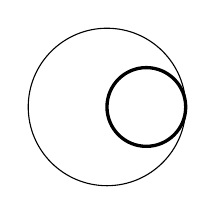
\begin{tikzpicture}[scale=.5]
\draw[very thick] (1,0) circle [radius=1];
\draw[scale=2] (0,0) circle [radius=1]; 
\end{tikzpicture}
\end{tikzshowenvi}
第二行的縮放 \texttt{scale} 是正常圖像的 \(0.5\times 2=1\) 倍。

使用負值來實現“翻轉”效果,以及使用 \tikzkw{scale around} 來指定縮放中心:
\begin{tikzshow}[very thick]
\draw[thin] (0,0) circle [radius=1];
\draw[xscale=-1] (0,0) rectangle (1,1);
\draw[red, xscale=-1] (0,0) rectangle (1,1);
\draw[blue, scale around={1.5:(1,1)}] (0,0) rectangle (1,1);
\end{tikzshow}

注意,縮放命令 \tikzkw{scale} 並不更改對象的屬性,比如點的字體大小、線寬等等。如果想要改變這些,參考\secref{subsec:nodescaling}部分。

\subsubsection{傾斜(slant)*}
傾斜不是一個常用的圖像變換。\tikzz\ 中的傾斜指令是 \tikzkw{xslant} 與 \tikzkw{yslant}。簡單地解釋,\texttt{xslant=k} 會把圖像中座標為 \((x,y)\) 的點變換為 \((x+k\times y, y)\)。
\begin{tikzshow}[very thick,scale=.6]
\draw[help lines] (0,0) grid (4,2);
\draw (0,0) -- (1,1) -- (1,2) -- cycle;
\draw[red, xslant=1.5] (0,0) -- (1,1) -- (1,2) -- cycle;
\draw[blue, xslant=-1] (0,0) -- (1,1) -- (1,2) -- cycle;
\end{tikzshow}

\subsection{裁剪(clip)}
在 \latexline{clip} 命令\RED{之後}的所有繪圖都會只顯示該裁剪視窗中的部分:
\begin{tikzshow}
\clip (0,0) rectangle (1.1, 1.1);
\draw[red, thick] (0,0) circle [radius=1];
\end{tikzshow}

添加 \tikzkw{draw} 選項可以把 \latexline{clip} 命令的“輪廓”繪製出來\footnote{也可使用 \latexline{draw} 命令並將 \tikzkw{clip} 作為參數,還可將兩者作為 \latexline{path} 命令的參數。}:
\begin{tikzshow}
\clip[preaction={draw=red,ultra thick}] (1.2,0) arc [start angle=0, end angle=225, radius=1.2];
\draw (-1,-1) rectangle (1,1);
\draw (-1,1) -- (1,-1);
\end{tikzshow}
上例使用一個非閉合的路徑(圓弧)來裁剪,\tikzz\ 會自動將其首尾連接。其中,\tikzkw{preaction} 選項表示在 \latexline{clip} 命令\RED{之前}先沿該路徑按傳遞給其的參數繪製,之後再創建裁剪視窗;這樣可以實現視窗輪廓的自定義繪製(因為裁剪隻影響其後的繪製命令)。

\subsection{分組(scope)}
\label{subsec:scope}
分組操作允許你對當前組使用參數——這些參數會疊加到全局參數上,並且不影響到組外的對象:
\begin{tikzshowenvi}
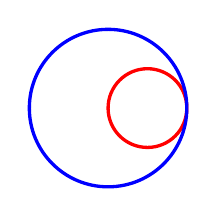
\begin{tikzpicture}[red, very thick, scale=.5]
\draw (1,0) circle [radius=1];
\begin{scope}[blue, scale=2]
\draw (0,0) circle [radius=1];
\end{scope}
\end{tikzpicture}
\end{tikzshowenvi}

\subsection{畫布大小}
命令 \latexline{useasboundingbox} 可以

\section{點(node)與文本}

\subsection{點的座標指定}
使用 \latexline{coordinate} 命令給點命名,便於之後引用。
\begin{tikzshow}
\coordinate (A) at (1,0);
\coordinate (B) at (1,1);
\draw (0,0) -- (A) circle[radius=.5] -- (B) -- cycle;
\end{tikzshow}
\tikzkw{coordinate} 也可以在繪製命令中作為選項使用。

\subsection{點的基本命令}
如需顯式地繪製點(即佔有面積的點),使用 \latexline{node} 命令,或者 \latexline{path} 命令的 \tikzkw{node} 選項,並配合 \tikzkw{draw} 選項。選項 \tikzkw{shape} 用於指定點的繪製方式。
\begin{tikzshow}
\node at (0,0) [shape=circle, draw] (C) {$p_C$};
\node at (1,0) [rectangle, draw, fill=red] {};
\path[yshift=1cm] (0,.5) node[draw] (A) {$p_A$}
     (1,.5) node[draw] (B) {$p_B$};
\draw (A) -- (B) -- (C);
\end{tikzshow}
選項 \tikzkw{shape} 還可賦值為 \texttt{coordinate},這樣在點之間連線時會從點中心開始繪製;但我建議此時直接使用 \tikzkw{coordinate} 命令。

\subsubsection{點的錨點(anchor)}
使用 \tikzkw{anchor} 選項定義錨點位置,可傳入的值是 4 個基本方位(east, west, south, north)、4 個複合方位(south west 等),以及 center。或者你可以依次用 left, right, above, below 來替代四個基本方位:
\begin{tikzshow}
\draw[help lines] (0,0) grid (2,2);
\draw (0,0) node [anchor=south west] {$\beta$};
\node at (0,1) [above right] {Here};
\node at (1,0) [above=2pt] {Hi};
\draw (1,2) node [below right=1pt and 8pt] {$1,0$};
\end{tikzshow}
其中,如果像最後一行給出雙距離參數,需加載 \pkg{positioning} 庫。

也可以直接用數字指定 \tikzkw{anchor} 的角度,\tikzz\ 會自動定位到點邊界上對應角度的位置:
\begin{tikzshow}
\draw (0,0) circle [radius=1];
\foreach \x in {1,...,12} {
  \node at (90-30*\x:1) [anchor=270-30*\x] {\x};
}
\end{tikzshow}

點的命名類似 \latexline{coordinate} 的用法:
\begin{tikzshow}
\path node (a) at (0,0) {}
      node (b) at (1,0) {};
\draw (a) -- (b);
\end{tikzshow}

\subsubsection{點的尺寸}
點的大小用 \tikzkw{inner sep} 指定文字到點邊框的距離,用 \tikzkw{minimum size} 指定邊框的最小尺寸。也可以配合 \tikzkw{text width} 選項指定文本的每行寬度。
\begin{tikzshow}
\tikzset{every node/.style={draw, circle}}
\node (a) {a};
\node[yshift=1cm] (b) {b};
\node[shift={(1,2)}, inner sep=2pt] (c) {c};
\node[xshift=1cm, minimum size=8pt] (d) {d};
\node[shift={(1,1)}, minimum size=8pt, inner sep=0pt] (e) {e};
\end{tikzshow}
注意點 \(d\) 和點 \(e\) 的區別。

\subsection{點的相對放置}
點的相對放置有兩種方式。其一如下例,雙距離語句需要 \pkg{positioning} 庫。
\begin{tikzshow}
\tikzset{every node/.style={draw, circle}}
\draw[help lines] (0,0) grid (3,3);
\node (a) {a};
\node (b) [above=of a] {b};
\node (c) [above right=.5cm and 2cm of b] {c};
\node (d) [below=.5cm of c, on grid] {d};
\draw[red] (b) rectangle (d);
\end{tikzshow}
\tikzkw{on grid} 選項表示從邊框而不是點中心開始計算距離,因此 \(b\) 與 \(d\) 的縱座標不同。另一種方式是使用方位詞結合點的名稱,組成 \texttt{點名\mbox{.}方位詞} 的語法:
\begin{tikzshow}
\node (a) {a};
\node[above] (aa) at (a.north) {a.north};
\end{tikzshow}
上例中的 \tikzkw{above} 選項不是必須的,但往往添加以避免點間的覆蓋。

\subsection{點的旁置文本(label/pin)}
旁置文本(或標籤)可用上一節的語法畫另一個點來實現,但 \tikzkw{label} 或 \tikzkw{pin} 選項更簡潔,會直接在主點旁畫一個旁置點。對同一個主點畫多個 \tikzkw{label} 或 \tikzkw{pin} 都是允許的;它們的區別在於後者會在主點和旁置點之間連一條線。

標籤位置的語法是 \texttt{角度\mbox{:}文本}——它還有一個特殊的角度參數 \texttt{center},會將標籤放在主點的中心處。你也可以通過 \tikzkw{label distance} 或 \tikzkw{pin distance} 選項來指定距離。
\begin{tikzshow}[every node/.style={draw, circle}]
\draw node[pin={[pin distance=.2cm, pin edge={<-, thick}]above right:$a_{p}$}] (a) at (0,0) {a} 
node[label={[red]30:$b'$}] (b) at (0,1) {b} 
node[label=120:$c'$, label=below:$c''$] (c) at (1.5,1) {c};
\end{tikzshow}
上例中甚至給 \tikzkw{label} 傳入了顏色參數。還可以使用 \texttt{every pin, every pin edge} 或 \texttt{every label} 樣式設定默認值。

當點被旋轉時,參數 \tikzkw{absolute} 可以幫助你定位。如果它的值是 \texttt{true} 或缺省,那麼方向不會跟隨點而旋轉,而是始終以紙面做參照:
\begin{tikzshow}
\tikzset{
    every node/.style={draw, rectangle},
    every label/.style={draw=red, font=\footnotesize}
}
\node[rotate=-80,label=right:label] (a) at (0,0) {normal};
\draw[blue, thick] (0,0) -- (-80:1);
\node[rotate=-80,label={[absolute]right:label}] (b) at (1,0) {absolute};
\draw[blue, thick] (1,0) -- +(0:1);
\end{tikzshow}
左側標籤的錨點(位於紅色矩形的左側邊上)在點“normal”右側邊框的中點,而右側標籤的錨點則位於穿過點“absolute”中心的水平向右的線上。\RED{上例中出現了方括號嵌套時,不要忘記添加花括號}。

\subsection{點的沿路徑文本}
\subsubsection{顯示指定}
將 \tikzkw{node} 選項放於對應的點座標之後,稱為顯示(explicitly)指定。

對於沿路徑的文本標記,\tikzz\ 預定義了 7 種位置,分別是 \tikzkw{at start/end}, \tikzkw{(very) near start/end},以及缺省時的 \tikzkw{midway}。
\begin{tikzshow}
\draw (0,0) .. controls (.5,2) .. (1.5,2)
  node[at start] {at start}
  node[midway, sloped, above] {midway}
  node[pos=1, right, text width=3ex] {at end};
\end{tikzshow}
上例中的一些參數:
\begin{para}
\item[sloped] 設置文字基線與圖中此處的切線平行。
\item[pos] 定量化的位置參數\footnote{並不是嚴格的空間分點;而是基於首、尾、控制點間向量計算出速度,取其時間分點。很難精確指定。}。比如預定義的 \tikzkw{very near start} 即為 \(0.125\),\tikzkw{near start} 即為 \(0.25\)。
\end{para}

對於交點指定(\tikzkw{|-} 或 \tikzkw{-|}),中點(\tikzkw{midway})即為垂足:
\begin{tikzshow}
\draw (0,0) |- (2,1) \foreach \p in {0,0.5,1} {
  node[pos=\p] {\p}
};
\end{tikzshow}

不同位置放置文本的場合,使用 \tikzkw{auto} 選項,並可以設定 \texttt{left} 或者 \texttt{right} 參數;選項 \tikzkw{swap} 則允許你將其文本放在對稱位置。注意:這兩個選項\RED{只對沿路徑的放置有效}。
\begin{tikzshow}[scale=.5, every node/.style={circle, inner sep=2pt}]
\foreach \x in {1,...,4} {
  \draw (90-90*\x:2) -- (-90*\x:2)
  node[midway, fill=red!30, auto=left] {\x}
  node[midway, fill=blue!30, auto, swap] {\x};
}
\end{tikzshow}

\subsubsection{隱式指定}
路徑裏點的位置可以隱式(implicitly)指定,放在 \texttt{--} 命令與要連接的點之間即可。只有隱式指定的點才會繼承全局參數(因此隱式指定往往可以省略一些參數,比如 \tikzkw{midway})。例子\cite{tikzmanual}:
\begin{tikzshowenvi}
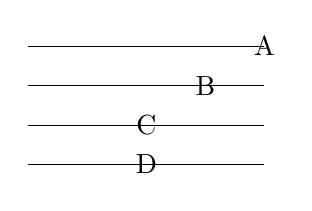
\begin{tikzpicture}[near end]
\draw (0,2.5) -- (3,2.5) node{A};
\draw (0,2) -- node{B} (3,2);
\draw (0,1.5) -- node[midway] {C} (3,1.5);
\draw (0,1) -- (3,1) node[midway] {D} ;
\end{tikzpicture}
\end{tikzshowenvi}
將上述代碼中的 \tikzkw{--} 換成 \tikzkw{to} 也可以;通常後者是個更強的命令,在下一節中也會介紹。

\subsection{點之間的連線}
\label{subsec:connectingnodes}
\subsubsection{基礎連線}
點之間連線會自動檢測點的繪製邊界,主要要三種操作方式:
\begin{enumerate}
\item 在點名稱後增加小數點和方位詞來指定,比如點 a 的左側就用 \texttt{(a.west)};
\item 使用 \texttt{to} 代替 \texttt{--},並附加 \tikzkw{out} 與 \tikzkw{in} 選項。(如果不附加則會畫直線)
\item 使用 \texttt{to} 附加 \tikzkw{bend left/right} 選項。下例中最後一行以 a 到 b 直線方向為角度 0,\texttt{bend left=45} 表示逆時針旋轉 $45$ 度作為 \tikzkw{out} 值,旋轉 $180-45=135$ 度作為 \tikzkw{in} 值。
\end{enumerate}
\begin{tikzshow}
\tikzset{every node/.style={draw,circle}}
\node (a) {a};
\node (b) [below=of a] {b};
\node (c) [left=of b] {c};
\draw[blue, ->] (c.north) .. controls +(up:1) and +(left:1) .. (a.west); 
\draw[red, ->] (c) [out=315, in=225] to (b);
\draw[->] (a) to [bend left=45] (b);
\end{tikzshow}

\subsubsection{繪製到命令(to)}
除了上面提到的 \tikzkw{to} 命令的用法,它還有以下靈活的使用方式:

使用 \tikzkw{edge node} 來給點之間的連接線添加文本。但更好用的是 \tikzkw{edge label} 命令,表示以 \tikzkw{auto} 選項來自動放置文本;如果換成 \tikzkw{edge label'},則表示以 \tikzkw{auto, swap} 選項放置。
\begin{tikzshow}
\coordinate (a);
\coordinate (b) at ($ (a)+(2,1) $);
\draw (a) to[edge node={node [sloped,above] {ab}}] (b);
\draw (a) to[color=red, bend right=45, edge label=auto, edge label'=swap] (b);
\end{tikzshow}

最後,該命令允許用户以 \tikzkw{to path} 選項來指定繪製方式,並用 \latexline{tikztostart} 表示當前 \tikzkw{to} 命令的起始點,\latexline{tikztotarget} 表示終止點,\latexline{tikztonodes} 表示繪製路徑時伴隨的點(可省略)。實質上是添加了一個路徑分組(花括號內的選項不會應用到外部):
\begin{latex}
{[every to, <options>] <path>}
\end{latex}

例子:
\begin{tikzshow}
\tikzset{selfloop/.style={to path={.. controls +(75:1) and +(105:1) .. (\tikztotarget) \tikztonodes}}}
\node (a) {$a$};
\node[right=of a] (b) {$b$};
\node[below=of b] (c) {$c$};
\draw[->] (a) edge (b) (b) edge[selfloop] node[above] {Hi} (b)  edge (c);
\end{tikzshow}
你可能注意到,上例中雖然定義了 \tikzkw{to path},但使用了 \tikzkw{edge} 而不是 \tikzkw{to};實質上兩者的語法有相近之處,但使用 \tikzkw{to} 會導致只有最後一條子路徑有箭頭。

庫 \pkg{topaths} 定義了一些實用的樣式,比如在上例中就可以直接使用它預定義 \tikzkw{loop above}。

\subsubsection{邊命令(edge)}
邊命令的底層形式是,其中 \verb|<path>| 與 \tikzkw{to} 格式相同:
\begin{latex}
\path[every edge, <options>] (\tikztostart) <path>
\end{latex}

因此它將繪製包含同一個點(即 \texttt{\char`\\tikztostart})的所有邊。當你想要給每個點的邊進行定製時,這會十分有用:
\begin{tikzshow}
\tikzset{every node/.style={draw,circle}}
\node (a) {a};
\node (b) [below=of a] {b};
\node (c) [left=of b] {c};
\draw[thick] (c) edge[red, -latex] (b)
    edge[bend left=45] (a)
    edge[blue, <-] (a);
\end{tikzshow}
提醒一下那些熟悉圖論的讀者:別忘了儘管最後一行中邊的箭頭方向是從 a 到 c 的,但仍可以像上面一樣用 c 點的 \tikzkw{edge} 命令來繪製。

你還可以連寫邊命令,並沿邊加上文字:
\begin{tikzshow}
\node foreach \name/\angle in {a/0,b/90,c/180,d/270}
    (\name) at (\angle:1.5) {$\name$};
\path[->] (b) edge node[above right] {$5$} (a)
  edge (c)
(c) edge [-,dashed, blue] node[auto] {auto}
  node[auto, swap] {swap} (a)
  edge (d)
(d) edge [red] node[above,sloped] {very}
  node[below,sloped] {red} (a);
\end{tikzshow}
這裏用到了之前提及的 \tikzkw{auto} 命令。注意,只要 \tikzkw{path} 命令指定了箭頭選項,\tikzkw{edge} 命令繪製的每條邊都有箭頭。

\subsection{點與畫布的縮放}
\label{subsec:nodescaling}


\subsection{作為圖像的點(pic)*}
一段繪圖代碼可能需要複用;如果它比較複雜,可以使用 \latexline{pic} 來重複調用。
\begin{tikzshow}[scale=0.8]
\tikzset{dcircle/.pic={\draw (0,0) circle [x radius=.5, y radius=.8] circle [radius=1];}}
% 兩種調用方式
\draw[help lines] (0,-1) grid (2,2);
\pic at (0,0) {dcircle}; 
\path (2,0) pic {dcircle};
\end{tikzshow}
語法非常類似 \tikzkw{node}。其中 \tikzkw{at} 也可以寫成 \texttt{[at=\{(0,0)\}]} 這種形式。

\tikzkw{pic actions} 選項用於傳入 \texttt{draw, fill, shade, 或 clip} 參數:
\begin{tikzshow}[scale=0.6, transform shape]
\tikzset{circlerect/.pic = {
    \path[pic actions] (.5,.5) circle [radius=.3];
    \draw (0,0) rectangle (1,1);
}}
\draw[red] (0,0) grid (4,2);
\pic [blue, thick] at (.5,.5) {circlerect};
\pic [draw=blue, fill=white] at (2.5,.5) {circlerect};
\end{tikzshow} 
當不傳入 \tikzkw{draw} 選項時,圓的 \latexline{path} 命令是不會繪製的;同時注意,因為繪製矩形的是 \latexline{draw} 命令,因此不受\tikzkw{fill} 選項影響。

插入的 \tikzkw{pic} 中的點可以在外部調用,一個例子:
\begin{tikzshow}
\tikzset{mypic/.pic={
  \draw[blue] (0,0) coordinate (-A)
  -- (1,1) coordinate (-B);
}}

\draw[help lines] (0,0) grid (1,2);
\pic (P) {mypic};
\pic (Q) at (0,1) {mypic};
\draw[red] (P-A) -- (Q-B);
\end{tikzshow}
\tikzkw{pic} 定義時用短橫命名是為了可讀性。調用時語法類似 \tikzkw{node}。

\pkg{quotes} 庫支持以加引號字串的方式傳入參數,作為 \tikzkw{pic text} 選項的值。比如 \texttt{angles} 這個預定義的 \tikzkw{pic}(由 \pkg{angle} 庫支持):
\begin{tikzshow}
\draw (0,-1) coordinate (P1)
  -- (0,0) coordinate (O)
  -- (1,1) coordinate(P2)
  pic [draw, "$\alpha$"] {angle=P1--O--P2};
\end{tikzshow}

一些其他注意:
\begin{feai}
\item 如果有 \texttt{foreach} 語句,\textbf{請放在 \texttt{pic} 定義的首行} 。
\item \tikzkw{pic} 雖説從用法上近似 \tikzkw{node},實質上它是以類似 \tikzz\ \envi{scope} 環境的方式工作的。因此,如果想要其外部的圖像變換對其生效,須添加 \tikzkw{transform shape} 選項於 \envi{tikzpicture} 環境。
\item \tikzkw{pic} 對象也能像 \tikzkw{node} 一樣,沿路徑放置,設置 \tikzkw{at start} 等選項。
\item 將 \tikzkw{pic} 作為選項使用時,添加 \tikzkw{behind path} 或者 \tikzkw{in front of path} 來指定將 \tikzkw{pic} 插入到所在路徑的下方或是上方圖層。
\item 如果你只是臨時使用而不想額外定義,這裏有一個使用 \tikzkw{code} 選項的例子\cite{tikzmanual}:
\begin{tikzshow}
\draw (0,0) .. controls(1,0) and (2,1) .. (3,1)
foreach \t in {0, 0.1, ..., 1} {
  pic [pos=\t] {
    code={\draw circle [radius=2pt];}
  }
};
\end{tikzshow}
注意,本例只有一句語句。句中 \tikzkw{pic} 是 \latexline{draw} 命令的選項。
\end{feai}

\section{路徑(path)}
雖然我們不常直接使用 \latexline{path} 命令,而是使用它的變體 \latexline{draw} 等,但是我們仍然需要介紹一些它的特性。

最常用的情景就是隻聲明點,但卻不顯示地繪製它們:
\begin{tikzshow}
\path coordinate (a)
     coordinate[right=of a] (b)
     coordinate[above=of b] (c);
\draw (a) -- (b) -- (c) -- cycle;
\end{tikzshow}

特別指明,點命令(\tikzkw{node} 或者 \tikzkw{coordinate})總是在路徑繪製結束後再繪製的;它們不是路徑的一部分。

以下路徑命令已在上文(或將在其他小節)進行介紹:
\begin{description}
\item[移動(move-to)指令] 隱式。如 \verb|draw (a) -- (b) (c) -- (d)|,在 b 與 c 間即為移動指令。
\item[直線(line-to)指令] 包括直線指令 \tikzkw{--} 與水平豎直線指令 \tikzkw{|-} 和 \tikzkw{-|}。
\item[曲線(curve-to)指令] 即繪製 \bz\ 曲線的 \tikzkw{.. controls ..} 指令。
\item[繪製到(to)指令] 上文介紹過 \tikzkw{to} 配合 \tikzkw{out, in, bent left} 等命令的用法,參考前文\secref{subsec:connectingnodes}。它實際將指令解釋為以上三種指令之一。
\item[幾何形狀指令] 包括圓或橢圓 \tikzkw{circle}、矩形 \tikzkw{rectangle} 與弧 \tikzkw{arc} 指令。
\item[函數指令*] 包括拋物線 \tikzkw{parabola}、正弦 \tikzkw{sin} 與餘弦 \tikzkw{cos} 指令。更復雜的函數會在
\item[網格指令] 即 \tikzkw{grid} 指令。
\item[圓角指令*] 即 \tikzkw{rounded corners} 與 \tikzkw{sharp corners} 指令。
\item[循環指令] 即 \tikzkw{foreach} 指令,具體可參考\secref{subsec:foreach}部分。
\item[暫存指令] 即 \tikzkw{let} 指令,將數據暫存以供語句之後調用。參考\secref{subsec:nodesdistance}部分。
\item[圖指令*] 即 \tikzkw{graph} 指令,繪製圖、樹、網絡的命令。參考\secref{sec:network}部分。
\item[圖像指令*] 即 \tikzkw{pic} 命令,
\end{description}

本節會介紹除上述指令外的其他路徑指令。

\subsection{路徑分組}
類似與 \envi{scope} 環境,\tikzz\ 允許在路徑中創建一個“分組”,分組中的選項不會影響到分組外部的內容。只需要將想要建立分組的部分用花括號包圍即可:
\begin{tikzshow}
\path coordinate (a)
     coordinate[right=of a] (b)
     coordinate[above=of b] (c)
     coordinate[left=of c] (d);
\draw (a) -- (b) {[rounded corners] -- (c) -- (d) {[sharp corners] -- cycle}};
\end{tikzshow}
注意,並不是所有參數都支持分組。例如,每條路徑只能有一個顏色,因此在分組中指定另一種顏色是無效的。

\subsection{SVG 指令*}
加載 \pkg{svg.path} 庫後,路徑中的 \tikzkw{SVG} 選項允許你使用類似網頁 \texttt{HTML} 中 \texttt{SVG} 的語法進行繪製。這裏不再詳細對 SVG 語法做説明,僅給出一個例子:
\begin{tikzshow}
\draw[fill=red!50] svg {M 0 0 L 10 10 h 20 v -10} -- cycle;
\end{tikzshow}
該庫只支持真正的 \texttt{SVG} 指令集的主要部分,並不是完全涵蓋。

\subsection{繪圖指令(plot)}
該指令用於繪製點較多的圖,也可以從外部文件讀取。

\subsection{計算指令(pgfextra)}
該指令只能用於路徑命令內部,運行到此處時路徑繪製會掛起,直到運行完該命令內部的部分再繼續繪製。一個例子:
\begin{tikzshow}
\newdimen\myloc
\myloc=0cm
\draw (0,\myloc) \pgfextra{\myloc=.5cm}
    circle [radius=\myloc] -- (0,1);
\end{tikzshow}

\section{數學繪製:幾何與函數圖像}
嚴格的幾何學繪圖需要一些特別的命令,比如計算兩點間的距離。而且,通常會使用 \tikzkw{coordinate} 而不是 \tikzkw{node} 命令;因為前者並不佔用面積,這樣畫線時才能保證抵達點所在的中心座標。

\subsection{座標計算}
庫 \pkg{calc} 允許用户使用 \texttt{\$ ... \$} 的形式來計算,並放在一對圓括號中作為座標:
\begin{tikzshow}
\coordinate[label=below:A] (A);
\coordinate[above right=.5 and 1.5 of A, label=right:B] (B);
\draw (A) -- (B);
\draw ($ (A) + (.3,.4) $) circle (.5);
\end{tikzshow}

\subsection{兩點距離計算}
\label{subsec:nodesdistance}
上一節中的半徑值是人工計算的。下例讓 \tikzz\ 計算距離,並用 \tikzkw{let} 選項將其儲存起來,在 \tikzkw{in} 選項的後方進行調用:
\begin{tikzshow}[scale=0.6, transform shape]
\coordinate[label=left:A] (A);
\coordinate[above right=.5 and 1.5 of A, label=right:B] (B);
\draw (A) -- (B);
\draw let \p1 = ($ (B) - (A) $),
         \n{rad} = {veclen(\x1,\y1)}
      in (B) circle[radius=\n{rad}]
         (A) circle[radius=\n{rad}];
\end{tikzshow}
命令 \verb|\p<數字>| 用於存儲向量計算結果,比如 \verb|\p1|。對應的,使用 \verb|\x1| 或者 \verb|\y1| 可以調用向量的兩個座標值。而 \verb|\n<數字>| 則用於存儲數值。此外,命令 \tikzkw{veclen} 用於計算向量的歐式長度 \(\sqrt{x^2+y^2}\)。  

如果不想使用數字命名,可以像上例的存儲數值一樣使用字符串;不過這樣命名需要加上花括號。事實上,已知圓心 $A$ 和圓周上一點 $B$,有更簡單的畫圓方法,參考\secref{subsec:circlethrough}部分的內容。

\subsection{$\lambda$分點與垂線}
\subsubsection{比例分點}
分點是幾何中常用的概念,\pkg{calc} 庫支持像 \pkg{xcolor} 混合顏色類似的命令:\verb|<點A>!<分點比例>![角度]<點B>|,不同的是“角度”會將分點位置繞 A 旋轉一個角度。將它還可以用最後一行中鏈式的方法進行連寫:
\begin{tikzshow}
\coordinate[label=left:A] (A);
\coordinate[above right=.5 and 1.5 of A, label=right:B] (B);
\coordinate (X) at ($ (A)!0.5!(B) $);
\coordinate[label=above:C] (C) at ($ (X)!{sqrt(3)}!90:(B) $);
\path[draw=black, fill=blue!20] (A) -- (B) -- (C) -- cycle;
\node[draw=black, fill=red!20, circle through=(X)] at ($ (A)!0.5!(B)!{tan(30)}!90:(B) $) {};
\end{tikzshow}

\subsubsection{距離分點}
你也可以用(直線段)分點距離代替分點比例,加上單位即可:
\begin{tikzshow}
\coordinate[label=left:A] (A);
\coordinate[above right=.5 and 1.5 of A, label=right:B] (B);
\coordinate (C) at ($ (A)!0.5!(B) $);
\draw ($ (C)!1cm!90:(B) $) edge (B) edge (A)
     edge[dashed] node[above, sloped, font=\footnotesize] {1cm} (C);
\end{tikzshow}

\subsubsection{投影分點(垂線)}
用投影點代替分點比例,則得到該點向連線段的投影:
\begin{tikzshow}
\coordinate[label=left:A] (A);
\coordinate[above right=.5 and 2 of A, label=right:B] (B);
\coordinate[above right=1 and .5 of A, label=above:C] (C);
\draw (A) -- (B) -- (C) -- cycle;
\draw[red] (C) -- ($ (A)!(C)!(B) $);
\end{tikzshow}

\subsection{過某點的圓*}
\label{subsec:circlethrough}
使用 \pkg{through} 庫可以方便地畫出給定圓心和過某點的圓,而不需要做兩點距離計算:
\begin{tikzshow}[scale=0.6]
\coordinate[label=below left:A] (A);
\coordinate[above=1 of A, label=above right:B] (B);
\draw (A) -- (B);
\node[draw, circle through=(B), label=left:C] at (A) {};
\node[draw, circle through=(A), label=right:D] at (B) {};
\end{tikzshow}
注意,\tikzkw{circle through} 僅僅適用於 \tikzkw{node} 命令。

\subsection{交點}
在\secref{subsec:intersection}中已經介紹過交點的使用,包括 \tikzkw{-|} 指令與 \pkg{intersections} 庫的一些用法。這裏的例子更復雜一些,也複習了之前等分點的用法:
\begin{tikzshow}
\tikzset{small/.style={draw, circle, fill=black, inner sep=1pt}}
\coordinate[label=left:A] (A);
\coordinate[above right=.5 and 1.5 of A, label=right:B] (B);
\coordinate[label=below:C] (C) at ($ (A)!0.5!(B) $);
\coordinate (D) at ($ (C)!2!90:(B) $);
\coordinate (E) at ($ (C)!2!-90:(B) $);
\draw (A) -- (B);
\draw[red, name path=Lv] (E) -- (D);
\node[draw, circle through=(B), name path=Ca] at (A) {};
\path[name intersections={of=Lv and Ca, by={[label=above right:D]D, [label=right:E]E}}];
\foreach \x in {A,C,D,E}
  \node[small] at (\x) {};
\end{tikzshow}
注意上例中的 \latexline{path} 命令雖聲明瞭交點,但沒有畫任何內容。

\section{圖與網絡繪製*}
\label{sec:network}

\section{屬性}
\label{sec:tikz-property}

\subsection{線寬}
\tikzz\ 預定義了 7 種線寬,從細到粗是:\tikzkw{ultra thin}, \tikzkw{very thin}, \tikzkw{thin}, \tikzkw{semithick}, \tikzkw{thick}, \tikzkw{very thick}, \tikzkw{ultra thick}。或者利用 \tikzkw{line width} 選項指定。
\begin{tikzshow}
\draw[ultra thin] (0,0) -- (1,0);
\draw[ultra thick] (1,0) -- (2,0);
\draw[line width=10pt] (0,1) -- (2,1);
\end{tikzshow}
初始線寬是 0.4pt;兩個 \tikzkw{ultra} 線寬分別是 0.1pt 與 1.6pt。

\subsection{線型}
\tikzz\ 預定義了 4 種基本線型:\tikzkw{dashed}, \tikzkw{dotted}, \tikzkw{dash dot}, \tikzkw{dash dot dot}。它們還可以配合 \tikzkw{loosely} 或者 \tikzkw{densely} 進行微調。
\begin{tikzshow}
\draw[dashed] (0,0) -- (1,0);
\draw[dotted] (0,-0.5) -- (1,-0.5);
\draw[dash dot] (0,-1) -- (1,-1);
\draw[dash dot dot] (0,-1.5) -- (1,-1.5);
\draw[loosely dashed] (0,-2) -- (1,-2);
\draw[densely dotted] (0,-2.5) -- (1,-2.5);
\end{tikzshow}

如果的確需要深度自定義,請使用 \tikzkw{dash pattern} 自定義線型,並可配合 \tikzkw{dash phase} 指定線型的起始位置。
\begin{tikzshow}
\draw[dash pattern=on .1cm off .25cm on .25cm off .15cm, dash phase=1cm] (0,0) -- (3,0);
\end{tikzshow}

有時你可能會看到一些複雜的裝飾線(需要 \pkg{decorations} 庫),比如:\tikz{\draw [->,decorate,decoration=snake] (0,0) -- (2,0)}。請參考\secref{subsec:deco}。

\subsection{線尾(line cap)*}
如果線寬度較大,不同的線尾 \tikzkw{line cap} 明顯對應不同的效果:
\begin{tikzshow}[every label/.style={font=\footnotesize}]
\foreach \offset/\s in {0/rect, .5cm/butt, 1cm/round} {
    \draw[yshift=\offset,line width=5pt, line cap=\s] (0,0) -- (1,0)  node[label=right:\s] {};
    \draw[yshift=\offset, white] (0,0) -- (1,0);
}
\end{tikzshow}

\subsection{線交(line joint)*}
連續畫線時(非連續畫線處此選項無效),可以設置 \tikzkw{line joint}:
\begin{tikzshow}[every label/.style={font=\footnotesize}]
\foreach \offset/\s in {0/round, 1.25cm/bevel, 2.5cm/miter} {
    \draw[xshift=\offset,line width=5pt, line join=\s] (0,0) -- (.5,1) node[label=above:\s] {} -- (1,0)  ;
}
\end{tikzshow}
其中 \tikzkw{miter} 線交在鋭角時會產生一個非常“尖”的效果,可以設置 \tikzkw{miter limit} 參數來設置一個角度值,使小於該角度的 \tikzkw{miter} 線交自動轉變為 \tikzkw{bevel} 形式。

\subsection{箭頭}
\tikzz\ 中的箭頭使用的細節多到可以單獨開一個章節,但我並不想全部詳盡地介紹。用大於或小於號表示箭頭的指向,用豎線表示是否加上截斷符號。一些基本的樣例:
\begin{tikzshow}
\draw[->|] (1,3) -- (2,3);
\draw[stealth-] (1,2) -- (2,2);
\draw[->,>=stealth, line width=3pt] (1,1) arc [start angle=90, end angle=30, radius=1];
\draw[<->] (.5,4) -- (.5,0) -- (2.5,0);
\end{tikzshow}
其中,用 \texttt{>=stealth} 或 \texttt{-stealth} 的方式指定了箭頭末端的類型為 \texttt{stealth}。你也可以將它們作為整個 \envi{tikzpicture} 環境的參數進行傳遞。

\tikzz\ 的 \pkg{arrows.meta} 庫包含很多箭頭,讀者可以自行查閲。

\subsection{繪製顏色}
在繪製網格一節,已經使用過 \texttt{lightgray} 作為網格的繪製顏色;當時省略了 \tikzkw{color} 選項。該選項設定\RED{除了 shading 外的所有}顏色,包括繪製、填充等:
\begin{tikzshow}
\path[draw,fill,red!50] (0,0) -- (1,0) circle[radius=.5];
\end{tikzshow}
注意:單獨使用 \latexline{draw} 或者 \latexline{fill} 只會執行繪製或填充其一,除非詳細指定局部的參數。

可以使用 \tikzkw{draw} 來單獨指定繪製的顏色:
\begin{tikzshow}
\draw[draw=red!50!white, ultra thick] (0,0) rectangle (1,1);
\end{tikzshow}
其中,雙感嘆號加數字是表示插值比例為 0.5;\pkg{xcolor} 宏包支持該語法。常用的顏色包括:
\begin{tikzshow}
\tikzset{every pin/.style={pin distance=.5cm, font=\footnotesize, inner sep=0pt}}
\draw (0,0) circle[radius=1];
\foreach \c[count=\i] in {red,green,blue,cyan,magenta,yellow,black,
lightgray,gray,darkgray,white,brown,
lime,olive,orange,pink,purple,teal,violet}
\node[circle,draw=black, fill=\c, pin={[pin edge={draw=\c, thick}] 90-360/19*\i:\c}] at (90-360/19*\i:1cm) {};
\end{tikzshow}

在 \tikzz\ 環境內部,還可以使用 \latexline{colorlet} 或者 \latexline{definecolor} 自定義顏色(它們實際上是 \TeX\ 指令),例如:
\begin{latex}
\colorlet{linecolor}{red!60!black}
\definecolor{fillcolor}{rgb}{1,0.5,1}
\end{latex}

\subsection{單色填充}
填充命令 \latexline{fill} 只能使用於閉合區域,\textbf{且不繪製區域邊界}。你可以在一般繪製命令的末尾添加 \tikzkw{cycle} 來創建一個閉合對象:
\begin{tikzshow}
\fill[green] (0,0) -- (1,0) -- (1,1) -- cycle;
\end{tikzshow}

在填充的同時繪製\footnote{準確地説,\latexline{filldraw} 命令是先繪製再填充。},使用 \latexline{filldraw} 命令,並分別指定繪製和填充顏色:
\begin{tikzshow}
\filldraw[draw=black, fill=cyan] (0,0) -- (2,0) arc (0:30:2);
\end{tikzshow}
\tikzkw{filldraw} 填充的區域會比用 \tikzkw{fill} 稍大一些,因為前者考慮了線寬。

要了解填充的細節,需要介紹兩個區域特性:
\subsubsection{非零區域}
該特性是默認的區域特性。\tikzz\ 使用計數器的方式來區分路徑的內部與外部。對於某點的判斷,它會從該點發射一條到無窮遠的射線;如果沿途的路徑是從左到右(順時針)地與這條射線相交,那麼計數器加一;反之減一。最後計數器如果是零,那麼該點在路徑外部;否則,它在區域內部。

下例逆時針地繪製了小矩形、順時針地繪製了完全圍住小矩形的大矩形。這樣小矩形的內部被識別為“外部”,因此未被填充。
\begin{tikzshow}
\filldraw[fill=blue!50] (0,0) -- (0,.5) -- (1,.5) -- (1,0) -- cycle
  (-.5,-.5) -- (1.5,-.5) -- (1.5,1) -- (-.5,1) -- cycle;
\end{tikzshow}

\subsubsection{奇偶區域}
奇偶區域也會發射一條射線,但只要遇到路徑就會計數器加一。利用區域的奇偶性填充,使用 \tikzkw{even odd rule}:
\begin{tikzshow}
\fill[even odd rule, blue] (0,0) -- (2,0.5) -- (1,1) circle (0.25);
\end{tikzshow}

\subsection{圖案與圖像填充*}
在指定了 \tikzkw{pattern} 選項時,它會自動進行填充操作(即使你使用的是 \latexline{draw} 命令)。要使用圖案填充,請加載 \pkg{patterns} 庫。
\begin{tikzshow}
\draw[pattern=dots, pattern color=red] (0,0) rectangle (1,1);
\end{tikzshow}

圖像填充允許你使用外部圖像,或者一般的 \tikzz\ 命令。注意配合 \tikzkw{path picture bounding box} 使用。
\begin{tikzshow}

\end{tikzshow}

\subsection{漸變填充*}
使用 \latexline{shade} 命令控制漸變填充,

\subsection{透明度*}
p169

\subsection{雙線*}
雙線選項在某些場合也是實用的。可以用 \tikzkw{double distance} 指定雙線內間距(默認 0.6pt),或者用 \tikzkw{double distance between line centers} 指定雙線的中心間距。
\begin{tikzshow}
\draw[double] (0,0) -- (1,1);
\draw[draw=white, double=cyan] (1,0) -- (0,1);
\draw[double distance=1pt] (1.2,0) -- (1.2,.5);
\draw[double distance=1pt,thick] (1.2,.5) -- (1.2,1);
\end{tikzshow}
上例的 \tikzkw{draw} 指定為白色,實質創造一種“從上方穿過”的效果。

還有一個特殊的雙線選項 \tikzkw{double equal sign distance},可以將雙線間距設置成與當前字體的等號($=$)間距一致。

\section{樣式與高級控制}
\subsection{樣式(style)}
如果某種屬性需要用來反覆作圖,可以把它自定義為樣式:

上文中出現過的 \texttt{help lines},就是 \tikzz\ 預定義的一種樣式。其相當於於:
\begin{latex}
\begin{tikzpicture}[help lines/.style={line width=0.2pt,gray}]
...
\end{tikzpicture}
\end{latex}

你也可以在進入 \tikzz\ 環境後(或在文檔導言區),使用 \latexline{tikzset} 命令來定義。

\subsection{循環語句(foreach)}
\label{subsec:foreach}
\tikzz\ 支持循環語句,這一點對於科技繪圖來説十分重要。
\begin{tikzshow}[place/.style={circle, draw, fill=black, minimum size=5pt, inner sep=0pt}]
\foreach \x in {1,2,3} {
    \node at (\x, 0) [place] {};
    \draw (\x, 0) circle [radius=1/\x];
}
\end{tikzshow}

有時候我們需要循環一個等差數列,這時候使用 \ldots\ 即可。\tikzz\ 會將 \(a,b,\ldots,c\) 識別為從 \(a\) 到 \(c\) 以 \(b-a\) 為公差的等差數列;如果你不指定 \(b\),那麼默認以 \(1\) 為公差。
\begin{tikzshow}[place/.style={circle, draw, fill=black, minimum size=5pt, inner sep=0pt}]
\foreach \x in {1,1.5,...,3,4} {
    \node at (\x, 0) [place] {};
    \draw (\x, 0) circle [radius=\x/8];
}
\end{tikzshow}
上例中的 \(4\) 不在數列內,這樣寫是允許的。數列後也可以接另一個數列。

大部分需要知道“循環到列表第幾個”的場合,都可以配合移動畫筆或相對座標命令實現:
\begin{tikzshow}[scale=.5]
\draw[red] (0,0) grid (3,3);
\foreach \x/\y in {0,1/2,2}
  \draw (\x, \y) +(.5,.5) circle [radius=.4];
\end{tikzshow}
上例同時循環了多個變量,中間用斜線分隔;它們分別按照列表中斜線分隔後的對應值進行循環。如果某一位置的列表提供值的個數小於變量的個數,那麼“多出”的變量將都取最後一個值。

此外,如果 \latexline{foreach} 內部只有一條語句,像上例一樣不加花括號也可以。

\subsection{圖層*}
一般情況不會用到此指令。但有時你需要先畫完上層的內容才能確定下層元素的尺寸,這時候可能需要圖層\cite{tikzmanual}(需要 \pkg{backgrounds} 庫):
\begin{tikzshow}
\tikzset{every node/.style={draw,circle,inner sep=.1cm, minimum size=.8cm}}
\foreach \x/\pos in {{a/(0,0)},{b/(1.5,0)},{c/(1,-1)}}
    \node (\x) at \pos {\x};
\draw (b.east) .. controls +(0:1) and +(0:1) .. (c.east);
\begin{scope}[on background layer]
    \node[draw=none,fill=lightgray, rectangle, fit=(b) (c)] {};
\end{scope}
\end{tikzshow}
上例中還使用了 \pkg{fit} 庫,用來創建一個“遮蓋”點 b 和點 c 的背景點——這個點的矩形邊框被 \tikzkw{fit} 命令處理成圖中的大小。

\subsection{裝飾*(decorations)}
\label{subsec:deco}
最簡單的裝飾是蛇形線\cite{tikzmanual},需要 \pkg{decorations.pathmorphing} 庫:
\begin{tikzshow}
\draw[->,decorate,decoration=snake] (0,0) -- (2,0);
\end{tikzshow}

通常,我們希望在線段結束就終止裝飾(否則會蛇形繪製到線段末尾,這可能引起困惑)。下面是一個複雜的例子:
\begin{tikzshow}
\draw[->, decorate, decoration={snake,amplitude=.4mm,segment length=4mm,post length=2mm}] (0,0) -- (3,0)
    node[above, align=center, midway, text width=2.5cm, font=\footnotesize] {
        multiline text controlled by \texttt{text width} option of \textcolor{blue}{node}
    };
\end{tikzshow}
大部分的參數都比較好理解。\tikzkw{amplitude} 控制波動的強弱,\tikzkw{segment length} 控制一個週期的長度,\tikzkw{post length} 控制在終點之前何處結束裝飾。

\subsection{隨機數*}
\tikzz\ 使用 \tikzkw{rand} 來生成從 $-1$ 到 $1$ 的隨機數(服從均勻分佈);如果使用 \pkg{calc},你還可以在指定座標時使用 \texttt{(\$...\$)} 並在其中做座標計算: 
\begin{tikzshow}
\makeatletter\def\pgfcurrentseed{
  \pgfmathparse{\pgfmath@rnd@z}\pgfmathresult
}\makeatother
\coordinate [label=left:$A$] (A) at (.5*rand,.5*rand);
\draw (0,0) node[below=1] {\pgfcurrentseed} circle [radius=1];
\coordinate [label=left:$B$] (B) at ($ (0,0) + (rand,rand)$);
\path (0,0) node[above=1] {\pgfcurrentseed};
\end{tikzshow}
上例中在 \TeX\ 底層中使用 pgf 命令從 \latexline{pgfmath@rnd@z} 中讀取當前隨機數種子的值,並賦給自定義命令。每次使用 \tikzkw{rand} 命令都會改變隨機數種子的值。

\subsection{外部數據文件*}

\section{實用範例}
\label{sec:tikz-eg}
本節通過例子的方式,向讀者展示 \tikzz\ 的常用情形。

% Appendices

% 參考文獻
\bibliography{Bib}

% 附錄
\clearpage
\appendix
% 重定義附錄的chapter樣式
\renewcommand{\chaformat}[1]{%
	\parbox[b]{.5\textwidth}{\raggedleft\bfseries \S 附錄 \\ \vspace{0.2ex} #1} \quad\rule[-12pt]{2pt}{70pt}\quad
	{\fontsize{60}{60}\selectfont\thechapter}}

\chapter{注音符號}
\label{app:phonetic}
% 這裏不用>{\ttfamily}而用\verb是為了減少報錯可能
\begin{center}
\tabcaption{注音符號與特殊符號}
\begin{tabular}{|*{4}{>{\centering}p{3em} @{-\hspace{1em}} p{3em}|}}
\hline
\texttt{樣式} & 命令 & \texttt{樣式} & 命令 & \texttt{樣式} & 命令 & \texttt{樣式} & 命令 \\
\hline
\=o  & \verb|\=o|  & \'o  & \verb|\'o|  & \v o & \verb|\v o|  & \`o   & \verb|\`o|  \\
\^o  & \verb|\^o|  & \"o  & \verb|\"o|  & \.o  & \verb|\.o|   & \H o  & \verb|\H{o}| \\
\d o & \verb|\d{o}| & \u o & \verb|\u{o}| & \b o & \verb|\b{o}|  & \t oo & \verb|\t{oo}|\\
\multicolumn{2}{|c@{\bf --}}{$\tilde{o}$} & \multicolumn{2}{@{\bf --}c|}{\tt{\$$\backslash$tilde\{o\}\$}} &%
\multicolumn{2}{c@{\bf --}}{$\hat{o}$}    & \multicolumn{2}{@{\bf --}c|}{\tt{\$$\backslash$hat\{o\}\$}}\\
\multicolumn{8}{|c|}{} \\
\o  & \verb|\o|  & \O  & \verb|\O|  & \i  & \verb|\i|  & \j  & \verb|\j| \\
\aa & \verb|\aa| & \AA & \verb|\AA| & \ae & \verb|\ae| & \AE & \verb|\AE|\\
\oe & \verb|\oe| & \OE & \verb|\OE| & !`  & \verb|!`|  & ?`  & \verb|?`| \\
\hline
\end{tabular}
\end{center}

\mbox{}

\begin{center}
\tabcaption{國際音標輸入表(部分)}
\begin{tabular}{|*{3}{>{\rmfamily}c !{-} >{\ttfamily}p{7.5em}|}}
\hline
\texttt{樣式} & 命令 & \texttt{樣式} & 命令 & \texttt{樣式} & 命令 \\
\hline
\textdzlig & \char92textdzlig & \textesh & \char92textesh & \textteshlig & \char92textteshlig \\
\textdyoghlig & \char92textdyoghlig & \textturnv & \char92textturnv & \textschwa & \char92textschwa \\
\textscriptg & \char92textscriptg & \texttheta & \char92texttheta & \textupsilon & \char92textupsilon \\
\textscripta & \char92textscripta & \dh & \char92dh & \textepsilon & \char92textepsilon \\
\textopeno & \char92textopeno & \textyogh & \char92textyogh & \ng & \char92ng \\
\hline
\multicolumn{2}{|c|}{重音} & \multicolumn{2}{c|}{次重音} & \multicolumn{2}{c|}{長音節} \\
\textprimstress & \char92{}textprimstress & \textsecstress & \char92textsecstress & \textlengthmark & \char92textlengthmark \\
\hline
\end{tabular}
\end{center}

\textit{注:\texttt{\char92dh}命令在非CJK文檔中有時編譯會出現問題}.

\chapter{建議與其他}

除了參考文獻列表中給出的書籍以外,我還推薦你用控制枱在\TeX{} Live中能找到的以下書籍:

\medskip\begin{para}
\item[texdoc usrguide] \TeX\ Live自帶的用户手冊.
\item[texdoc clsguide] \TeX\ Live自帶的文檔類和宏包編寫手冊.
\item[texdoc fntguide] \TeX\ Live自帶的字體使用手冊.
\item[texdoc symbols-a4] 一份速查表,基本上所有的\LaTeX\ 字符命令都在這裏了.
\item[texdoc latexcheat] 很有趣的命令表,只有兩頁.
\item[texdoc impatient] \emph{\TeX{} for the Impatient}, 一本介紹底層\TeX\ 的書.這也是我閲讀的第一本\TeX\ 書,Knuth的\emph{The \TeX\ book}雖然血統正但是難啃啊.本書中譯本在:\url{https://bitbucket.org/zohooo/impatient/wiki/Home}
\item[texdoc texbytopic] \emph{\TeX{} by Topic}, 個人覺得不如上面那本,但也許只是敍述方式不一樣吧.
\end{para}
\bigskip

\noindent 你可能還需要的功能:
\begin{description}
\item[\pkg{mhchem}] 該宏包用於輸入化學式,提供了\latexline{ce}命令.
\end{description}

% \tikzz\ 索引
%\setlength{\columnseprule}{0pt}
%\printindex

\end{document}
